\documentclass[11pt,a4paper]{amsart}

\usepackage{amsmath,amssymb,amsthm,mathtools}
\usepackage[T1]{fontenc}
\usepackage[utf8]{inputenc}
\usepackage{lmodern}
\usepackage{microtype}
\usepackage{hyperref}
\usepackage{orcidlink}
\usepackage{enumitem}
\usepackage{booktabs}
\usepackage{graphicx}
\usepackage[table]{xcolor}
\usepackage{pgfplots}
\usepgfplotslibrary{groupplots}
\pgfplotsset{compat=1.18}
\usepackage[margin=1in]{geometry}
\raggedbottom

\theoremstyle{plain}
\newtheorem{theorem}{Theorem}[section]
\newtheorem{proposition}[theorem]{Proposition}
\newtheorem{lemma}[theorem]{Lemma}
\newtheorem{corollary}[theorem]{Corollary}

\theoremstyle{definition}
\newtheorem{definition}[theorem]{Definition}
\newtheorem{assumption}[theorem]{Assumption}

\theoremstyle{remark}
\newtheorem{remark}[theorem]{Remark}

\DeclareMathOperator{\Var}{Var}
\DeclareMathOperator{\Cov}{Cov}
\DeclareMathOperator{\tr}{tr}
\DeclareMathOperator{\rank}{rank}
\DeclareMathOperator{\spanop}{span}
\DeclareMathOperator{\diag}{diag}
\newcommand{\R}{\mathbb{R}}
\newcommand{\N}{\mathbb{N}}
\newcommand{\PP}{\mathbb{P}}
\newcommand{\QQ}{\mathbb{Q}}
\newcommand{\EE}{\mathbb{E}}
\newcommand{\one}{\mathbf{1}}
\newcommand{\dd}{\,d}
\newcommand{\toP}{\xrightarrow{\PP}}
\newcommand{\toD}{\xrightarrow{d}}
\newcommand{\scrT}{\mathcal{T}}
\newcommand{\scrB}{\mathcal{B}}
\newcommand{\scrI}{\mathcal{I}}
\newcommand{\scrY}{\mathcal{Y}}

\begin{document}

\title[Detecting Latent Volatility Contagion]{%
Detecting Latent Volatility Contagion\\[0.3em]
{\small A Projected Score Estimator for Rough Volatility Models}}
\author[J.~Vidal Llaurad\'o]{J.~Vidal Llaurad\'o\,\orcidlink{0009-0002-1918-5458}}
\thanks{DOI: \href{https://doi.org/10.2139/ssrn.6616118}{10.2139/ssrn.6616118}.}
\email{vidal.llaurado@gmail.com}
\subjclass[2020]{60G22, 62M15, 62F12, 91G80}
\keywords{rough volatility, latent volatility contagion, projected covariance scores, source-screened inference, Gaussian Volterra models, high-frequency realized volatility, Oxford-Man realized library}
\date{April 2026}

\begin{abstract}
Roughness can be estimated from option surfaces or from realized-volatility paths, but directed
volatility contagion is a different object.  It is the source-screened component of the
source-target covariance derivative after the target-only tangent space has been removed.  This
paper turns that component into a projected covariance-score estimator and applies it to a balanced
Oxford-Man realized-volatility panel of eight global equity indices.  Pricing visibility,
path-space detectability, and observable-history screening remain distinct restrictions on the same
local estimand.

The econometric experiment is a reduced local Gaussian block model.  Local alternatives enter
through covariance derivatives; target-only covariance scores are projected out; the remaining
source-incremental derivative is estimated by a low-dimensional projected covariance-score GMM
statistic.  The score geometry yields local Gaussian efficiency constants, a rough-regime projected
rank condition, pilot-adaptive transfer under logarithmic roughness accuracy, and a uniform minimax
statement once the primitive Volterra reduction and projected-rank inputs hold uniformly.  Synthetic
experiments check the implementation against closed-form information and noncentrality constants.

On the Oxford-Man panel the estimated physical-measure roughnesses lie between about 0.04 and
0.09.  For SPX the estimator gives \(H_{\PP}\approx0.071\), while the external projected
option-surface benchmark of Livieri, Mouti, Pallavicini, and Rosenbaum (2018) gives
\(H_{\mathrm{imp}}\approx0.30\).  The full-sample \(\PP\)-side directed contagion map is dense:
all 56 ordered pairs are source-visible at 5\% FDR.  The empirical objects are therefore intensity
ranking and rolling stability, not sparse edge recovery.  The Oxford-Man exercise remains a
\(\PP\)-side realized-volatility application; matched \(\PP/\QQ\) classification requires a paired
option-panel implementation of the same projected information geometry.
\end{abstract}


\maketitle
\enlargethispage{3pt}


\section{Introduction}

Roughness is visible in more than one experiment.  Option surfaces produce implied roughness
estimates; high-frequency realized measures produce physical roughness estimates.  Directed
volatility contagion enters as the source-target covariance direction left after target-only
covariance movements have been removed.  That remaining direction is the estimand.

The empirical pressure comes from the \(\PP/\QQ\) roughness discrepancy documented by
\cite{livieri2018rough} relative to the high-frequency benchmark of
\cite{gatheral2018volatility}.  Realized and option-implied roughness estimates need not coincide.
The econometric problem therefore separates roughness estimation from pricing visibility, path-space
detectability, and source-screened dynamic observability.  The Oxford-Man application below estimates
the \(\PP\)-side objects on realized-volatility indices and uses the SPX implied roughness only as an
external benchmark.  Because no matched option panel is present, the application does not assert
pairwise \(\PP/\QQ\) labels.

The estimand is the filtered source-target covariance direction.  A raw cross-covariance would mix
this direction with target-only covariance movements.  Smoothing contagion can be invisible to
leading option prices and still detectable in the volatility path law \cite{vidal2026latent}.
Rough directed contagion can also be lost when latent drivers are reduced to observable filtrations
\cite{vidal2026dynamic}.  The source-screened covariance derivative is the residual direction left
after that reduction.  Projected covariance scores estimate this direction rather than a raw
spillover coefficient.

A scalar residual-product moment can be locally blind even when the reduced Gaussian experiment
contains source-screened information.  A matched Gaussian oracle can have nonzero projected
information while the scalar moment remains nearly uninformative.  The estimator therefore uses
projected covariance scores.  In the local Gaussian block experiment, the local alternative is a
covariance derivative, the target-only tangent space is removed, and the retained score basis
extracts the source-incremental component.  Power loss is then measured by information geometry,
not by the behavior of one residual-product statistic.

The distinction from adjacent literatures is at the level of the estimand.  Univariate roughness
work such as \cite{gatheral2018volatility,bayer2016pricing} estimates a Hurst exponent from
realized or option-implied volatility, often inside rough Heston or affine-Volterra classes
\cite{eleuch2019roughheston,abijaber2019affine}.  The present estimand is joint and directional.
Contagion and connectedness papers such as
\cite{diebold2009spillovers,diebold2012better,diebold2014connectedness,barunik2018frequency}
summarize reduced-form spillovers or connectedness.  Here the object is a nuisance-screened
covariance derivative in a rough-volatility experiment.  Orthogonal-score and semiparametric
screening procedures such as \cite{newey1994semiparametric,chernozhukov2018dml} remove nuisance
bias; the projected covariance-score construction keeps that orthogonality while retaining explicit
source-screened Fisher information and Wald noncentralities.

Recent econometric work also shows that roughness inference from realized measures is sensitive to
proxy construction and to the interpretation of short-scale dependence \cite{cont2023artefact}.
The statistic studied here is therefore a screened directional component of the joint source-target
covariance geometry, rather than an isolated univariate roughness estimate.

\subsection*{What the projected estimator targets}

The scalar residual-product statistic is retained as a benchmark.  It shows how observable
screening converts latent source information into a feasible correction.  The default empirical
estimator is the projected covariance-score statistic, which keeps the same screening discipline and
replaces the single moment by the local Gaussian covariance geometry.  The full and target-only
Gaussian covariance scores serve as diagnostics.  They separate weak source-screened signal,
target-only contamination, poor basis choice, finite-sample calibration, and the narrowness of the
scalar moment class.

The construction starts from the full covariance oracle.  It removes the target-only covariance
oracle, keeps the source-orthogonal covariance component, and projects that component onto a
low-dimensional covariance-score basis.  The scalar residual-product statistic survives as a
one-dimensional anchor direction inside this hierarchy.  The projected information matrix supplies
constants as well as rates.  In the reduced LAN experiment it gives the noncentrality for each local
direction, so the implementation can be checked by comparing observed mean Wald statistics with the
theoretical noncentral chi-square mean.

The word latent is used in the dynamic source-screened sense.  The estimator is built for the rough
directed regime
\[
        0<H_{XY}<H_Y<\frac12.
\]
It does not estimate the smoothing leading-price-invisible interval
\(H_Y<H_{XY}\le H_Y+\tfrac14\), where the cross-channel lies below the leading short-maturity
pricing exponent.

The assumptions sit higher in the regularity hierarchy than threshold asymptotics alone.  Threshold
and leading-price statements require only the first-order diagonal Volterra structure.  The closed
source-screening theorem uses \(C^2\) near-diagonal control and endpoint-flat cutoffs.  The
projected covariance-score CLT inherits that \(C^2\) screening structure and adds the sampling,
proxy, and effective-information conditions of the feasible local experiment.

\subsection*{Main results and empirical scope}

Four theorem blocks delimit the econometric claim.  Theorem~\ref{thm:vector-pcov-lan} gives the
feasible projected-GMM limit and the closed-form Wald noncentrality in the reduced Gaussian
experiment.  Theorem~\ref{thm:volterra-boundary-layer-rank} proves that, in the rough regime
\(H<1/2\), the screened Volterra boundary-layer profiles retain full rank after target-only
directions are removed.  Theorem~\ref{thm:pilot-roughness-transfer} gives the logarithmic condition
under which a cross-fitted roughness pilot is oracle-equivalent,
\[
        |\widehat H_{XY}-H_{XY}|\,|\log h_n|\to0.
\]
Theorem~\ref{thm:modular-minimax} upgrades the local Gaussian efficiency statement to a uniform
rough-class minimax result once the observed-to-Gaussian reduction and projected-rank inputs hold
uniformly over the primitive Volterra class.  The result is a pilot-adaptive projected score
estimator with explicit local information constants and an explicit boundary for rough-class
efficiency.

The empirical scope is part of the statement.  The Oxford-Man application estimates the
\(\PP\)-side screened object and leaves \(\PP/\QQ\) classification outside the
realized-volatility evidence.  It reports single-index roughness estimates, a full-sample directed
contagion map, rolling observability diagnostics, and an external SPX \(\PP/\QQ\) roughness
comparison.  The matched
\(\PP/\QQ\) material is an information interface for paired panels, not an empirical claim made from
this realized-volatility application.

\subsection*{Theory and evidence}

The mathematical development follows the estimator.  Section~\ref{sec:primitive-reduction} states
the primitive Volterra observation model and the observed-data reduction feeding the econometric
experiment.  Section~\ref{sec:gaussian-block} constructs the local Gaussian block experiment and
its covariance score.  Section~\ref{sec:target-projection} removes target-only tangent directions
and defines the source-orthogonal information bound.  Sections~\ref{sec:pcov-gmm} and
\ref{sec:definitive-estimator} construct the projected GMM statistic and its feasible cross-fitted
version.  Section~\ref{sec:projected-lan} proves the scalar projected LAN limit, and
Sections~\ref{sec:scope-pq-rough} and~\ref{sec:efficiency-roadmap} give the rough-regime
identification, vector LAN theorem, Wald noncentrality, and \(\PP/\QQ\) information interface.
Section~\ref{sec:robust-extensions} records the noise-compatible and regularized observed-data
extensions.  Sections~\ref{sec:synthetic-validation} and~\ref{sec:real-data-application} show how
the theory is implemented in synthetic experiments and in the Oxford-Man panel.

The assumptions enter at different levels.  Local validity uses a projected-score mean expansion,
HAC central limit theory, and feasible replacement.  Source-screened efficiency uses Gaussian
nuisance projection against the target-only tangent.  Rough identification uses the boundary-layer
profile Gram lower bound and dictionary approximation.  Minimax efficiency uses uniform rough LAN,
uniform rank, and feasible rough-local scaling, supplied either stratumwise or by a pilot roughness
estimator.  The \(\PP/\QQ\) comparison uses consistent estimation of the projected information
objects and separation from classification boundaries.  The paper therefore proves the finite
projected-score statements directly and states the primitive Volterra inputs needed for their
uniform rough-class form.

\section{Primitive Volterra and observed-data reduction}\label{sec:primitive-reduction}

The estimator is defined on a reduced Gaussian block experiment.  The primitive observation model is
higher-frequency: log-volatilities are generated by a rough Gaussian Volterra system and observed
through realized-volatility proxies.  This section records the inputs inherited from
\cite{vidal2026latent,vidal2026dynamic} and fixes the map from block proxies to the vector used by
the projected score.

\begin{assumption}[Primitive rough Volterra model]\label{ass:primitive-volterra}
Fix \(T>0\).  The target and source log-volatilities are generated by a centered Gaussian Volterra
system with kernels
\[
        K_i(t,s)
        =
        L_i(t,s)(t-s)^{H_i-\frac12},
        \qquad
        0\le s<t\le T,
        \qquad
        i\in\{Y,XY,X\}.
\]
The rough exponents satisfy
\[
        0<H_{XY}<H_Y<\frac12,
        \qquad
        H_X\in(0,\tfrac12),
\]
and the amplitudes \(L_i\) are \(C^2\) near the diagonal.  Moreover
\[
        L_Y(t,t)\neq0,
        \qquad
        L_{XY}(t,t)\neq0,
        \qquad
        0<t<T,
\]
and the source-side local covariance operator is nondegenerate on every nontrivial time interval.
\end{assumption}

The observed log-prices are
\[
        \dd P_t^Y=\sigma_t^Y\,\dd B_t^Y,
        \qquad
        \dd P_t^X=\sigma_t^X\,\dd B_t^X,
        \qquad
        \log\sigma_t^a=V_t^a,\quad a\in\{X,Y\}.
\]
The baseline theory excludes additive microstructure noise.  The noisy extension is handled by
replacing the block realized-variance proxy below with a pre-averaged version.  That extension
sits outside the core projected-score construction.  The measurement convention follows the
realized-volatility literature in which high-frequency realized variance serves as a proxy for
integrated variance under infill sampling
\cite{barndorff2002realized,andersen2003realized}.  When market microstructure noise or jumps are
non-negligible, the same block construction can be paired with realized kernels, pre-averaging, or
bipower-type proxies \cite{bnhls2008realizedkernels,jacod2009preaveraging,bns2004bipower}.

\begin{assumption}[Sampling, memory, and proxy scale]\label{ass:primitive-sampling}
Prices are observed on the regular grid
\[
        \{j\Delta_n:0\le j\le \lfloor T/\Delta_n\rfloor\},
        \qquad
        \Delta_n\downarrow0.
\]
Let \(h_n\downarrow0\) be the block horizon and set
\[
        m_n:=h_n/\Delta_n\in\N,
        \qquad
        m_n\to\infty.
\]
For a fixed \(\alpha\in(0,1)\), define the boundary-layer memory window
\[
        r_n:=h_n^\alpha,
        \qquad
        J_n:=\bigl\lfloor r_n/h_n\bigr\rfloor,
        \qquad
        J_n\to\infty,
        \qquad
        J_nh_n\to0.
\]
The effective number of evaluation blocks is \(N_n\to\infty\).  The disjoint asymptotic
construction uses
blocks separated by their memory windows, while the empirical implementation may evaluate on a
denser overlapping grid and normalize by a HAC long-run covariance.
\end{assumption}

\begin{definition}[Canonical realized-volatility block vector]\label{def:primitive-proxies}
Let
\[
        I_{k,n}:=[(k-1)h_n,kh_n),
        \qquad
        1\le k\le N_n+J_n+1.
\]
For \(a\in\{X,Y\}\), define the block realized variance
\[
        \mathrm{RV}_{k,n}^{a}
        :=
        \sum_{i:(i-1)\Delta_n,\ i\Delta_n\in I_{k,n}}
        \bigl(\Delta_i^nP^a\bigr)^2,
        \qquad
        \Delta_i^nP^a:=P_{i\Delta_n}^a-P_{(i-1)\Delta_n}^a,
\]
and the block log-variance proxy
\[
        \widehat V_{k,n}^{a}
        :=
        \frac12\{\log \mathrm{RV}_{k,n}^{a}-\log h_n\}.
\]
After discarding the first \(J_n\) blocks and the last future block, define
\[
        \widehat Y_{k,n}^{\mathrm{fut}}
        :=
        h_n^{-H_Y}
        \bigl(
        \widehat V_{k+J_n+1,n}^{Y}
        -
        \widehat V_{k+J_n,n}^{Y}
        \bigr),
\]
\[
        \widehat Y_{k,j,n}^{\mathrm{past}}
        :=
        h_n^{-H_Y}
        \bigl(
        \widehat V_{k+J_n+1-j,n}^{Y}
        -
        \widehat V_{k+J_n-j,n}^{Y}
        \bigr),
        \qquad
        1\le j\le J_n,
\]
and
\[
        \widehat X_{k,j,n}^{\mathrm{past}}
        :=
        \widehat V_{k+J_n+1-j,n}^{X}
        -
        \widehat V_{k+J_n-j,n}^{X},
        \qquad
        1\le j\le J_n.
\]
The reduced block vector used in Section~\ref{sec:gaussian-block} is
\[
        Z_{k,n}
        =
        \bigl(
        \widehat Y_{k,n}^{\mathrm{fut}},
        \widehat{\mathbf Y}_{k,n}^{\mathrm{past}},
        \widehat{\mathbf X}_{k,n}^{\mathrm{past}}
        \bigr),
\]
up to the optional replacement of the source and target lag vectors by lower-dimensional
dictionaries.
\end{definition}

\begin{assumption}[Proxy dominance and local alternative scale]\label{ass:primitive-proxy-rate}
The mesh and memory window are chosen so that realized-volatility proxy errors are negligible after
the rough target normalization and after aggregation over the \(J_n\)-dimensional past window.  A
convenient sufficient set of conditions is
\[
        \sqrt{J_n}\,m_n^{-1/2}=o(h_n^{H_Y}),
        \qquad
        \sqrt{J_n}\,h_n^{H_Y}\to0,
        \qquad
        \sqrt{J_n}\,h_n^{2H_X}\to0,
        \qquad
        2H_X>H_{XY}.
\]
The local contagion alternatives are indexed by a bounded amplitude \(\tau\) through
\[
        K_{XY}^{(n,\tau)}(t,s)
        =
        \theta_n\tau\,b(t,s)(t-s)^{H_{XY}-\frac12}\one_{\{s<t\}},
        \qquad
        \theta_n:=
        \frac{1}{\sqrt{N_n}\,h_n^{H_{XY}}},
\]
where \(b\) is a bounded \(C^2\) profile with \(b(t,t)\neq0\).  The sequence of laws is assumed
contiguous around \(\tau=0\).
\end{assumption}

The first reduction identifies the experiment used below.  After aggregation, feasible block
proxies and latent Gaussian blocks have the same retained projected-score law.

\begin{theorem}[Observed-to-Gaussian block reduction]\label{thm:observed-gaussian-reduction}
Under Assumptions~\ref{ass:primitive-volterra}--\ref{ass:primitive-proxy-rate}, the feasible block
vectors from Definition~\ref{def:primitive-proxies} admit a reduced Gaussian block representation.
Equivalently, there exist centered Gaussian latent block vectors
\[
        Z_{k,n}^{\mathrm{lat}}
        =
        \bigl(
        Y_{k,n}^{\mathrm{lat}},
        \mathbf Y_{k,n}^{\mathrm{lat}},
        \mathbf X_{k,n}^{\mathrm{lat}}
        \bigr)
\]
such that
\[
        \frac1{N_n}\sum_{k=1}^{N_n}
        \EE\bigl[
        \|Z_{k,n}-Z_{k,n}^{\mathrm{lat}}\|^2
        \bigr]
        \to0.
\]
Moreover, for every fixed finite collection of projected covariance-score directions whose
whitening and target projections are stable under the null covariance, any aggregated score
replacement satisfying Proposition~\ref{prop:vector-score-transfer} can be transferred from the
feasible blocks to the latent Gaussian blocks after \(\sqrt{N_n}\)-aggregation.
\end{theorem}

\begin{proof}
The block log-realized-variance expansion in Lemma~\ref{lem:block-rv-expansion} replaces each
feasible volatility proxy by its latent block-average counterpart with averaged \(L^2\) error
negligible under the rates in Assumption~\ref{ass:primitive-proxy-rate}.  The boundary-layer
covariance asymptotics in Lemma~\ref{lem:boundary-covariance} identify the deterministic frozen
Gaussian covariance approximations for the latent block vector on the shrinking memory window.
Combining these two steps gives a centered Gaussian latent block vector
\(Z_{k,n}^{\mathrm{lat}}\) whose covariance matches the Volterra block covariance up to an
operator-norm error that is negligible on the retained coordinates, and whose averaged distance to
the feasible block vector satisfies the displayed \(L^2\) bound.

The displayed block-level \(L^2\) reduction is the primitive input used later for score-based
statistics.  The retained quadratic scores are continuous on the stabilized finite-dimensional
whitened coordinate space, so the block replacement reduces to the aggregated mean, \(L^2\), and
dependence criteria in Proposition~\ref{prop:vector-score-transfer}.  Once those criteria are
verified for the retained score basis, the feasible and latent Gaussian score sums have the same
\(\sqrt{N_n}\)-limit.
\end{proof}

\begin{remark}[Primitive reduction input]
Theorem~\ref{thm:observed-gaussian-reduction} supplies the observed-data reduction inherited from
the earlier Volterra proofs.  It combines the block log-realized-variance expansion, boundary-layer
covariance asymptotics, and proxy-noise replacement.  The projected estimator starts after this
reduction.  The scalar residual-product score is replaced by projected covariance scores on the
reduced block covariance geometry.
\end{remark}

The discrete transfer reduction identifies the regression coefficient through which the Volterra
source channel enters the covariance derivative.  It also separates that coefficient from the
target-only correction.

\begin{theorem}[Discrete Volterra transfer representation]\label{thm:discrete-volterra-transfer}
Under the primitive Volterra model, the observed-to-Gaussian reduction, and the local alternatives
from Assumption~\ref{ass:primitive-proxy-rate}, assume in addition that the null past covariance
blocks
\[
        C_{PP,n}:=\Cov_0(P_{k,n}^{\mathrm{lat}})
\]
are uniformly coercive on the growing discrete past coordinates,
\[
        \sup_n\|C_{PP,n}^{-1}\|_{\mathrm{op}}<\infty.
\]
Then the latent target future block admits the local regression expansion
\[
        Y_{k,n}^{\mathrm{lat}}
        =
        \langle\beta_n^Y,\mathbf Y_{k,n}^{\mathrm{lat}}\rangle
        +
        \frac{\tau}{\sqrt{N_n}}
        \left\{
        \langle\delta_n^Y,\mathbf Y_{k,n}^{\mathrm{lat}}\rangle
        +
        \langle\alpha_n^{XY},\mathbf X_{k,n}^{\mathrm{lat}}\rangle
        \right\}
        +
        \zeta_{k,n}
        +
        r_{k,n}^{\mathrm{tr}},
\]
where \(\zeta_{k,n}\) is a centered Gaussian innovation orthogonal to
\((\mathbf Y_{k,n}^{\mathrm{lat}},\mathbf X_{k,n}^{\mathrm{lat}})\),
\[
        \Var(\zeta_{k,n})\to\sigma_{\zeta,t}^2\in(0,\infty),
        \qquad
        \frac1{N_n}\sum_{k=1}^{N_n}\EE[(r_{k,n}^{\mathrm{tr}})^2]\to0.
\]
After boundary-layer rescaling, the coefficient profiles
\[
        u\mapsto J_n\alpha_{n,\lceil uJ_n\rceil}^{XY},
        \qquad
        u\mapsto J_n\delta_{n,\lceil uJ_n\rceil}^{Y},
        \qquad
        0<u\le1,
\]
converge locally in \(L^2((0,1])\) to the frozen source-transfer profile and the frozen
observable-screening correction profile from the continuous-time theory.
\end{theorem}

\begin{proof}
Let
\[
        P_{k,n}^{\mathrm{lat}}
        =
        \bigl(
        \mathbf Y_{k,n}^{\mathrm{lat}},
        \mathbf X_{k,n}^{\mathrm{lat}}
        \bigr)
\]
denote the latent past vector.  Since the reduced block vector is Gaussian, the regression
decomposition is exact:
\[
        Y_{k,n}^{\mathrm{lat}}
        =
        b_n(\tau)^\top P_{k,n}^{\mathrm{lat}}
        +
        \zeta_{k,n}(\tau),
        \qquad
        b_n(\tau)
        =
        \Cov_\tau(Y_{k,n}^{\mathrm{lat}},P_{k,n}^{\mathrm{lat}})
        \Cov_\tau(P_{k,n}^{\mathrm{lat}})^{-1}.
\]
The Schur complement gives
\(\Var\{\zeta_{k,n}(0)\}\to\sigma_{\zeta,t}^2\in(0,\infty)\), and
\(\zeta_{k,n}(0)\) is orthogonal to \(P_{k,n}^{\mathrm{lat}}\).  In the expansion stated in the
theorem, \(\zeta_{k,n}\) is set equal to \(\zeta_{k,n}(0)\).  Uniform coercivity of \(C_{PP,n}\) gives local
Lipschitz control of the Schur complement and of the regression coefficient in the covariance
blocks, so replacing \(\zeta_{k,n}(\tau)\) by the null innovation contributes only to the averaged
\(L^2\) remainder.
The local covariance expansion from the Volterra perturbation has the form
\[
        \Sigma_{n,\tau}
        =
        \Sigma_{n,0}
        +
        \frac{\tau}{\sqrt{N_n}}\dot\Sigma_n
        +
        o(N_n^{-1/2})
\]
in the block covariance norm used by the regression map.  Differentiating
\(C_{YP}C_{PP}^{-1}\) at \(\tau=0\) gives
\[
        b_n(\tau)
        =
        b_n(0)
        +
        \frac{\tau}{\sqrt{N_n}}
        \dot b_n
        +
        o(N_n^{-1/2}),
        \qquad
        \dot b_n
        =
        (\dot C_{YP}-b_n(0)\dot C_{PP})C_{PP}^{-1}.
\]
The target coordinates of \(b_n(0)\) are \(\beta_n^Y\).  Splitting \(\dot b_n\) into its target and
source coordinates gives \((\delta_n^Y,\alpha_n^{XY})\).  Since
\(\theta_nh_n^{H_{XY}}=N_n^{-1/2}\), this derivative enters at the LAN scale.  The covariance
remainder and the replacement of \(\zeta_{k,n}(\tau)\) by the null innovation produce an averaged
\(L^2\) regression remainder
\[
        \frac1{N_n}\sum_{k=1}^{N_n}\EE[(r_{k,n}^{\mathrm{tr}})^2]\to0.
\]

It remains to identify the limiting coefficient profiles.  On the shrinking memory window
\([t-r_n,t]\), Lemma~\ref{lem:boundary-covariance} turns the discrete covariance blocks and their
local derivatives into Riemann-sum approximations of the frozen Volterra covariance operators.
Write \(\widetilde C_{PP,n}\) and \(\widetilde C_{YP,n}\) for the corresponding frozen past
covariance and future-past covariance blocks.  Then
\[
        \|C_{PP,n}-\widetilde C_{PP,n}\|_{\mathrm{op}}\to0,
        \qquad
        \|C_{YP,n}-\widetilde C_{YP,n}\|_{\ell^2}\to0,
\]
and the same holds for the covariance derivatives entering \(\dot b_n\).  The uniform coercivity
assumption gives \(\|C_{PP,n}^{-1}\|_{\mathrm{op}}=O(1)\).  Hence, once
\(\|C_{PP,n}-\widetilde C_{PP,n}\|_{\mathrm{op}}\) is small enough, the frozen matrices are also
uniformly invertible, because
\[
        \widetilde C_{PP,n}
        =
        C_{PP,n}\{I+C_{PP,n}^{-1}(\widetilde C_{PP,n}-C_{PP,n})\}
\]
and the bracketed perturbation is invertible by a Neumann-series argument.  The resolvent identity
\[
        C_{PP,n}^{-1}-\widetilde C_{PP,n}^{-1}
        =
        C_{PP,n}^{-1}(\widetilde C_{PP,n}-C_{PP,n})\widetilde C_{PP,n}^{-1}
\]
then yields
\[
        \|C_{PP,n}^{-1}-\widetilde C_{PP,n}^{-1}\|_{\mathrm{op}}\to0.
\]
Combining this with the covariance-block approximation gives
\[
        \|b_n(0)-\widetilde b_n(0)\|_{\ell^2}\to0,
        \qquad
        \|\dot b_n-\widetilde{\dot b}_n\|_{\ell^2}\to0,
\]
where \(\widetilde b_n\) and \(\widetilde{\dot b}_n\) are the frozen regression coefficients.  The
growing-window discrete regression coefficients are therefore controlled by the frozen
boundary-layer regression problem.  Away from the singular endpoint this gives ordinary operator
convergence of the regression solutions.  The endpoint contribution is controlled by the uniform
\(L^2\) envelope of the rough kernels \((t-s)^{H-1/2}\).  The rescaled source and target derivative
coefficients consequently converge locally in \(L^2((0,1])\) to the frozen source-transfer and
observable-screening correction profiles.
\end{proof}

\begin{remark}[Where the covariance derivative comes from]
The covariance derivative \(\dot\Sigma_n\) used below is the covariance-level version of
Theorem~\ref{thm:discrete-volterra-transfer}.  The source profile
\(\alpha_n^{XY}\) generates future-source and target-source covariance directions, while
\(\delta_n^Y\) describes the target-only correction that must be projected away.  The
projected-score construction therefore reads the same discrete Volterra transfer map through
covariance scores rather than through a single residual-product moment.
\end{remark}

\begin{assumption}[One-sided target-only observation channel]\label{ass:target-only-channel}
Let \(P_{n,\tau}^{Y,\mathrm{loc}}\) denote the localized reduced Gaussian target-only experiment and
let \(\PP_{n,\tau}^{Y,\mathrm{only}}\) denote the feasible target-only proxy experiment generated by
the observed target block proxies.  For every compact local-amplitude set
\(\Theta_{\mathrm{loc}}\), there exists a Markov kernel \(K_n^{Y,\mathrm{only}}\), not depending on
\(\tau\), such that
\[
        \sup_{\tau\in\Theta_{\mathrm{loc}}}
        \bigl\|
        K_n^{Y,\mathrm{only}}P_{n,\tau}^{Y,\mathrm{loc}}
        -
        \PP_{n,\tau}^{Y,\mathrm{only}}
        \bigr\|_{\mathrm{TV}}
        \to0.
\]
This is a one-sided transfer from the reduced Gaussian target-only experiment to the feasible
target-only observation experiment.  It is weaker than full two-sided asymptotic equivalence and is
exactly what is needed to lift target-only impossibility statements to realized-volatility proxies.
\end{assumption}

\section{Local Gaussian block experiment}\label{sec:gaussian-block}

\subsection{Observable block vector}

The preceding reduction turns realized-volatility proxies into a reduced Gaussian block experiment.
On each effective block define
\[
        Z_{k,n}
        =
        \begin{pmatrix}
        F_{k,n}^{Y}\\
        P_{k,n}^{Y}\\
        P_{k,n}^{X}
        \end{pmatrix}
        \in \R^{p_n},
        \qquad
        p_n=1+J_n^Y+J_n^X.
\]
Here \(F_{k,n}^{Y}\) denotes the target future proxy, \(P_{k,n}^{Y}\in\R^{J_n^Y}\) the target past
proxy vector, and \(P_{k,n}^{X}\in\R^{J_n^X}\) the source past proxy vector.  In the simplest
implementation \(J_n^Y=J_n^X=J_n\), but the notation allows separate target and source dictionaries.

The coordinate split is
\[
        Z_{k,n}
        =
        (Z_{k,n}^{Y,\mathrm{only}},Z_{k,n}^{X}) ,
        \qquad
        Z_{k,n}^{Y,\mathrm{only}}
        =
        (F_{k,n}^{Y},P_{k,n}^{Y}).
\]
The implementation uses this conservative target-only convention.  Every covariance score generated
by the target future and target past is removed before the source-screened statistic is formed.  A
less conservative theoretical variant could remove only the target past.  The enlarged convention
gives a sharper empirical separation.

\begin{assumption}[Local covariance expansion]\label{ass:cov-expansion}
Under the local alternatives indexed by a bounded amplitude \(\tau\), the reduced block vector is
approximately centered Gaussian with covariance
\[
        \Sigma_n(\tau)
        =
        \Sigma_{0,n}
        +
        \frac{\tau}{\sqrt{N_n}}\dot\Sigma_n
        +
        o(N_n^{-1/2}),
\]
uniformly for \(\tau\) in compact sets.  The null covariance \(\Sigma_{0,n}\) is uniformly positive
definite on the retained block coordinates, and the covariance derivative \(\dot\Sigma_n\) is
symmetric.
\end{assumption}

The covariance derivative \(\dot\Sigma_n\) is the reduced object produced by the local contagion
perturbation.  It may move target autocovariances, source-target cross-covariances, and
future-source covariances at the same local scale.  The scalar corrected statistic uses only one
component of this derivative.

\subsection{Gaussian covariance score}

Let
\[
        W_n=\Sigma_{0,n}^{-1/2},
        \qquad
        U_{k,n}=W_n Z_{k,n},
        \qquad
        A_n=W_n\dot\Sigma_n W_n.
\]
For any symmetric matrix \(B\in\R^{p_n\times p_n}\), define the centered quadratic score
\[
        \ell_{k,n}(B)
        =
        \frac12
        \left(
        U_{k,n}^{\top}BU_{k,n}
        -
        \tr(B)
        \right).
\]
If the blocks were independent and exactly Gaussian, the local log likelihood in the full reduced
block experiment would have the LAN form
\[
        \log\frac{d\PP_{n,\tau}}{d\PP_{n,0}}
        =
        \frac{\tau}{\sqrt{N_n}}\sum_{k=1}^{N_n}\ell_{k,n}(A_n)
        -
        \frac{\tau^2}{4}\|A_n\|_F^2
        +o_{\PP_{n,0}}(1),
\]
so that the one-block Fisher information is
\[
        \scrI_n^{\mathrm{full}}
        =
        \frac12\|A_n\|_F^2.
\]
With overlapping blocks the same expression remains the population score, but the variance of its
sample sum is a long-run variance rather than the independent-block variance.

\begin{definition}[Full covariance-score oracle]
The full reduced-Gaussian oracle statistic is the normalized score in the direction \(A_n\):
\[
        T_n^{\mathrm{full}}
        =
        (\scrI_n^{\mathrm{full}})^{-1/2}
        \frac1{\sqrt{N_n}}\sum_{k=1}^{N_n}\ell_{k,n}(A_n)
\]
in the independent-block normalization, with the corresponding HAC normalization on an overlapping
grid.  This statistic is an upper-bound diagnostic for the reduced Gaussian experiment; feasible
screening uses the estimator defined below.
\end{definition}

The score algebra fixes the Hilbert geometry for the covariance-score projections.

\begin{lemma}[Gaussian covariance-score algebra]\label{lem:cov-score-algebra}
Let \(U\sim N(0,I_p)\), and for symmetric matrices \(B,C\in\R^{p\times p}\) define
\[
        \ell(B)=\frac12\{U^\top BU-\tr(B)\}.
\]
Then
\[
        \EE_0[\ell(B)]=0,
        \qquad
        \Cov_0(\ell(B),\ell(C))
        =
        \frac12\tr(BC).
\]
If the covariance of \(U\) is locally perturbed from \(I_p\) to
\(I_p+\tau A/\sqrt{N}\), then
\[
        \left.
        \frac{\partial}{\partial\tau}
        \EE_\tau\bigl[\sqrt{N}\,\ell(B)\bigr]
        \right|_{\tau=0}
        =
        \frac12\tr(BA).
\]
Consequently the covariance-score Fisher information in direction \(A\) is
\(\frac12\|A\|_F^2\), and the information captured by any linear score space is the squared
Hilbert projection of \(A\) onto that space under the inner product
\(\langle B,C\rangle_{\mathrm{score}}=\frac12\tr(BC)\).
\end{lemma}

\begin{proof}
The first identity follows from \(\EE[U^\top BU]=\tr(B)\).  The covariance identity is Isserlis'
formula:
\(\Cov(U^\top BU,U^\top CU)=2\tr(BC)\), multiplied by the two factors \(1/2\).  Under the local
covariance perturbation,
\(\EE_\tau[U^\top BU]=\tr(B)+\tau N^{-1/2}\tr(BA)+o(N^{-1/2})\), which gives the loading formula.
The final statement is the finite-dimensional Hilbert-space projection identity for Gaussian LAN
scores.
\end{proof}

\section{Removing target-only information}\label{sec:target-projection}

\subsection{Target-only tangent space}

Let \(S_{Y,n}\) select the target coordinates of \(Z_{k,n}\).  Depending on the result being
proved, this
target vector can be either \(P_{k,n}^{Y}\) alone or the enlarged vector
\((F_{k,n}^{Y},P_{k,n}^{Y})\).  The conservative implementation uses the enlarged target vector,
because it removes every score that could be constructed from the target series alone.  Denote this
conservative target coordinate set by \(\scrY_n\).

\begin{definition}[Target-only covariance tangent]\label{def:target-tangent}
The whitened target-only tangent space is
\[
        \scrT_{Y,n}
        =
        \left\{
        W_n S_{Y,n}^{\top} C S_{Y,n} W_n
        :
        C=C^\top
        \right\}.
\]
Let \(\Pi_{Y,n}\) denote Frobenius projection onto \(\scrT_{Y,n}\).
\end{definition}

The target-only projection is the covariance-score analogue of residualizing the target future on
the target past.  It prevents the statistic from drawing power from information that the screening
lower bound assigns to target-only procedures.

The lower-bound input identifies the component excluded from a source-screened statistic.

\begin{theorem}[Target-only screening lower-bound input]\label{thm:target-only-input}
Let \(\mathcal E_n^{Y,\mathrm{only}}\) denote the experiment generated by the feasible target-only
block proxies, or by the corresponding localized reduced Gaussian target-only experiment.  Under
the primitive Volterra assumptions, the one-sided target-only observation channel, and the rougher
source-screening regime \(H_{XY}<H_Y<1/2\), any sequence of target-only tests
\[
        \phi_n=\phi_n(\mathcal E_n^{Y,\mathrm{only}})
\]
is asymptotically powerless at the local scale
\[
        \theta_n=(\sqrt{N_n}h_n^{H_{XY}})^{-1}.
\]
Equivalently, for every compact local-amplitude set \(\Theta_{\mathrm{loc}}\),
\[
        \limsup_{n\to\infty}
        \sup_{\tau\in\Theta_{\mathrm{loc}}}
        \bigl|
        \EE_{n,\tau}[\phi_n]-\EE_{n,0}[\phi_n]
        \bigr|
        =
        0.
\]
Consequently no target-only estimator or predictor can recover the rough contagion perturbation at
the oracle local scale with uniformly nontrivial asymptotic accuracy.
\end{theorem}

\begin{proof}
In the localized reduced Gaussian target-only experiment, the log-likelihood ratio has a LAN
expansion
\[
        \log\frac{\dd P_{n,\tau}^{Y,\mathrm{loc}}}{\dd P_{n,0}^{Y,\mathrm{loc}}}
        =
        \tau\Delta_n^{Y,\mathrm{only}}
        -
        \frac12\tau^2\mathcal I_n^{Y,\mathrm{only}}
        +o_{\PP_{n,0}}(1),
\]
where \(\Delta_n^{Y,\mathrm{only}}\) is the target-only covariance score and
\(\Var_{n,0}(\Delta_n^{Y,\mathrm{only}})=\mathcal I_n^{Y,\mathrm{only}}\).  The observable-screening
input from the rough Volterra analysis gives
\(\mathcal I_n^{Y,\mathrm{only}}\to0\) at the source oracle scale.  Hence
\(\Delta_n^{Y,\mathrm{only}}\toP 0\).  In the Gaussian LAN shift, the likelihood ratio
\(L_{n,\tau}^{Y,\mathrm{loc}}\) also satisfies the sharper second-moment bound
\[
        \EE_{n,0}
        \left[
        \left(
        L_{n,\tau}^{Y,\mathrm{loc}}-1
        \right)^2
        \right]
        =
        \exp\{\tau^2\mathcal I_n^{Y,\mathrm{only}}\}-1+o(1)
        \to0,
\]
uniformly for \(\tau\) in compact sets.  Therefore
\[
        \|P_{n,\tau}^{Y,\mathrm{loc}}-P_{n,0}^{Y,\mathrm{loc}}\|_{\mathrm{TV}}\to0,
        \qquad
        \sup_{\tau\in\Theta_{\mathrm{loc}}}
        |\EE_{n,\tau}\phi_n-\EE_{n,0}\phi_n|
        \le
        \sup_{\tau\in\Theta_{\mathrm{loc}}}
        \|P_{n,\tau}^{Y,\mathrm{loc}}-P_{n,0}^{Y,\mathrm{loc}}\|_{\mathrm{TV}},
\]
so no target-only test can separate \(\tau\neq0\) from \(\tau=0\) at this scale.

For feasible realized-volatility proxies, Assumption~\ref{ass:target-only-channel} transfers the
reduced target-only experiment to the target-only proxy experiment with asymptotically vanishing
one-sided deficiency.  Given any feasible target-only test \(\phi_n\), define the randomized
reduced-experiment test
\[
        \widetilde\phi_n(y)
        :=
        \int \phi_n(x)K_n^{Y,\mathrm{only}}(y,\dd x).
\]
The deficiency bound gives, uniformly over compact local-amplitude sets,
\[
        \bigl|
        \EE_{\PP_{n,\tau}^{Y,\mathrm{only}}}\phi_n
        -
        \EE_{P_{n,\tau}^{Y,\mathrm{loc}}}\widetilde\phi_n
        \bigr|\to0 .
\]
The reduced lower bound therefore transfers to the observed target-only experiment.

The estimator statement is the same separation argument applied to decision rules.  If a target-only
estimator were uniformly accurate at scale \(\theta_n\), then, for any fixed \(\tau_1\neq0\), the
rule that rejects when the estimated local coordinate is closer to \(\tau_1\) than to \(0\) would
have asymptotic size zero and asymptotic power one.  That rule is a target-only test at the same
local scale, contradicting the total-variation collapse.
\end{proof}

\begin{remark}[Why the projection targets source information]
Theorem~\ref{thm:target-only-input} is not a simulation convention.  After the
observable-screening collapse of \cite{vidal2026dynamic}, the target-only likelihood has vanishing
local Fisher information at the source oracle scale.  The projected covariance-score estimator
therefore removes the whole target-only covariance tangent space before measuring source
information.  The quotient is conservative.  Any remaining information is source-incremental rather
than a repackaged target-only signal.
\end{remark}

\begin{definition}[Screening-orthogonal covariance derivative]\label{def:screened-cov-derivative}
The source-incremental covariance score direction is
\[
        A_{n}^{\perp}
        =
        A_n-\Pi_{Y,n}A_n.
\]
The corresponding population information is
\[
        \scrI_n^{\mathrm{src}\perp Y}
        =
        \frac12\|A_n^{\perp}\|_F^2.
\]
\end{definition}

\begin{definition}[Target-only and source-orthogonal covariance oracles]
Whenever the corresponding information is positive, define
\[
        T_n^{Y,\mathrm{only}}
        =
        (\scrI_n^{Y})^{-1/2}
        \frac1{\sqrt{N_n}}
        \sum_{k=1}^{N_n}\ell_{k,n}(\Pi_{Y,n}A_n),
        \qquad
        \scrI_n^{Y}=\frac12\|\Pi_{Y,n}A_n\|_F^2,
\]
and
\[
        T_n^{\mathrm{src}\perp Y}
        =
        (\scrI_n^{\mathrm{src}\perp Y})^{-1/2}
        \frac1{\sqrt{N_n}}
        \sum_{k=1}^{N_n}\ell_{k,n}(A_n^\perp).
\]
The first statistic is the strongest covariance-score diagnostic available from the conservative
target-only reduced experiment.  The second is the infeasible oracle score for the source-incremental
part of the local alternative.  The feasible projected GMM estimator is judged against
\(T_n^{\mathrm{src}\perp Y}\), not against the full oracle.
\end{definition}

The score Hilbert space separates full, target-only, and source-orthogonal information.

\begin{proposition}[Orthogonal information decomposition]\label{prop:orthogonal-info-decomposition}
In the whitened Gaussian block experiment,
\[
        \scrI_n^{\mathrm{full}}
        =
        \scrI_n^{Y}
        +
        \scrI_n^{\mathrm{src}\perp Y}.
\]
Moreover \(T_n^{Y,\mathrm{only}}\) is the most powerful one-dimensional covariance-score direction
inside the target-only tangent space, while \(T_n^{\mathrm{src}\perp Y}\) is the most powerful
one-dimensional covariance-score direction among directions orthogonal to the target-only tangent
space.  In particular, if \(A_n^\perp=0\), no covariance-score test that respects target-only
orthogonality has nonzero local information.
\end{proposition}

\begin{proof}
The projection \(\Pi_{Y,n}\) is the Frobenius orthogonal projection onto \(\scrT_{Y,n}\).  Therefore
\[
        A_n=\Pi_{Y,n}A_n+(I-\Pi_{Y,n})A_n
\]
is an orthogonal decomposition in the score inner product
\(\langle B,C\rangle_{\mathrm{score}}=\frac12\tr(BC)\).  Taking squared norms gives
\[
        \frac12\|A_n\|_F^2
        =
        \frac12\|\Pi_{Y,n}A_n\|_F^2
        +
        \frac12\|(I-\Pi_{Y,n})A_n\|_F^2.
\]
For any candidate direction \(B\) with score norm one, Lemma~\ref{lem:cov-score-algebra} gives
local mean shift \(\langle B,A_n\rangle_{\mathrm{score}}\).  Cauchy--Schwarz is maximized by the
normalized projection of \(A_n\) onto the specified subspace.  Choosing the target-only subspace gives
the first oracle, and choosing its orthogonal complement gives the source-orthogonal oracle.  If
\(A_n^\perp=0\), every target-orthogonal \(B\) has zero inner product with \(A_n\), so the local
information is zero.
\end{proof}

Target-only projection is the efficient-score residual in the Gaussian covariance experiment.

\begin{theorem}[Nuisance-efficient source-screened covariance score]\label{thm:nuisance-efficient-score}
Consider the independent Gaussian block LAN experiment in which the source-contagion local
coordinate has whitened covariance derivative \(A_n\), while target-only perturbations are treated
as nuisance directions in the tangent space \(\scrT_{Y,n}\).  Equivalently, local alternatives have
whitened covariance derivative
\[
        \tau A_n+C_n,
        \qquad
        C_n\in\scrT_{Y,n}.
\]
Then the nuisance-efficient covariance score for \(\tau\) is the score in the orthogonal residual
direction
\[
        A_n^\perp=(I-\Pi_{Y,n})A_n,
\]
and the efficient source-screened information is
\[
        \scrI_{n,\mathrm{eff}}^{\tau\mid Y}
        =
        \left\|A_n^\perp\right\|_{\mathrm{score}}^2
        =
        \frac12\|A_n^\perp\|_F^2
        =
        \scrI_n^{\mathrm{src}\perp Y}.
\]
For an \(m\)-dimensional local coordinate with derivatives
\(A_{n,1},\dots,A_{n,m}\), the nuisance-efficient information matrix is
\[
        \scrI_{n,\mathrm{eff}}^{\vartheta\mid Y}
        =
        \bigl(
        \langle A_{n,i}^\perp,A_{n,j}^\perp\rangle_{\mathrm{score}}
        \bigr)_{i,j},
        \qquad
        A_{n,j}^\perp=(I-\Pi_{Y,n})A_{n,j}.
\]
Thus target-only projection is more than a conservative diagnostic convention.  In the Gaussian
covariance LAN experiment it is exactly the efficient-score projection that removes the target-only
nuisance tangent.
\end{theorem}

\begin{proof}
The Gaussian covariance scores form a Hilbert space with inner product
\(\langle B,C\rangle_{\mathrm{score}}=\frac12\tr(BC)\).  In a LAN experiment with parameter
direction \(A_n\) and nuisance tangent \(\scrT_{Y,n}\), the efficient score is the component of
the full score orthogonal to the nuisance tangent.  Orthogonal projection in this Hilbert space
therefore gives
\[
        A_n-\Pi_{Y,n}A_n=A_n^\perp.
\]
The variance of the efficient score, equivalently the squared norm of the residual derivative, is
\(\|A_n^\perp\|_{\mathrm{score}}^2=\frac12\|A_n^\perp\|_F^2\), proving the scalar information
formula.  For a vector parameter, apply the same projection to each derivative column.  The
covariance matrix of the resulting efficient score vector is the Gram matrix of the residual
derivatives, which gives the displayed efficient information matrix.
\end{proof}

\begin{remark}[Reading the information decomposition]
The information split
\[
        \scrI_n^{\mathrm{full}}
        =
        \frac12\|\Pi_{Y,n}A_n\|_F^2
        +
        \frac12\|A_n^{\perp}\|_F^2
\]
is the most direct way to read the numerical experiment.  If the full information is large but the
source-incremental component is small, the local alternative is mostly target-only at the tested
scale.  If the source-incremental component is large but the scalar residual-product moment has
little information, then the scalar residual-product moment is not aligned with the screened
local covariance direction.
\end{remark}

\section{Projected covariance-score GMM}\label{sec:pcov-gmm}

\subsection{Low-dimensional score basis}

The full matrix \(A_n^{\perp}\) is too large and too model-dependent to be the default empirical
estimator.  The feasible statistic therefore starts from a fixed or slowly growing family of
symmetric raw covariance directions
\[
        H_{1,n},\dots,H_{d_n,n}.
\]
These are source-incremental directions: future-source cross moments, target-history/source
cross moments, and a small number of boundary-layer perturbations.  Whiten and target-orthogonalize
them by setting
\[
        B_{r,n}^{0}
        =
        W_n H_{r,n}W_n,
        \qquad
        B_{r,n}
        =
        B_{r,n}^{0}-\Pi_{Y,n}B_{r,n}^{0}.
\]
The score vector is
\[
        g_{k,n}
        =
        \bigl(
        \ell_{k,n}(B_{1,n}),
        \dots,
        \ell_{k,n}(B_{d_n,n})
        \bigr)^\top.
\]

The basis contains the scalar residual-product estimator as a special case.  If \(a_n\) is the
target residual direction and \(q_n\) is the source instrument direction, the symmetrized cross
matrix
\[
        H_{n}^{\mathrm{scalar}}
        =
        a_n q_n^\top + q_n a_n^\top
\]
generates the residual-product score.  The projected estimator expands this single direction into a
small projected covariance dictionary.  Once the score dictionary is fixed, the feasible statistic
is a finite-dimensional optimally weighted GMM/Wald construction in the sense of
\cite{hansen1982gmm}.  The specific ingredient is the projected covariance-score geometry that
determines the screened moments, nuisance removal, and local information constants.

\begin{definition}[Residual-product scalar anchor]\label{def:scalar-anchor}
Let \(a_n\) and \(q_n^X\) be whitened linear directions satisfying
\[
        R_{k,n}^{Y}=a_n^\top U_{k,n},
        \qquad
        I_{k,n}^{X}=(q_n^X)^\top U_{k,n},
\]
where \(R_{k,n}^{Y}\) is the target future residual after target-only projection and
\(I_{k,n}^{X}\) is the first rough source-boundary loading.  The scalar residual-product score is
\[
        S_{k,n}^{\mathrm{scalar}}
        =
        R_{k,n}^{Y}I_{k,n}^{X}.
\]
Equivalently, up to the centering term in the Gaussian covariance score, it is the quadratic score
generated by
\[
        B_n^{\mathrm{scalar}}
        =
        a_n(q_n^X)^\top+q_n^Xa_n^\top.
\]
Thus the scalar statistic remains as the one-dimensional anchor direction inside the projected
covariance-score dictionary.  Its empirical information
\(\scrI_n^{\mathrm{scalar}}\) is reported to quantify how much of the source-orthogonal
covariance derivative is visible to the original residual-product moment.
\end{definition}

\subsection{Projected basis information}

Let \(\scrB_n=\spanop\{B_{1,n},\dots,B_{d_n,n}\}\) denote the retained source-incremental
score space after target-only projection.  In the reduced Gaussian experiment, the amount of
source-orthogonal covariance information captured by this basis is
\[
        \scrI_n^{\scrB}
        =
        \Gamma_n^\top\Omega_n^{-1}\Gamma_n,
\]
where \(\Gamma_n\) and \(\Omega_n\) are defined below.  If the matrices are Frobenius-orthonormal
and the blocks are independent, this is exactly the squared norm of the projection of
\(A_n^{\perp}\) onto \(\scrB_n\), up to the same factor \(1/2\) used in the Gaussian Fisher
information.  Hence
\[
        0\le \scrI_n^{\scrB}
        \le
        \scrI_n^{\mathrm{src}\perp Y}.
\]
The difference \(\scrI_n^{\mathrm{src}\perp Y}-\scrI_n^{\scrB}\) is therefore a basis-design loss,
not a screening impossibility.

The scalar anchor has its own one-dimensional information
\[
        \scrI_n^{\mathrm{scalar}}
        =
        \frac{\Gamma_{n,\mathrm{scalar}}^2}{\Omega_{n,\mathrm{scalar}}}.
\]
The diagnostic signature for the specification is
\[
        \scrI_n^{\mathrm{src}\perp Y}>0,
        \qquad
        \scrI_n^{\scrB}\approx \scrI_n^{\mathrm{src}\perp Y},
        \qquad
        \scrI_n^{\mathrm{scalar}}\ll \scrI_n^{\scrB}.
\]
This pattern means that the source-screened signal exists, but it lies in covariance directions not
captured by the scalar residual-product moment.

\subsection{Local loading and long-run covariance}

Define
\[
        \Gamma_n
        =
        \left.
        \frac{\partial}{\partial\tau}
        \EE_{\tau}
        \bigl[
        \sqrt{N_n}\,\bar g_n
        \bigr]
        \right|_{\tau=0},
        \qquad
        \bar g_n=\frac1{N_n}\sum_{k=1}^{N_n}g_{k,n}.
\]
In the independent Gaussian idealization,
\[
        \Gamma_{r,n}
        =
        \frac12\tr(B_{r,n}A_n).
\]
In the feasible implementation, \(\Gamma_n\) can be obtained from the calibrated local Gaussian
block model or by a plus/minus finite-difference pilot around \(\tau=0\).

Let \(\Omega_n\) denote the long-run covariance of
\[
        \sqrt{N_n}\,\bar g_n.
\]
For disjoint blocks this is the one-block covariance.  For overlapping raw blocks it is estimated by
a positive-definite HAC estimator \(\widehat\Omega_n\) in the spirit of
\cite{neweywest1987hac,andrews1991hac}; the deterministic bandwidth rules used below follow the
automatic-lag tradition of \cite{neweywest1994automatic}.

\begin{definition}[Vector HAC and multiplier calibration]\label{def:vector-hac}
For evaluation scores \(g_{k,n}\in\R^{d_n}\), \(1\le k\le \widetilde N_n\), set
\[
        \bar g_n
        =
        \frac1{\widetilde N_n}\sum_{k=1}^{\widetilde N_n}g_{k,n}
\]
and, for \(0\le\ell\le L_n^{\mathrm{hac}}\),
\[
        \widehat C_n(\ell)
        =
        \frac1{\widetilde N_n}
        \sum_{k=1}^{\widetilde N_n-\ell}
        (g_{k,n}-\bar g_n)(g_{k+\ell,n}-\bar g_n)^\top .
\]
Given a compactly supported kernel \(K_{\mathrm{hac}}\), define
\[
        \widehat\Omega_n
        =
        \widehat C_n(0)
        +
        \sum_{\ell=1}^{L_n^{\mathrm{hac}}}
        K_{\mathrm{hac}}\!\left(\frac{\ell}{L_n^{\mathrm{hac}}+1}\right)
        \{\widehat C_n(\ell)+\widehat C_n(\ell)^\top\}.
\]
The iid Gaussian calibration uses \(L_n^{\mathrm{hac}}=0\).  For overlapping Volterra blocks,
\(L_n^{\mathrm{hac}}\) is tied to the memory window, and the default kernel is Bartlett,
\[
        K_{\mathrm{hac}}(x)=(1-|x|)_+.
\]
Any dependent-multiplier calibration used with positive bandwidth must use multiplier weights whose
long-run covariance matches the same kernel.  A flat moving-average multiplier may serve as an
implementation check; final positive-bandwidth calibration uses the matching kernel.
\end{definition}

The multiplier proposition proves that resampling must use the same long-run covariance kernel as
the statistic it calibrates.

\begin{proposition}[Kernel-matched HAC multiplier validity]\label{prop:kernel-matched-multiplier}
Assume \(d_n\le d<\infty\), the centered projected score array satisfies the HAC CLT in
Assumption~\ref{ass:pcov-regularity}, and the HAC bandwidth obeys the rate conditions under which
\(\widehat\Omega_n\toP\Omega\).  Let \((\xi_{k,n})\) be a mean-zero stationary Gaussian multiplier
sequence, independent of the data, with autocovariance
\[
        \EE^*[\xi_{k,n}\xi_{k+\ell,n}]
        =
        K_{\mathrm{hac}}\!\left(\frac{\ell}{L_n^{\mathrm{hac}}+1}\right)
        \one_{\{|\ell|\le L_n^{\mathrm{hac}}\}}
        +o(1)
\]
uniformly for \(|\ell|\le L_n^{\mathrm{hac}}\), and negligible autocovariance outside the HAC
window.  Define the multiplier score
\[
        S_n^*
        =
        \frac1{\sqrt{\widetilde N_n}}
        \sum_{k=1}^{\widetilde N_n}
        \xi_{k,n}(g_{k,n}-\bar g_n).
\]
Then, conditionally on the data,
\[
        \Var^*(S_n^*)=\widehat\Omega_n+o_{\PP}(1),
        \qquad
        S_n^*\xrightarrow{d,\PP}N(0,\Omega).
\]
Consequently multiplier critical values for any fixed-dimensional studentized linear score or Wald
statistic have the same first-order null limit as the corresponding HAC-normalized statistic.
\end{proposition}

\begin{proof}
The conditional covariance of \(S_n^*\) is
\[
        \frac1{\widetilde N_n}
        \sum_{k,j}
        \EE^*(\xi_{k,n}\xi_{j,n})
        (g_{k,n}-\bar g_n)(g_{j,n}-\bar g_n)^\top .
\]
By the assumed covariance matching, this equals the HAC sum in
Definition~\ref{def:vector-hac}, up to boundary terms and the displayed \(o(1)\) multiplier
covariance error.  The boundary contribution is negligible under
\(L_n^{\mathrm{hac}}/\widetilde N_n\to0\), or is absent when \(L_n^{\mathrm{hac}}=0\).  Hence
\(\Var^*(S_n^*)=\widehat\Omega_n+o_{\PP}(1)\), and HAC consistency gives convergence to
\(\Omega\).  Conditional on the data, \(S_n^*\) is Gaussian.  Convergence of its conditional
covariance therefore gives \(S_n^*\xrightarrow{d,\PP}N(0,\Omega)\).  The linear-score and Wald
conclusions follow by the continuous mapping theorem and Slutsky's theorem.
\end{proof}

\begin{definition}[Projected covariance-score statistic]\label{def:projected-score}
Let \(\widehat\Gamma_n\) and \(\widehat\Omega_n\) be pilot estimates of \(\Gamma_n\) and \(\Omega_n\).
Define
\[
        \widehat\lambda_n
        =
        \frac{
        \widehat\Omega_n^{-1}\widehat\Gamma_n
        }{
        \left(
        \widehat\Gamma_n^\top
        \widehat\Omega_n^{-1}
        \widehat\Gamma_n
        \right)^{1/2}
        },
\]
and
\[
        T_n^{\mathrm{pcov}}
        =
        \widehat\lambda_n^\top
        \sqrt{N_n}\,\bar g_n.
\]
The estimated projected information index is
\[
        \widehat\Delta_n^{\mathrm{pcov}}
        =
        \left(
        \widehat\Gamma_n^\top
        \widehat\Omega_n^{-1}
        \widehat\Gamma_n
        \right)^{1/2}.
\]
\end{definition}

The associated local limit target is
\[
        T_n^{\mathrm{pcov}}
        \toD
        N(\tau\Delta^{\mathrm{pcov}},1),
        \qquad
        \Delta^{\mathrm{pcov}}
        =
        \lim_n
        \left(
        \Gamma_n^\top\Omega_n^{-1}\Gamma_n
        \right)^{1/2}.
\]
The scalar residual-product statistic corresponds to the case \(d_n=1\) with the basis matrix
\(H_n^{\mathrm{scalar}}\).

\section{Feasible cross-fitted estimator}\label{sec:definitive-estimator}

The projected covariance-score construction becomes an empirical estimator after the whitening,
target projection, basis, loading, and evaluation sample are fixed.  The implementation used below
is regularized and cross-fitted.

\subsection{Regularized whitening and target projection}

Let \(\widehat\Sigma_{0,n}^{\mathcal C}\) be a null covariance estimate obtained on a calibration
sample or from a fitted null Volterra model, and write
\[
        \widehat\Sigma_{0,n}^{\mathcal C}
        =
        Q_n\diag(\widehat\lambda_{1,n},\dots,\widehat\lambda_{p_n,n})Q_n^\top
\]
for its spectral decomposition.  For a deterministic ridge sequence \(\rho_n>0\), define
\[
        \widehat\Sigma_{0,n}^{\rho}
        =
        Q_n
        \diag(\widehat\lambda_{1,n}\vee\rho_n,\dots,\widehat\lambda_{p_n,n}\vee\rho_n)
        Q_n^\top,
        \qquad
        \widehat W_n=(\widehat\Sigma_{0,n}^{\rho})^{-1/2}.
\]
The feasible target-only tangent space is
\[
        \widehat{\scrT}_{Y,n}
        =
        \left\{
        \widehat W_nS_{Y,n}^\top C S_{Y,n}\widehat W_n
        :
        C=C^\top
        \right\},
\]
and \(\widehat\Pi_{Y,n}\) is the Frobenius projection onto this space.  The ridge sequence
satisfies \(\rho_n\downarrow0\) slowly enough that the whitening map is stable on the retained
coordinates.  In finite samples \(\rho_n\) is also a diagnostic tuning parameter.  If the projected
information changes sharply over reasonable ridge values, the covariance calibration is not yet
reliable.

\subsection{Canonical projected basis}

The default basis is fixed before looking at the evaluation sample.  It contains three blocks:
\[
        \mathcal H_n^{\mathrm{def}}
        =
        \mathcal H_n^{\mathrm{scalar}}
        \cup
        \mathcal H_n^{FX}
        \cup
        \mathcal H_n^{YX}.
\]
The scalar anchor is
\[
        H_n^{\mathrm{scalar}}
        =
        a_n(q_{1,n}^{X})^\top+q_{1,n}^{X}a_n^\top,
\]
where \(a_n\) is the target-future residual direction under the null and \(q_{1,n}^{X}\) is the
leading source boundary-layer loading.  The future-source block is
\[
        H_{r,n}^{FX}
        =
        e_F(q_{r,n}^{X})^\top+q_{r,n}^{X}e_F^\top,
        \qquad
        1\le r\le d_X,
\]
and the target-source block is
\[
        H_{s,r,n}^{YX}
        =
        q_{s,n}^{Y}(q_{r,n}^{X})^\top+q_{r,n}^{X}(q_{s,n}^{Y})^\top,
        \qquad
        1\le s\le d_Y,
        \quad
        1\le r\le d_X.
\]
Here \(q_{r,n}^{X}\) and \(q_{s,n}^{Y}\) are deterministic low-dimensional boundary-layer loadings
on the source and target lag grids.  A practical default is \(d_X,d_Y\in\{1,2\}\), using the
constant and front-loaded shapes.  The baseline contagion model excludes the source-only covariance
block because the local alternative leaves the marginal source law unchanged; the excluded block can
be reported as a placebo in robustness exercises.

The estimator uses the projected basis matrices
\[
        \widehat B_{r,n}
        =
        \widehat W_nH_{r,n}\widehat W_n
        -
        \widehat\Pi_{Y,n}(\widehat W_nH_{r,n}\widehat W_n),
        \qquad
        H_{r,n}\in\mathcal H_n^{\mathrm{def}},
\]
after dropping numerically null directions and orthonormalizing the retained matrices in the
Frobenius inner product.  The orthonormalization is not mathematically essential.  It stabilizes
the information decomposition and its numerical reading.

\subsection{Cross-fitted loading and evaluation score}

All nuisance quantities are estimated on a calibration sample \(\mathcal C\), while the statistic is
computed on a disjoint evaluation sample \(\mathcal E\).  The calibration sample provides
\[
        \widehat\Sigma_{0,n}^{\mathcal C},
        \qquad
        \widehat B_{1,n},\dots,\widehat B_{\widehat d,n},
        \qquad
        \widehat\Gamma_n^{\mathcal C}.
\]
The loading \(\widehat\Gamma_n^{\mathcal C}\) may be analytic, using the fitted local Gaussian block
model, or finite-difference based:
\[
        \widehat\Gamma_{r,n}^{\mathcal C}
        =
        \frac{
        \sqrt{N_n}\,\widehat\EE_{+\delta_n}^{\mathcal C}[\widehat g_{r,k,n}]
        -
        \sqrt{N_n}\,\widehat\EE_{-\delta_n}^{\mathcal C}[\widehat g_{r,k,n}]
        }{2\delta_n}.
\]
The evaluation score is then
\[
        \widehat g_{r,k,n}^{\mathcal E}
        =
        \frac12
        \left\{
        (\widehat U_{k,n}^{\mathcal E})^\top
        \widehat B_{r,n}
        \widehat U_{k,n}^{\mathcal E}
        -
        \tr(\widehat B_{r,n})
        \right\},
        \qquad
        \widehat U_{k,n}^{\mathcal E}=\widehat W_n Z_{k,n}^{\mathcal E}.
\]
Let \(\widehat{\bar g}_n^{\mathcal E}\) be the evaluation-sample average and let
\(\widehat\Omega_n^{\mathcal E}\) be the HAC long-run covariance estimator computed from
\((\widehat g_{k,n}^{\mathcal E})\).  The feasible projected covariance-score statistic is
\[
        T_{n}^{\mathrm{pcov,def}}
        =
        (\widehat\lambda_n^{\mathrm{def}})^\top
        \sqrt{N_n}\widehat{\bar g}_n^{\mathcal E},
        \qquad
        \widehat\lambda_n^{\mathrm{def}}
        =
        \frac{
        (\widehat\Omega_n^{\mathcal E})^{-1}\widehat\Gamma_n^{\mathcal C}
        }{
        \bigl[
        (\widehat\Gamma_n^{\mathcal C})^\top
        (\widehat\Omega_n^{\mathcal E})^{-1}
        \widehat\Gamma_n^{\mathcal C}
        \bigr]^{1/2}
        }.
\]
The associated information index is
\[
        \widehat\Delta_n^{\mathrm{pcov,def}}
        =
        \bigl[
        (\widehat\Gamma_n^{\mathcal C})^\top
        (\widehat\Omega_n^{\mathcal E})^{-1}
        \widehat\Gamma_n^{\mathcal C}
        \bigr]^{1/2}.
\]

\begin{remark}[Why cross-fitting is part of the definition]
The projected covariance basis can overfit if the same data estimate the covariance derivative,
choose the basis, and evaluate the score.  Cross-fitting fixes the score conditionally on the
evaluation sample.  The finite-dimensional GMM interpretation and the multiplier calibration then
remain valid.  For long time series, several calibration/evaluation folds can be averaged; the
single-split version is used for the theory below.
\end{remark}

Cross-fitted nuisance estimation leaves the local score law and the projected information index
unchanged.

\begin{proposition}[Cross-fitted feasibility reduction]\label{prop:crossfit-feasibility}
Let \(B_{1,n},\dots,B_{d,n}\), \(\Gamma_n\), and \(\Omega_n\) denote the oracle projected basis,
local loading, and long-run covariance for the evaluation experiment, with \(d\) fixed and
\[
        \Gamma_n^\top\Omega_n^{-1}\Gamma_n\to\Delta^2>0.
\]
Suppose the cross-fitted nuisance estimates satisfy, on the retained basis,
\[
        \max_{1\le r\le d}
        \|\widehat B_{r,n}-B_{r,n}\|_F=o_{\PP}(1),
        \qquad
        \widehat\Gamma_n^{\mathcal C}-\Gamma_n=o_{\PP}(1),
        \qquad
        \widehat\Omega_n^{\mathcal E}-\Omega_n=o_{\PP}(1),
\]
and
\[
        \frac1{\sqrt{N_n}}\sum_{k=1}^{N_n}
        \{\widehat g_{k,n}^{\mathcal E}-g_{k,n}^{\mathcal E}\}
        =o_{\PP}(1),
        \qquad
        \sqrt{N_n}\bar g_n^{\mathcal E}=O_{\PP}(1),
\]
under the local alternatives under consideration.  Then
\[
        \widehat\Delta_n^{\mathrm{pcov,def}}-\Delta_n=o_{\PP}(1),
        \qquad
        T_n^{\mathrm{pcov,def}}-T_n^{\mathrm{pcov}}=o_{\PP}(1),
\]
where
\[
        \Delta_n^2=\Gamma_n^\top\Omega_n^{-1}\Gamma_n,
        \qquad
        T_n^{\mathrm{pcov}}
        =
        \lambda_n^\top\sqrt{N_n}\bar g_n^{\mathcal E},
        \qquad
        \lambda_n=
        \frac{\Omega_n^{-1}\Gamma_n}
        {(\Gamma_n^\top\Omega_n^{-1}\Gamma_n)^{1/2}}.
\]
Consequently the feasible cross-fitted statistic has the same local limit as the oracle projected
statistic whenever the latter satisfies a LAN limit.  The same conclusion holds for a fixed number
of folds after averaging the foldwise statistics with deterministic weights.
\end{proposition}

\begin{proof}
The oracle statistic is defined on the retained nonsingular score basis, after numerically null
directions have been discarded.  On this basis the eigenvalues of \(\Omega_n\) are bounded away
from zero and \(\Delta_n\to\Delta>0\).  Hence matrix inversion and the normalization map
\[
        (\Gamma,\Omega)
        \mapsto
        \frac{\Omega^{-1}\Gamma}
        {(\Gamma^\top\Omega^{-1}\Gamma)^{1/2}}
\]
are continuous in a neighborhood of the oracle limit.  The loading and covariance consistency
therefore imply
\[
        \widehat\Delta_n^{\mathrm{pcov,def}}-\Delta_n=o_{\PP}(1),
        \qquad
        \widehat\lambda_n^{\mathrm{def}}-\lambda_n=o_{\PP}(1).
\]
Decompose the statistic difference as
\[
        T_n^{\mathrm{pcov,def}}-T_n^{\mathrm{pcov}}
        =
        (\widehat\lambda_n^{\mathrm{def}}-\lambda_n)^\top
        \sqrt{N_n}\bar g_n^{\mathcal E}
        +
        (\widehat\lambda_n^{\mathrm{def}})^\top
        \frac1{\sqrt{N_n}}\sum_{k=1}^{N_n}
        \{\widehat g_{k,n}^{\mathcal E}-g_{k,n}^{\mathcal E}\}.
\]
The first term is \(o_{\PP}(1)\) because the oracle score sum is tight.  The second term is
\(o_{\PP}(1)\) because \(\widehat\lambda_n^{\mathrm{def}}=O_{\PP}(1)\) and the cross-fitted score
replacement error is \(o_{\PP}(1)\).  Slutsky's theorem gives the asserted transfer of the local
limit.  For finitely many folds, the same argument applies conditionally on each calibration sample,
and a finite weighted sum of \(o_{\PP}(1)\) remainders remains \(o_{\PP}(1)\).
\end{proof}

\subsection{Diagnostic report for the feasible estimator}

Every run of the feasible estimator reports the five-object hierarchy
\[
        T_n^{\mathrm{full}},
        \qquad
        T_n^{Y,\mathrm{only}},
        \qquad
        T_n^{\mathrm{src}\perp Y},
        \qquad
        T_n^{\mathrm{scalar}},
        \qquad
        T_n^{\mathrm{pcov,def}}.
\]
These objects separate the existence of local information from the ability of the feasible
estimator to recover it.  The primary estimator is
\(T_n^{\mathrm{pcov,def}}\), and the primary diagnostic is the ratio
\[
        \frac{(\widehat\Delta_n^{\mathrm{pcov,def}})^2}
        {\widehat{\scrI}_n^{\mathrm{src}\perp Y}},
\]
together with the scalar capture ratio
\[
        \frac{\widehat{\scrI}_n^{\mathrm{scalar}}}
        {\widehat{\scrI}_n^{\mathrm{src}\perp Y}}.
\]
The projected estimator is informative only if the first ratio is stable and materially positive
while the procedure maintains valid null calibration.

\subsection{Feasible algorithm}

The estimator is the finite-sample procedure below.
\begin{enumerate}[label=(\arabic*)]
\item Construct the block vector \(Z_{k,n}=(F_{k,n}^{Y},P_{k,n}^{Y},P_{k,n}^{X})\) on the chosen
raw or overlapping evaluation grid.
\item Estimate or import the null covariance \(\widehat\Sigma_{0,n}\), and compute a stabilized
inverse square root \(\widehat W_n\).
\item Build a small raw covariance dictionary \(H_{1,n},\dots,H_{d_n,n}\), including the scalar
anchor and the target-source cross directions.
\item Whiten and project each raw direction away from the target-only tangent space:
\[
        \widehat B_{r,n}
        =
        \widehat W_nH_{r,n}\widehat W_n
        -
        \widehat\Pi_{Y,n}(\widehat W_nH_{r,n}\widehat W_n).
\]
\item Evaluate the centered quadratic score vector
\[
        \widehat g_{k,n}
        =
        \left(
        \frac12\{\widehat U_{k,n}^{\top}\widehat B_{r,n}\widehat U_{k,n}
        -\tr(\widehat B_{r,n})\}
        \right)_{r=1}^{d_n}.
\]
\item Estimate the local loading \(\widehat\Gamma_n\) from the calibrated Gaussian block model or an
independent plus/minus finite-difference pilot.
\item Estimate the long-run covariance \(\widehat\Omega_n\) by HAC, form
\(\widehat\lambda_n\propto\widehat\Omega_n^{-1}\widehat\Gamma_n\), and report both the asymptotic
studentized statistic and a multiplier-calibrated finite-sample version.
\end{enumerate}

The same score engine produces the full oracle, the target-only oracle, the
source-orthogonal oracle, the scalar anchor, and the projected basis statistic by changing only the
score direction or retained basis.

\subsection{Local coefficient estimation}

The projected score also estimates the local amplitude.  Define
\[
        \widehat\tau_n^{\mathrm{pcov}}
        =
        \frac{
        \widehat\Gamma_n^\top
        \widehat\Omega_n^{-1}
        \sqrt{N_n}\,\bar g_n
        }{
        \widehat\Gamma_n^\top
        \widehat\Omega_n^{-1}
        \widehat\Gamma_n
        }.
\]
Under the same local expansion,
\[
        \widehat\tau_n^{\mathrm{pcov}}
        \toD
        N
        \left(
        \tau,
        (\Delta^{\mathrm{pcov}})^{-2}
        \right).
\]
The projected covariance-score estimator recovers the local amplitude once the loading calibration
is fixed.  The coefficient in the original volatility model is the local-scale coefficient
\(\theta_n\widehat\tau_n^{\mathrm{pcov}}\), where \(\theta_n\) is the shrinking alternative scale.

\subsection{Diagnostic information decomposition}

The numerical study reports information before power.  The diagnostics separate model design,
basis design, and implementation:
\[
        \scrI_n^{\mathrm{full}}
        =
        \frac12\|A_n\|_F^2,
        \qquad
        \scrI_n^{Y}
        =
        \frac12\|\Pi_{Y,n}A_n\|_F^2,
        \qquad
        \scrI_n^{\mathrm{src}\perp Y}
        =
        \frac12\|A_n-\Pi_{Y,n}A_n\|_F^2.
\]
For a chosen projected basis \(B_{1,n},\dots,B_{d_n,n}\), report
\[
        \scrI_n^{\scrB}
        =
        \Gamma_n^\top\Omega_n^{-1}\Gamma_n,
\]
and for the scalar anchor report the one-dimensional analogue
\[
        \scrI_n^{\mathrm{scalar}}
        =
        \frac{\Gamma_{n,\mathrm{scalar}}^2}
        {\Omega_{n,\mathrm{scalar}}}.
\]

The diagnostics separate the residual cases as follows.
\begin{enumerate}[label=(\roman*)]
\item If \(\scrI_n^{\mathrm{full}}\) is small, the local alternative is intrinsically weak at the
tested scale.
\item If \(\scrI_n^{\mathrm{full}}\) is large but \(\scrI_n^{\mathrm{src}\perp Y}\) is small, the
alternative is mostly target-only and does not support a strong source-screened estimator.
\item If \(\scrI_n^{\mathrm{src}\perp Y}\) is large but \(\scrI_n^{\scrB}\) is small, the selected basis
misses the screened covariance direction.
\item If \(\scrI_n^{\scrB}\) is large but empirical power is weak, the remaining problem is finite-sample
calibration, HAC estimation, or proxy reduction rather than estimator design.
\item If \(\scrI_n^{\mathrm{scalar}}\) is small while \(\scrI_n^{\scrB}\) is large, the scalar
residual-product estimator is too narrow, while the projected covariance-score estimator still has
identifying information.
\end{enumerate}

\subsection{Default basis design}

A practical implementation keeps \(d_n\) small.  The basis has three blocks.

\begin{enumerate}[label=(\arabic*)]
\item Future-source cross scores:
\[
        H_{r,n}^{FX}
        =
        e_F (q_{r,n}^{X})^\top
        +
        q_{r,n}^{X} e_F^\top,
\]
where \(e_F\) selects \(F_{k,n}^{Y}\) and \(q_{r,n}^{X}\) are source boundary-layer loadings.
\item Target-history/source cross scores:
\[
        H_{r,s,n}^{YX}
        =
        q_{r,n}^{Y}(q_{s,n}^{X})^\top
        +
        q_{s,n}^{X}(q_{r,n}^{Y})^\top.
\]
These directions are the main extension beyond the scalar residual statistic.
\item Residualized scalar anchor:
\[
        H_{n}^{\mathrm{scalar}}
        =
        a_n q_{1,n}^{X\top}
        +
        q_{1,n}^{X}a_n^\top,
\]
where \(a_n\) is the target-future residual direction from the scalar corrected score.  Keeping
this anchor embeds the scalar theorem statistic as a literal submodel of the implementation.
\end{enumerate}

The default dictionary starts with the scalar anchor plus two or three low-frequency
future-source and target-source directions.  It does not include unrestricted source-source
covariance scores unless the model implies that the local alternative also changes the marginal
source law.  In the baseline contagion design the source process is exogenous, so source-only scores
are mainly useful as placebo diagnostics.

\subsection{Calibration components}

The feasible estimator has five calibration components.
\begin{enumerate}[label=(\roman*)]
\item Estimate or import \(\widehat\Sigma_{0,n}\) from the null Volterra calibration, a null Monte Carlo
pilot, or a rolling local covariance estimator.
\item Build raw basis matrices \(H_{r,n}\), whiten them by \(\widehat\Sigma_{0,n}^{-1/2}\), and project
them away from the estimated target-only tangent space.
\item Estimate \(\widehat\Gamma_n\) by analytic covariance differentiation when the Gaussian block
calibration is available, and otherwise by a plus/minus finite-difference pilot around \(\tau=0\).
\item Compute \(g_{k,n}\) on the evaluation grid and estimate \(\widehat\Omega_n\).  In the iid
Gaussian calibration experiment the correct default is bandwidth zero.  For overlapping Volterra
blocks, positive HAC bandwidths are tied to the memory window \(J_n\) and reported as
dependence-robustness checks.
\item Report both the asymptotic studentized score and a dependent-multiplier finite-sample
calibration.  In Monte Carlo work, empirical-null critical values are reported as diagnostics,
not as the estimator definition.
\end{enumerate}

For the rough-local scale itself, the implementation uses an ordered pilot strategy.  Injected
noisy pilots are used first to validate Theorem~\ref{thm:pilot-roughness-transfer} directly.  The
baseline feasible pilot is an adaptive variogram-correlation estimator.  A regime-adaptive
upper-boundary extension is then activated only when the calibration path is long enough to support
it; on shorter paths it collapses exactly to the adaptive pilot.  This keeps the feasible
construction aligned with the asymptotic logic.  Extra upper-boundary flexibility is introduced
only in the path-length regime where the synthetic calibration shows that it improves the projected
information geometry.

The loading pilot is independent of the evaluation replications in simulation.  In an
application, the analogous separation is a split between the calibration window used to fit the
local Gaussian block model and the evaluation window used to compute the statistic.

\subsection{Relation to the scalar statistic}

The scalar construction retains a separate role.  It is the baseline object for proving the
observable-screening mechanism and for connecting the discrete block experiment to the continuous-time boundary-layer theorem.  The change concerns the default econometric implementation, not the
scalar theorem.

The hierarchy is
\begin{enumerate}[label=(\roman*)]
\item scalar residual-product statistic, the proof baseline;
\item screened bilinear GMM, the source-dictionary extension of the scalar score;
\item projected covariance-score GMM, the preferred finite-sample estimator;
\item full Gaussian covariance oracle, the diagnostic upper bound;
\item target-only covariance oracle, the lower-bound comparator.
\end{enumerate}

The numerical study compares these objects in that order.  At a given design point, the projected
covariance-score estimator is informative when it captures a material share of
\(\scrI_n^{\mathrm{src}\perp Y}\), controls null size after HAC/multiplier calibration, and improves
on the scalar residual-product statistic without approaching the target-only oracle through
excluded target-only directions.


\section{Projected LAN theory}\label{sec:projected-lan}

The limiting experiment separates the primitive rough-Volterra reduction from the
finite-dimensional projected-GMM step.  The assumptions collect the inputs supplied by the Gaussian
block reduction, feasible proxy construction, and memory-window central limit theory.  Conditional
on these inputs, the projected estimator has a finite-dimensional LAN interpretation.

\begin{assumption}[Projected score regularity]\label{ass:pcov-regularity}
Along the tested sequence of block designs, suppose:
\begin{enumerate}[label=(\alph*)]
\item the basis dimension is bounded, \(d_n\le d<\infty\), and the projected score matrices
\(B_{r,n}\) have uniformly bounded Frobenius norms;
\item the long-run covariance matrix
\[
        \Omega_n=\Var_{0}\left(\frac1{\sqrt{N_n}}\sum_{k=1}^{N_n}g_{k,n}\right)
\]
has eigenvalues bounded away from zero and infinity on the retained basis;
\item under local alternatives, the projected score vector has mean expansion
\[
        \EE_{n,\tau}\left[\frac1{\sqrt{N_n}}\sum_{k=1}^{N_n}g_{k,n}\right]
        =
        \tau\Gamma_n+o(1)
\]
uniformly for \(\tau\) in compact sets;
\item the centered projected score vector satisfies a HAC-compatible central limit theorem,
\[
        \frac1{\sqrt{N_n}}\sum_{k=1}^{N_n}
        \{g_{k,n}-\EE_{n,\tau}g_{k,n}\}
        \toD
        N(0,\Omega)
\]
with \(\Omega_n\to\Omega\) and \(\Gamma_n\to\Gamma\);
\item the feasible proxy scores, pilot loading, and HAC estimator obey
\[
        \frac1{\sqrt{N_n}}\sum_{k=1}^{N_n}
        (\widehat g_{k,n}-g_{k,n})\toP 0,
        \qquad
        \widehat\Gamma_n\toP\Gamma,
        \qquad
        \widehat\Omega_n\toP\Omega.
\]
\end{enumerate}
\end{assumption}

The next proposition identifies the primitive reductions needed for projected-score regularity.

\begin{proposition}[Primitive verification of projected score regularity]\label{prop:primitive-pcov-regularity}
Assume the observed-to-Gaussian reduction, the discrete Volterra transfer representation,
the vector proxy replacement, and the projected-score HAC CLT from
Appendix~\ref{app:primitive-proof-modules}.  Suppose also that the estimated null covariance,
regularized whitening map, target-only projection, retained basis, loading pilot, and HAC estimator
are stable in the sense that
\[
        \widehat W_n-W_n=o_{\PP}(1),
        \qquad
        \widehat\Pi_{Y,n}-\Pi_{Y,n}=o_{\PP}(1),
        \qquad
        \widehat\Gamma_n-\Gamma_n=o_{\PP}(1),
        \qquad
        \widehat\Omega_n-\Omega_n=o_{\PP}(1)
\]
on the retained finite-dimensional score space.  Then Assumption~\ref{ass:pcov-regularity} holds.
\end{proposition}

\begin{proof}
The bounded basis dimension and bounded projected score norms are imposed by construction after
dropping numerically null directions.  The discrete Volterra transfer theorem gives the covariance
derivative and hence the local mean expansion
\(\EE_{n,\tau}[\sqrt{N_n}\bar g_n]=\tau\Gamma_n+o(1)\), with
\(\Gamma_{r,n}=\frac12\tr(B_{r,n}A_n)+o(1)\) in the reduced Gaussian score normalization.  The
projected-score HAC CLT gives the centered Gaussian limit and identifies the long-run covariance
\(\Omega\).  Vector proxy replacement transfers the latent Gaussian score expansion to the feasible
realized-volatility scores.  Finally, the displayed stability conditions and Slutsky's theorem give
the feasible score, loading, and covariance convergence in Assumption~\ref{ass:pcov-regularity}.
\end{proof}

The quasi-score statement separates Gaussian score optimality from the weaker GMM validity needed
for the projected statistic.

\begin{proposition}[Quasi-score validity beyond exact Gaussianity]\label{prop:quasi-score-validity}
Consider the same quadratic projected scores
\[
        g_{r,k,n}
        =
        \frac12\{U_{k,n}^\top B_{r,n}U_{k,n}-\tr(B_{r,n})\},
        \qquad 1\le r\le d_n,
\]
but suppose the block law need not be exactly Gaussian.  If the retained scores satisfy the mean
expansion, HAC central limit theorem, and feasible replacement conditions in
Assumption~\ref{ass:pcov-regularity}, then Theorem~\ref{thm:pcov-local-limit} and
Corollary~\ref{cor:pcov-tau} remain valid with
\(\Gamma\) equal to the true derivative of the projected-score mean and \(\Omega\) equal to the true
long-run covariance of the retained scores.
\end{proposition}

\begin{proof}
The proof of Theorem~\ref{thm:pcov-local-limit} uses only the convergence
\(\sqrt{N_n}\bar g_n\toD N(\tau\Gamma,\Omega)\), the consistency of
\(\widehat\Gamma_n\) and \(\widehat\Omega_n\), and the continuity of the GMM loading map
\((\Gamma,\Omega)\mapsto\Omega^{-1}\Gamma/(\Gamma^\top\Omega^{-1}\Gamma)^{1/2}\).  None of these
steps requires the block vector itself to be Gaussian.  Gaussianity is used earlier to identify the
quadratic score as the exact covariance likelihood score and to compute the closed-form information
constant \(\Gamma_{r,n}=\frac12\tr(B_{r,n}A_n)\).  If the displayed regularity conditions are
verified directly, the same Slutsky argument gives the studentized quasi-score and local-amplitude
limits.
\end{proof}

\begin{remark}[Outside the Gaussian reduced experiment]
Outside exact Gaussianity, the statistic becomes a projected quadratic GMM or quasi-score
estimator.  The loading \(\Gamma\) must be estimated as the true derivative of the retained score
mean, for example by finite differences or model calibration, and \(\Omega\) is the true long-run
covariance of the retained quadratic scores.  The information
\(\Gamma^\top\Omega^{-1}\Gamma\) is then projected quasi-information, not the full
semiparametric efficiency bound.  Likewise, the Gaussian target-only tangent removes target-only
covariance information; a full non-Gaussian target-only lower bound would require enlarging the
tangent space to higher cumulant scores.
\end{remark}

The retained projected span captures only part of the source-orthogonal information.

\begin{proposition}[Projected information bound]\label{prop:pcov-info-bound}
In the independent Gaussian block experiment, let \(\scrB_n\) be the projected score space generated
by \(B_{1,n},\dots,B_{d_n,n}\).  Then
\[
        0\le
        \Gamma_n^\top\Omega_n^{-1}\Gamma_n
        \le
        \scrI_n^{\mathrm{src}\perp Y}.
\]
Equality holds if and only if the source-orthogonal covariance derivative \(A_n^\perp\) belongs to
the closed linear span of \(\scrB_n\), up to directions with zero score variance.
\end{proposition}

\begin{proof}
By Lemma~\ref{lem:cov-score-algebra}, covariance scores form a finite-dimensional Hilbert space
with inner product
\[
        \langle B,C\rangle_{\mathrm{score}}=\frac12\tr(BC).
\]
Work on the quotient of coefficient space obtained by removing directions with zero score variance.
For
\[
        B(b):=\sum_{r=1}^{d_n} b_rB_{r,n},
\]
the Gaussian score algebra gives
\[
        b^\top\Omega_n b
        =
        \|B(b)\|_{\mathrm{score}}^2,
        \qquad
        b^\top\Gamma_n
        =
        \langle B(b),A_n^\perp\rangle_{\mathrm{score}} .
\]
Thus the retained information is the Rayleigh quotient
\[
        \Gamma_n^\top\Omega_n^{-1}\Gamma_n
        =
        \sup_{b\neq0}
        \frac{\langle B(b),A_n^\perp\rangle_{\mathrm{score}}^2}
             {\|B(b)\|_{\mathrm{score}}^2}.
\]
The supremum is the squared norm of the Riesz representative of the functional
\(B\mapsto\langle B,A_n^\perp\rangle_{\mathrm{score}}\) restricted to \(\scrB_n\), hence
\[
        \Gamma_n^\top\Omega_n^{-1}\Gamma_n
        =
        \|\Pi_{\scrB_n}^{\mathrm{score}}A_n^\perp\|_{\mathrm{score}}^2 .
\]
Pythagoras gives
\[
        \|\Pi_{\scrB_n}^{\mathrm{score}}A_n^\perp\|_{\mathrm{score}}^2
        \le
        \|A_n^\perp\|_{\mathrm{score}}^2
        =
        \scrI_n^{\mathrm{src}\perp Y}.
\]
Equality holds exactly when
\((I-\Pi_{\scrB_n}^{\mathrm{score}})A_n^\perp\) has zero score norm, which is the stated closed-span
condition modulo zero-variance score directions.
\end{proof}

The projected statistic has a scalar LAN limit and a one-sided local power curve.

\begin{theorem}[Projected covariance-score local limit]\label{thm:pcov-local-limit}
Assume Assumption~\ref{ass:pcov-regularity}, and suppose
\[
        \Delta^2:=\Gamma^\top\Omega^{-1}\Gamma>0.
\]
Then the feasible projected covariance-score statistic satisfies
\[
        T_n^{\mathrm{pcov}}
        \toD
        N(\tau\Delta,1)
\]
under the local alternatives indexed by bounded \(\tau\).  Consequently the one-sided test that
rejects for \(T_n^{\mathrm{pcov}}>z_{1-\alpha}\) has asymptotic size \(\alpha\) and local power
\[
        1-\Phi(z_{1-\alpha}-\tau\Delta).
\]
\end{theorem}

\begin{proof}
Let \(S_n=\sqrt{N_n}\bar g_n\).  Assumption~\ref{ass:pcov-regularity} gives
\[
        S_n\toD N(\tau\Gamma,\Omega).
\]
The feasible score, loading, and HAC consistency assumptions give
\[
        \widehat\Gamma_n\toP\Gamma,
        \qquad
        \widehat\Omega_n\toP\Omega,
        \qquad
        \sqrt{N_n}(\widehat{\bar g}_n-\bar g_n)\toP 0.
\]
Since \(\Delta^2=\Gamma^\top\Omega^{-1}\Gamma>0\), the map
\[
        (\Gamma,\Omega)
        \mapsto
        \lambda(\Gamma,\Omega)
        =
        \frac{\Omega^{-1}\Gamma}{(\Gamma^\top\Omega^{-1}\Gamma)^{1/2}}
\]
is continuous in a neighborhood of the limit.  Hence Slutsky's theorem yields
\[
        T_n^{\mathrm{pcov}}
        =
        \widehat\lambda_n^\top\sqrt{N_n}\widehat{\bar g}_n
        \toD
        \lambda^\top N(\tau\Gamma,\Omega),
        \qquad
        \lambda=\frac{\Omega^{-1}\Gamma}{\Delta}.
\]
The limiting variance is
\[
        \lambda^\top\Omega\lambda
        =
        \Delta^{-2}\Gamma^\top\Omega^{-1}\Omega\Omega^{-1}\Gamma
        =
        1,
\]
and the limiting mean is
\[
        \tau\lambda^\top\Gamma
        =
        \tau\Delta^{-1}\Gamma^\top\Omega^{-1}\Gamma
        =
        \tau\Delta.
\]
The stated size and local power formula follow from the normal limit.
\end{proof}

The same projected quotient gives the local-amplitude estimator.

\begin{corollary}[Projected local-amplitude inference]\label{cor:pcov-tau}
Under the conditions of Theorem~\ref{thm:pcov-local-limit}, define
\[
        \widehat\tau_n^{\mathrm{pcov}}
        =
        \frac{
        \widehat\Gamma_n^\top\widehat\Omega_n^{-1}
        \sqrt{N_n}\,\widehat{\bar g}_n
        }{
        \widehat\Gamma_n^\top\widehat\Omega_n^{-1}\widehat\Gamma_n
        }.
\]
Then
\[
        \widehat\tau_n^{\mathrm{pcov}}
        \toD
        N(\tau,\Delta^{-2}).
\]
\end{corollary}

\begin{proof}
The numerator equals
\[
        \widehat\Gamma_n^\top\widehat\Omega_n^{-1}
        \sqrt{N_n}\widehat{\bar g}_n
        =
        \Gamma^\top\Omega^{-1}(\tau\Gamma+\xi)+o_{\PP}(1)
\]
with \(\xi\sim N(0,\Omega)\) in the limit.  The denominator converges to
\(\Delta^2=\Gamma^\top\Omega^{-1}\Gamma\).  Therefore
\[
        \widehat\tau_n^{\mathrm{pcov}}
        =
        \tau+
        \Delta^{-2}\Gamma^\top\Omega^{-1}\xi+o_{\PP}(1),
\]
and the limiting variance of the noise term is
\[
        \Delta^{-4}\Gamma^\top\Omega^{-1}\Omega\Omega^{-1}\Gamma
        =
        \Delta^{-2}.
\]
\end{proof}

\begin{remark}[Primitive rough-Volterra inputs]
Assumption~\ref{ass:pcov-regularity} records the primitive inputs that connect the projected
covariance-score estimator to the rough-Volterra results of
\cite{vidal2026latent,vidal2026dynamic}: Gaussian block reduction for the enlarged covariance-score
vector, stability of the target-only projection and whitening maps under feasible proxy estimation,
and a memory-window HAC CLT for overlapping projected scores.  Given these inputs,
Theorem~\ref{thm:pcov-local-limit} is a finite-dimensional projected-GMM argument.
\end{remark}


\section{Efficiency scope and identification concepts}\label{sec:scope-pq-rough}

The efficiency claim is delimited.  Local efficiency inside the projected Gaussian score experiment
carries no global minimax claim over all rough Volterra alternatives.

\subsection{What efficiency means here}

Theorem~\ref{thm:pcov-local-limit} gives a LAN-style statement for a local amplitude \(\tau\) in the
reduced Gaussian block experiment.  Conditional on the null covariance, the target projection, the
basis, and the loading derivative, the statistic uses the efficient GMM loading
\(\Omega^{-1}\Gamma\).  Theorem~\ref{thm:nuisance-efficient-score} identifies the source-orthogonal
covariance derivative as the nuisance-efficient score after removing target-only directions, and
Proposition~\ref{prop:pcov-info-bound} then identifies how much of that efficient Gaussian
information the retained basis captures.  If
\(A_n^\perp\) lies in the retained projected basis span, the estimator reaches the source-orthogonal
Gaussian information bound for that reduced experiment.

The efficiency claim is local before it is global.  A global minimax theorem over a
rough Volterra class requires a loss function, a lower bound, and tuning rules for the block size,
dictionary dimension, ridge, and HAC bandwidth.  Such a theorem rests on three uniform statements:
\begin{enumerate}[label=(\roman*)]
\item the high-frequency realized-volatility experiment is asymptotically equivalent to the reduced
Gaussian block experiment at the proposed rough-local scale;
\item the source-orthogonal covariance derivative is approximated by the retained projected basis
with error small relative to the stochastic scale;
\item no other estimator can estimate the same rough-local functional faster over the same class.
\end{enumerate}
The finite-dimensional projected-LAN statement identifies the information
constant, and the corresponding uniform minimax theorem applies once the rough Volterra
reduction and projected-rank inputs are uniform over the chosen primitive class.  The estimator is
therefore locally efficient within the projected Gaussian score experiment, and conditionally
minimax over any rough Volterra class on which those uniform primitive inputs have been verified.

The local efficiency statement is operational.  It separates weak signal, target-only
contamination, basis misspecification, calibration error, and failures of the scalar moment class.
It also supplies the noncentrality constants used in the synthetic calibration.

\subsection{A uniform minimax theorem}

Here ``global'' means uniform over a primitive rough Volterra class.  The parameter is still
estimated at its local contiguity scale.  Let
\(\mathcal V=\mathcal V(H_-,H_+,M,\lambda_*)\) be a class of bivariate Volterra volatility models
satisfying the primitive regularity assumptions, with
\[
        0<H_- \le H_{XY}\le H_+<\frac12,
\]
\(C^2\) Volterra amplitudes bounded by \(M\), diagonal source-channel amplitude bounded away from
zero, admissible proxy and block tuning, and boundary-layer projected Gram eigenvalue at least
\(\lambda_*>0\).  For \(P\in\mathcal V\), write
\[
        \theta_n(P)=(\sqrt{N_n}h_n^{H_{XY}(P)})^{-1}
\]
and express the rough local coordinate as
\[
        \eta=\eta_0+\theta_n(P) h,
        \qquad
        h\in K\subset\R^m,
\]
where \(K\) is compact.  The local-coordinate estimator \(\widehat h_n\) is the primitive output of
the projected score procedure.  To convert it into a model-coordinate estimator one also needs
a feasible local scale.  A feasible scale gives two readings of the minimax theorem.  It is
stratumwise when \(H_{XY}\) is fixed or known and \(\theta_n(P)\) is part of the local normalization.
It is adaptive when a pilot scale estimate is available.

\begin{assumption}[Feasible rough-local scale]\label{ass:feasible-local-scale}
Either the roughness stratum is fixed so that the normalization \(\theta_n(P)\) is known on the
class under consideration, or there exists a pilot \(\widehat\theta_n\), computed on an independent
or cross-fitted calibration sample, such that
\[
        \sup_{P\in\mathcal V}
        \sup_{\|h\|\le R}
        \left|
        \frac{\widehat\theta_n}{\theta_n(P)}-1
        \right|
        \toP 0
\]
for every fixed local ball.  In the first case set
\(\widetilde\theta_n=\theta_n(P)\); in the second set
\(\widetilde\theta_n=\widehat\theta_n\).  The projected estimator on the model scale is
\[
        \widehat\eta_n^{\mathrm{pcov}}
        =
        \eta_0+\widetilde\theta_n\widehat h_n^{\mathrm{pcov}}.
\]
Without this scale-feasibility input, the theorem gives a minimax statement for the local
coordinate \(h\), not for the model coordinate \(\eta\).
\end{assumption}

The adaptive reading of Assumption~\ref{ass:feasible-local-scale} is not an oracle assumption.  A
pilot roughness estimator is enough if its error is small on the logarithmic scale at which the
rough local normalization changes.

\begin{assumption}[Pilot roughness and smooth projected geometry]\label{ass:pilot-roughness-smooth}
There exists an independent or cross-fitted pilot \(\widehat H_{XY}\) such that, for every fixed
local ball and every \(\varepsilon>0\),
\[
        \sup_{P\in\mathcal V}
        \sup_{\|h\|\le R}
        \PP_{P_{n,h}}
        \left\{
        |\widehat H_{XY}-H_{XY}(P)|\,|\log h_n|>\varepsilon
        \right\}
        \to0.
\]
For \(H\in[H_-,H_+]\), let
\[
        \mathcal G_n(H)
        =
        \left(
        \Pi_{\scrB,n}^{\mathrm{score}}(H),
        \Gamma_n(H),
        \Omega_n(H),
        \scrI_{\scrB,n}(H)
        \right)
\]
denote the retained score projection, loading matrix, score covariance, and projected information
matrix computed with roughness \(H\).  Whenever \(r_n|\log h_n|\to0\),
\[
\begin{aligned}
        \sup_{P\in\mathcal V}
        \sup_{\|h\|\le R}
        \sup_{|\Delta|\le r_n}
        \Bigl[
        &\|\Pi_{\scrB,n}^{\mathrm{score}}(H_{XY}(P)+\Delta)
        -\Pi_{\scrB,n}^{\mathrm{score}}(H_{XY}(P))\|_{\mathrm{op}}  \\
        &+\|\Gamma_n(H_{XY}(P)+\Delta)-\Gamma_n(H_{XY}(P))\|_{\mathrm{op}}\\
        &+\|\Omega_n(H_{XY}(P)+\Delta)-\Omega_n(H_{XY}(P))\|_{\mathrm{op}}\\
        &+\|\scrI_{\scrB,n}(H_{XY}(P)+\Delta)-\scrI_{\scrB,n}(H_{XY}(P))\|_{\mathrm{op}}
        \Bigr]
        \to0 .
\end{aligned}
\]
The same continuity holds for the feasible cross-fitted versions of these objects, conditionally on
the calibration folds.  In addition, if \(\widehat{\bar g}_n(H)\) denotes the evaluation-fold
projected score mean computed with roughness input \(H\), then
\[
        \sup_{P\in\mathcal V}
        \sup_{\|h\|\le R}
        \sup_{|\Delta|\le r_n}
        \sqrt{N_n}\,
        \|\widehat{\bar g}_n(H_{XY}(P)+\Delta)-\widehat{\bar g}_n(H_{XY}(P))\|
        \toP 0
\]
whenever \(r_n|\log h_n|\to0\).
\end{assumption}

The rate proposition translates logarithmic roughness stability into ordinary pilot convergence.

\begin{proposition}[Interpreting the pilot rate]\label{prop:pilot-rate-interpretation}
Suppose there is a deterministic sequence \(a_n\downarrow0\) such that
\[
        a_n|\log h_n|\to0
\]
and
\[
        \widehat H_{XY}-H_{XY}(P)
        =
        O_{\PP_{P_{n,h}}}(a_n)
\]
uniformly over \(P\in\mathcal V\) and \(\|h\|\le R\).  Then the pilot-rate condition in
Assumption~\ref{ass:pilot-roughness-smooth} holds.  In particular, if \(h_n=n^{-\kappa}\) for some
\(\kappa>0\), any uniformly consistent pilot with polynomial rate \(a_n=n^{-\rho}\), \(\rho>0\),
is more than sufficient; logarithmic rates \(a_n=(\log n)^{-1-\delta}\) are also sufficient.
\end{proposition}

\begin{proof}
For every \(\varepsilon>0\),
\[
        \PP_{P_{n,h}}
        \{|\widehat H_{XY}-H_{XY}(P)|\,|\log h_n|>\varepsilon\}
        =
        \PP_{P_{n,h}}
        \{|\widehat H_{XY}-H_{XY}(P)|>\varepsilon/|\log h_n|\}.
\]
Uniform \(O_{\PP}(a_n)\) and \(a_n|\log h_n|\to0\) imply that the right-hand side converges to zero
uniformly on local balls.  The examples follow because
\((\log n)n^{-\rho}\to0\) and
\((\log n)(\log n)^{-1-\delta}\to0\).
\end{proof}

The smoothness lemma controls the motion of boundary-layer profiles in the Hurst coordinate.

\begin{lemma}[Smooth rough boundary-layer geometry]\label{lem:pilot-profile-smoothness}
Let \(0<H_-<H_+<1/2\).  For every integer \(q\ge0\),
\[
        \sup_{H\in[H_-,H_+]}
        \int_0^1 u^{2H-1}|\log u|^q\dd u
        \le
        \frac{q!}{(2H_-)^{q+1}}
        <\infty .
\]
Consequently \(H\mapsto u^{H-1/2}\) is continuously differentiable as an \(L^2(0,1)\)-valued map,
with derivative \(u^{H-1/2}\log u\), uniformly on \([H_-,H_+]\).  The same statement holds for any
finite boundary-layer dictionary obtained from these profiles by multiplication by uniformly
bounded \(C^1\) weights and by adding finitely many logarithmic derivative profiles.  If the
whitening matrices, target-only projections, and retained-basis Gram matrices are uniformly
well-conditioned, then the projected information functional
\[
        H\mapsto \scrI_{\scrB,n}(H)
        =
        \Gamma_n(H)^\top\Omega_n(H)^{-1}\Gamma_n(H)
\]
is locally Lipschitz uniformly over \(H\in[H_-,H_+]\).  If the unnormalized Volterra block arrays
contain the rough factor \(h_n^H\), the Lipschitz constant is allowed to grow at most as
\(C(1+|\log h_n|)\).
\end{lemma}

\begin{proof}
The integral identity follows by the change of variables \(x=-\log u\):
\[
        \int_0^1u^{2H-1}|\log u|^q\dd u
        =
        \int_0^\infty e^{-2Hx}x^q\dd x
        =
        \frac{q!}{(2H)^{q+1}} .
\]
Uniform boundedness on \([H_-,H_+]\) follows because \(H_-\) is positive.  The derivative formula is
the pointwise derivative of \(u^{H-1/2}\) in \(H\), and the preceding bound with \(q=2\) gives an
\(L^2\) envelope for the difference quotients on compact subintervals of \((0,1/2)\).  Dominated
convergence proves \(C^1\) continuity in \(L^2(0,1)\).

Multiplication by bounded \(C^1\) weights and adding finitely many logarithmic profiles preserves
the same \(L^2\) differentiability because the integrals above remain finite for higher powers of
\(|\log u|\).  The matrices \(\Gamma_n(H)\) and \(\Omega_n(H)\) are finite collections of inner
products and covariance functionals of these profiles after bounded linear transformations.  Hence
they inherit the same local Lipschitz bound.  On a uniformly nonsingular set,
\[
        \Omega_n(H+\Delta)^{-1}-\Omega_n(H)^{-1}
        =
        \Omega_n(H+\Delta)^{-1}
        \{\Omega_n(H)-\Omega_n(H+\Delta)\}
        \Omega_n(H)^{-1},
\]
so inversion is Lipschitz as well.  Combining this identity with the product formula for
\(\Gamma^\top\Omega^{-1}\Gamma\) gives the stated Lipschitz property of
\(\scrI_{\scrB,n}(H)\).  Finally, differentiating \(h_n^H\) contributes the factor
\((\log h_n)h_n^H\), which is the only source of the displayed logarithmic growth.
\end{proof}

The GMM-stability lemma converts profile and covariance perturbations into estimator perturbations.

\begin{lemma}[Stability of the projected GMM map]\label{lem:gmm-map-stability}
Let
\[
        \Psi(S,\Gamma,\Omega)
        =
        (\Gamma^\top\Omega^{-1}\Gamma)^{-1}
        \Gamma^\top\Omega^{-1}S.
\]
Fix constants \(M<\infty\), \(0<\omega_-\le \omega_+<\infty\), and \(0<i_-\le i_+<\infty\).  Then
\(\Psi\) is Lipschitz on the set of triples \((S,\Gamma,\Omega)\) satisfying
\[
        \|S\|\le M,\qquad \|\Gamma\|\le M,\qquad \|\Omega\|\le \omega_+,
        \qquad \lambda_{\min}(\Omega)\ge \omega_-,
\]
and
\[
        i_-\le \lambda_{\min}(\Gamma^\top\Omega^{-1}\Gamma)
        \le
        \lambda_{\max}(\Gamma^\top\Omega^{-1}\Gamma)\le i_+.
\]
There exists \(C=C(M,\omega_-,\omega_+,i_-,i_+)\) such that for any two such
triples,
\[
        \|\Psi(S_1,\Gamma_1,\Omega_1)-\Psi(S_2,\Gamma_2,\Omega_2)\|
        \le
        C\bigl(
        \|S_1-S_2\|
        +
        \|\Gamma_1-\Gamma_2\|
        +
        \|\Omega_1-\Omega_2\|
        \bigr).
\]
\end{lemma}

\begin{proof}
Write
\[
        A(\Gamma,\Omega)=\Gamma^\top\Omega^{-1}\Gamma,
        \qquad
        K(\Gamma,\Omega)=A(\Gamma,\Omega)^{-1}\Gamma^\top\Omega^{-1},
        \qquad
        \Psi(S,\Gamma,\Omega)=K(\Gamma,\Omega)S.
\]
On the displayed set,
\[
        \|\Omega^{-1}\|\le \omega_-^{-1},
        \qquad
        \|A(\Gamma,\Omega)^{-1}\|\le i_-^{-1}.
\]
For two pairs \((\Gamma_a,\Omega_a)\), \(a=1,2\),
\[
\begin{aligned}
        A_1-A_2
        &=
        (\Gamma_1-\Gamma_2)^\top\Omega_1^{-1}\Gamma_1
        +
        \Gamma_2^\top\Omega_1^{-1}(\Gamma_1-\Gamma_2) \\
        &\quad+
        \Gamma_2^\top(\Omega_1^{-1}-\Omega_2^{-1})\Gamma_2 .
\end{aligned}
\]
The inverse-difference identity
\[
        \Omega_1^{-1}-\Omega_2^{-1}
        =
        \Omega_1^{-1}(\Omega_2-\Omega_1)\Omega_2^{-1}
\]
and the uniform norm bounds imply
\[
        \|A_1-A_2\|
        \le
        C_1\bigl(\|\Gamma_1-\Gamma_2\|+\|\Omega_1-\Omega_2\|\bigr).
\]
Applying the same inverse-difference identity to \(A_1^{-1}-A_2^{-1}\) gives
\[
        \|A_1^{-1}-A_2^{-1}\|
        \le
        C_2\|A_1-A_2\|
        \le
        C_3\bigl(\|\Gamma_1-\Gamma_2\|+\|\Omega_1-\Omega_2\|\bigr).
\]
Therefore
\[
\begin{aligned}
        K_1-K_2
        &=
        (A_1^{-1}-A_2^{-1})\Gamma_1^\top\Omega_1^{-1}
        +
        A_2^{-1}(\Gamma_1-\Gamma_2)^\top\Omega_1^{-1} \\
        &\quad+
        A_2^{-1}\Gamma_2^\top(\Omega_1^{-1}-\Omega_2^{-1}),
\end{aligned}
\]
so
\[
        \|K_1-K_2\|
        \le
        C_4\bigl(\|\Gamma_1-\Gamma_2\|+\|\Omega_1-\Omega_2\|\bigr).
\]
Finally,
\[
\begin{aligned}
        \|\Psi_1-\Psi_2\|
        &\le
        \|K_1\|\,\|S_1-S_2\|+\|K_1-K_2\|\,\|S_2\| \\
        &\le
        C\bigl(
        \|S_1-S_2\|
        +
        \|\Gamma_1-\Gamma_2\|
        +
        \|\Omega_1-\Omega_2\|
        \bigr),
\end{aligned}
\]
using the uniform bounds on \(\|K_1\|\) and \(\|S_2\|\).
\end{proof}

\begin{assumption}[Uniform rough LAN and rank]\label{ass:uniform-rough-lan-rank}
Uniformly over \(P\in\mathcal V\) and \(h\in K\), the primitive observed experiment is Le Cam
equivalent, up to \(o(1)\) deficiency distance, to the projected Gaussian shift
\[
        S_P=\scrI_{\scrB}(P)h+\xi_P,
        \qquad
        \xi_P\sim N(0,\scrI_{\scrB}(P)).
\]
The information matrices are uniformly nonsingular and bounded:
\[
        0<i_-\le
        \lambda_{\min}\{\scrI_{\scrB}(P)\}
        \le
        \lambda_{\max}\{\scrI_{\scrB}(P)\}
        \le i_+<\infty,
        \qquad P\in\mathcal V.
\]
The feasible projected-score objects \(\widehat\Gamma_n\), \(\widehat\Omega_n\), the whitening map,
and the target-only projection satisfy the uniform analog of
Assumption~\ref{ass:vector-pcov-lan} over \(P\in\mathcal V\) and \(h\in K\).  For the
quadratic-risk assertion, the normalized local estimation errors of the projected estimator are
uniformly square-integrable on local balls; equivalently, one may work with a version
truncated to a radius \(R_n\to\infty\) in local coordinates.
\end{assumption}

Roughness-pilot error is separated from projected local recovery in the adaptive statistic.

\begin{theorem}[Pilot roughness transfer and adaptive projected minimax]\label{thm:pilot-roughness-transfer}
Assume Assumptions~\ref{ass:pilot-roughness-smooth} and
\ref{ass:uniform-rough-lan-rank}.  Define
\[
        \widehat\theta_n
        =
        (\sqrt{N_n}h_n^{\widehat H_{XY}})^{-1},
        \qquad
        \theta_n(P)
        =
        (\sqrt{N_n}h_n^{H_{XY}(P)})^{-1}.
\]
Let \(\widehat h_n^{\mathrm{pcov}}(H)\) be the projected local-coordinate estimator computed with
roughness input \(H\), and let the adaptive model-scale estimator be
\[
        \widehat\eta_n^{\mathrm{ad}}
        =
        \eta_0+\widehat\theta_n\widehat h_n^{\mathrm{pcov}}(\widehat H_{XY}) .
\]
Then, on every fixed local ball,
\[
        \sup_{P\in\mathcal V}
        \sup_{\|h\|\le R}
        \left|
        \frac{\widehat\theta_n}{\theta_n(P)}-1
        \right|
        \toP 0
\]
and
\[
        \sup_{P\in\mathcal V}
        \sup_{\|h\|\le R}
        \left\|
        \widehat h_n^{\mathrm{pcov}}(\widehat H_{XY})
        -
        \widehat h_n^{\mathrm{pcov}}(H_{XY}(P))
        \right\|
        \toP 0 .
\]
Consequently
\[
        \widehat\eta_n^{\mathrm{ad}}
        -
        \{\eta_0+\theta_n(P)h\}
        =
        \theta_n(P)
        \{\widehat h_n^{\mathrm{pcov}}(H_{XY}(P))-h\}
        +
        o_{\PP}\{\theta_n(P)\}
\]
uniformly over \(P\in\mathcal V\) and \(\|h\|\le R\).  In particular, whenever the oracle projected
estimator attains the upper bound in Theorem~\ref{thm:modular-minimax}, the pilot-adaptive estimator
\(\widehat\eta_n^{\mathrm{ad}}\) attains the same model-scale rate and the same normalized
quadratic-risk constant \(m\).
\end{theorem}

\begin{proof}
For the scale, take logarithms:
\[
        \log\frac{\widehat\theta_n}{\theta_n(P)}
        =
        -\{\widehat H_{XY}-H_{XY}(P)\}\log h_n .
\]
The pilot condition forces the right-hand side to be \(o_{\PP}(1)\) uniformly on every local ball.
Continuity of the exponential gives \(\widehat\theta_n/\theta_n(P)\toP 1\) uniformly.

Let
\[
        E_{n,R}(\varepsilon)
        =
        \left\{
        |\widehat H_{XY}-H_{XY}(P)|\,|\log h_n|\le\varepsilon
        \right\}.
\]
The preceding assumption gives \(\PP_{P_{n,h}}\{E_{n,R}(\varepsilon_n)\}\to1\) for some
\(\varepsilon_n\downarrow0\), uniformly in \(P\) and \(h\).  On this event the roughness
perturbation is \(r_n=\varepsilon_n/|\log h_n|\), so the smooth-geometry condition gives
\[
        \|\mathcal G_n(\widehat H_{XY})-\mathcal G_n(H_{XY}(P))\|=o(1)
\]
in the combined projection/loading/covariance/information norm, and the same is true for the
evaluation-fold score mean \(\widehat{\bar g}_n(H)\).  By
Assumption~\ref{ass:uniform-rough-lan-rank}, the scaled score means are uniformly tight on local
balls and the feasible matrices are uniformly well-conditioned.  Hence, for every \(\delta>0\),
one can choose deterministic constants \(M_\delta<\infty\),
\(0<\omega_-\le\omega_+<\infty\), and \(0<i_-\le i_+<\infty\), independent of \(P\) and \(h\),
such that both the oracle and plug-in triples
\[
        \bigl(
        \sqrt{N_n}\widehat{\bar g}_n(H_{XY}(P)),
        \widehat\Gamma_n(H_{XY}(P)),
        \widehat\Omega_n(H_{XY}(P))
        \bigr)
\]
and
\[
        \bigl(
        \sqrt{N_n}\widehat{\bar g}_n(\widehat H_{XY}),
        \widehat\Gamma_n(\widehat H_{XY}),
        \widehat\Omega_n(\widehat H_{XY})
        \bigr)
\]
lie in the lemma's stability set with probability tending to at least \(1-\delta\), uniformly over
\(P\in\mathcal V\) and \(\|h\|\le R\).  Writing
\[
        \Psi(S,\Gamma,\Omega)
        =
        (\Gamma^\top\Omega^{-1}\Gamma)^{-1}\Gamma^\top\Omega^{-1}S,
\]
the estimator can be written as
\[
        \widehat h_n^{\mathrm{pcov}}(H)=
        \Psi\bigl(\sqrt{N_n}\widehat{\bar g}_n(H),\widehat\Gamma_n(H),\widehat\Omega_n(H)\bigr).
\]
Lemma~\ref{lem:gmm-map-stability} therefore gives
\[
\begin{aligned}
        \bigl\|
        \widehat h_n^{\mathrm{pcov}}(\widehat H_{XY})
        -
        \widehat h_n^{\mathrm{pcov}}(H_{XY}(P))
        \bigr\|
        &\le
        C\Bigl[
        \sqrt{N_n}\bigl\|
        \widehat{\bar g}_n(\widehat H_{XY})
        -
        \widehat{\bar g}_n(H_{XY}(P))
        \bigr\| \\
        &\qquad\qquad+
        \bigl\|
        \widehat\Gamma_n(\widehat H_{XY})
        -
        \widehat\Gamma_n(H_{XY}(P))
        \bigr\| \\
        &\qquad\qquad+
        \bigl\|
        \widehat\Omega_n(\widehat H_{XY})
        -
        \widehat\Omega_n(H_{XY}(P))
        \bigr\|
        \Bigr]
        =
        o_{\PP}(1),
\end{aligned}
\]
uniformly on local balls.

Now decompose
\[
\begin{aligned}
        \widehat\eta_n^{\mathrm{ad}}-\eta_0-\theta_n(P)h
        &=
        \theta_n(P)
        \{\widehat h_n^{\mathrm{pcov}}(H_{XY}(P))-h\}\\
        &\quad+
        \theta_n(P)
        \{\widehat h_n^{\mathrm{pcov}}(\widehat H_{XY})
        -\widehat h_n^{\mathrm{pcov}}(H_{XY}(P))\}\\
        &\quad+
        \{\widehat\theta_n-\theta_n(P)\}
        \widehat h_n^{\mathrm{pcov}}(\widehat H_{XY}) .
\end{aligned}
\]
The second term is \(o_{\PP}\{\theta_n(P)\}\) by the plug-in equivalence.  The third term is also
\(o_{\PP}\{\theta_n(P)\}\), because
\(\widehat\theta_n/\theta_n(P)-1=o_{\PP}(1)\) and the local estimator is tight under the uniform
LAN and rank assumptions.  The displayed expansion follows.  Substituting this expansion
into the normalized quadratic risk shows that
\[
\begin{aligned}
        &\theta_n(P)^{-2}
        (\widehat\eta_n^{\mathrm{ad}}-\eta_0-\theta_n(P)h)^\top
        \scrI_{\scrB}(P)
        (\widehat\eta_n^{\mathrm{ad}}-\eta_0-\theta_n(P)h) \\
        &\qquad=
        (\widehat h_n^{\mathrm{pcov}}(H_{XY}(P))-h)^\top
        \scrI_{\scrB}(P)
        (\widehat h_n^{\mathrm{pcov}}(H_{XY}(P))-h)
        +o_{\PP}(1)
\end{aligned}
\]
uniformly on local balls.  The square-integrability or truncation condition from
Assumption~\ref{ass:uniform-rough-lan-rank} upgrades this \(o_{\PP}(1)\) statement to convergence
of the corresponding risks.  Hence any oracle upper bound, and in particular the sharp constant
\(m\) from Theorem~\ref{thm:modular-minimax}, transfers to the adaptive estimator.  The lower
bound is unchanged because the minimax infimum already ranges over all estimators, including
procedures that use data-driven pilots.
\end{proof}

The minimax theorem identifies the common information constant for the Gaussian lower-bound
experiment and the feasible projected upper bound.

\begin{theorem}[Uniform minimax theorem over rough Volterra classes]\label{thm:modular-minimax}
Assume Assumptions~\ref{ass:feasible-local-scale} and \ref{ass:uniform-rough-lan-rank} on every local ball
\(K_R=\{h\in\R^m:\|h\|\le R\}\).  Then \(\theta_n(P)\) is the minimax rate for the rough model
coordinate \(\eta\) over \(\mathcal V\) at the tested local scale.  The sharp lower bound is
\[
        \lim_{R\to\infty}
        \liminf_{n\to\infty}
        \inf_{\widetilde\eta_n}
        \sup_{P\in\mathcal V}
        \sup_{\|h\|\le R}
        \theta_n(P)^{-2}
        \EE_{P_{n,h}}
        \left[
        (\widetilde\eta_n-\eta_0-\theta_n(P) h)^\top
        \scrI_{\scrB}(P)
        (\widetilde\eta_n-\eta_0-\theta_n(P) h)
        \right]
        \ge m.
\]
The projected covariance-score estimator attains this bound on every fixed local ball:
\[
        \lim_{n\to\infty}
        \sup_{P\in\mathcal V}
        \sup_{\|h\|\le R}
        \left|
        \theta_n(P)^{-2}
        \EE_{P_{n,h}}
        \left[
        (\widehat\eta_n^{\mathrm{pcov}}-\eta_0-\theta_n(P) h)^\top
        \scrI_{\scrB}(P)
        (\widehat\eta_n^{\mathrm{pcov}}-\eta_0-\theta_n(P) h)
        \right]
        -
        m
        \right|
        =
        0.
\]
Equivalently, in local coordinates,
\[
        \widehat h_n^{\mathrm{pcov}}
        =
        h+\scrI_{\scrB}(P)^{-1/2}Z+o_{\PP}(1),
        \qquad
        Z\sim N(0,I_m),
\]
uniformly over the class, and no estimator can uniformly improve the normalized quadratic-risk
constant below \(m\) in the projected rough local experiment.
\end{theorem}

\begin{proof}
For fixed \(P\), the Gaussian limit experiment from
Assumption~\ref{ass:uniform-rough-lan-rank} has observation
\[
        S_P=\scrI_{\scrB}(P)h+\xi_P,
        \qquad \xi_P\sim N(0,\scrI_{\scrB}(P)).
\]
Equivalently,
\[
        Y_P:=\scrI_{\scrB}(P)^{-1/2}S_P=\scrI_{\scrB}(P)^{1/2}h+Z,
        \qquad Z\sim N(0,I_m).
\]
In that standardized shift experiment, the quadratic loss in local coordinates is simply
\(\| \widetilde u-\scrI_{\scrB}(P)^{1/2}h\|^2\), so the canonical equivariant estimator is
\(\widehat u_P=Y_P\), corresponding to
\[
        \widehat h_P=\scrI_{\scrB}(P)^{-1}S_P.
\]
Its local error is
\[
        \widehat h_P-h
        =
        \scrI_{\scrB}(P)^{-1/2}Z,
        \qquad Z\sim N(0,I_m).
\]
Therefore
\[
        \EE\bigl[
        (\widehat h_P-h)^\top
        \scrI_{\scrB}(P)
        (\widehat h_P-h)
        \bigr]
        =
        \EE\|Z\|^2=m.
\]
For the unrestricted Gaussian location experiment the exact minimax quadratic risk is \(m\), and
the same constant is approached on expanding balls \(\|h\|\le R\); this is the classical
finite-dimensional benchmark underlying the local asymptotic minimax theory
\cite[Chapter~8]{vandervaart1998}.  To transfer this lower bound back to the primitive experiment,
fix \(M<\infty\) and truncate the normalized quadratic loss at \(M\).  Uniform Le Cam equivalence
then implies that the difference between the truncated minimax risks in the observed and Gaussian
experiments is \(o(1)\), uniformly over \(P\in\mathcal V\) and \(\|h\|\le R\).  Sending first
\(n\to\infty\), then \(R\to\infty\), and finally \(M\to\infty\), the uniform square-integrability
assumption removes the truncation and yields the displayed lower bound \(m\).

For the upper bound, the uniform version of Theorem~\ref{thm:vector-pcov-lan} gives
\[
        \widehat h_n^{\mathrm{pcov}}
        \toD
        N\bigl(h,\scrI_{\scrB}(P)^{-1}\bigr)
\]
uniformly over the same index set.  Equivalently,
\[
        \scrI_{\scrB}(P)^{1/2}\{\widehat h_n^{\mathrm{pcov}}-h\}
        \toD
        N(0,I_m)
\]
uniformly over \(P\in\mathcal V\) and \(\|h\|\le R\).  The uniform square-integrability or
truncation condition in Assumption~\ref{ass:uniform-rough-lan-rank} upgrades this distributional
limit to convergence of the normalized local quadratic risk to \(\EE\|Z\|^2=m\), where
\(Z\sim N(0,I_m)\).  Assumption~\ref{ass:feasible-local-scale} gives
\[
        \widehat\eta_n^{\mathrm{pcov}}-\eta
        =
        \theta_n(P)(\widehat h_n^{\mathrm{pcov}}-h)
        +
        o_{\PP}\{\theta_n(P)\}
\]
uniformly on local balls.  The scale remainder is negligible in the normalized quadratic risk by
the uniform eigenvalue bounds and the square-integrability/truncation condition in
Assumption~\ref{ass:uniform-rough-lan-rank}.  Thus the model-coordinate risk is
\(\theta_n(P)^2\) times the local-coordinate risk up to \(o(1)\), uniformly over
\(P\in\mathcal V\) and \(\|h\|\le R\), proving both the rate statement and the sharp constant.
\end{proof}

\begin{remark}[Primitive verification requirements]
Theorem~\ref{thm:modular-minimax} is stated through primitive conditions.  Once the observed
high-frequency experiment is uniformly reduced to the projected Gaussian shift and rough projected
rank is uniformly bounded away from zero, the projected estimator has no remaining efficiency gap
inside that experiment.  The primitive verification task is localized: prove the uniform Volterra
boundary-layer reduction, prove the uniform rank theorem below, and choose tuning rules for which
proxy error, dictionary approximation error, whitening regularization, and HAC error are all smaller
than the local stochastic scale.  If \(H_{XY}\) is unknown rather than fixed stratumwise,
Theorem~\ref{thm:pilot-roughness-transfer} gives the adaptation requirement.  The pilot roughness
estimate must satisfy \(|\widehat H_{XY}-H_{XY}|\,|\log h_n|=o_{\PP}(1)\), and the projected
information geometry must make the plug-in score space first-order equivalent to the oracle score
space.
\end{remark}

\subsection{Gaussian reduction and quasi-score scope}

The covariance-score construction is exact in the Gaussian reduced experiment.  In that experiment,
\[
        \ell(B)=\frac12\{U^\top BU-\tr(B)\}
\]
is the likelihood score for covariance perturbations, the score inner product is
\(\frac12\tr(BC)\), and the target/source information decomposition is an exact orthogonal
decomposition of Gaussian LAN information.  On this reduced experiment, the projected estimator has
closed-form information constants and a source-orthogonal oracle bound.

The feasible statistic also has a quasi-score interpretation.  Proposition~\ref{prop:quasi-score-validity}
shows that exact Gaussianity is not needed for the studentized GMM and Wald limits once the retained
quadratic scores satisfy the mean expansion and HAC CLT in Assumption~\ref{ass:pcov-regularity}.
Outside the Gaussian reduced experiment, the constants change their meaning.  \(\Gamma\) and
\(\Omega\) are the true mean derivative and long-run covariance of the retained quadratic scores,
and \(\Gamma^\top\Omega^{-1}\Gamma\) is projected quasi-information rather than a likelihood
information bound.  The numerical constant-matching exercises check the exact Gaussian reduced
experiment; a non-Gaussian robustness exercise would check the quasi-score extension.

\subsection{Multi-parameter projected information}

The construction extends to several local directions.  Let \(\vartheta\in\R^m\) collect local
roughness and contagion parameters, for example a target roughness component and a source-to-target
rough component.  Define
\[
        A_{n,j}^\perp
        =
        (I-\Pi_{Y,n})W_n\dot\Sigma_{n,j}W_n,
        \qquad 1\le j\le m,
\]
be the target-orthogonal covariance derivatives.  For projected basis scores
\(g_{r,k,n}\), define the loading matrix
\[
        \Gamma_{n,rj}
        =
        \frac12\tr(B_{r,n}A_{n,j}^\perp),
        \qquad
        \Gamma_n\in\R^{d_n\times m}.
\]
The projected information matrix is
\[
        \scrI_{\scrB,n}(\vartheta)
        =
        \Gamma_n^\top\Omega_n^{-1}\Gamma_n.
\]
The multi-parameter local model is identified by the projected estimator if
\[
        \rank(\Gamma_n)=m
        \quad\text{equivalently}\quad
        \scrI_{\scrB,n}(\vartheta)\text{ is nonsingular.}
\]
The projected information matrix is the joint-estimation object for target roughness and
source-to-target roughness.  A scalar statistic can be locally blind to one of these directions.
The projected covariance score reports the rank, weak eigenvalues, and block directions carrying
the identifying information.

\subsection{P- and Q-measure information objects}

The same projected score construction applies under physical and risk-neutral inputs.  Under the
physical measure \(\PP\), the null covariance and local derivative are estimated from
realized-volatility proxies.  Under the pricing measure \(\QQ\), the same objects come from an
option-calibrated rough Volterra model or from an option-implied covariance surface.  For each
measure \(\mu\in\{\PP,\QQ\}\) one obtains
\[
        \widehat\scrI_{\mu}^{\mathrm{src}\perp Y},
        \qquad
        \widehat\scrI_{\mu}^{\scrB},
        \qquad
        \widehat\vartheta_{\mu}^{\mathrm{pcov}},
        \qquad
        \widehat\scrI_{\scrB,\mu}.
\]
These are the measure-specific inputs to the projected P/Q interface in
Section~\ref{subsec:operational-pq}.  The Oxford-Man application below does not implement this
comparison on market data.  The common object is the orthogonalized information geometry; the
controlled experiments check the estimator only where the constants are known.  A matched
\(\PP/\QQ\) empirical application would compare two evaluations of the same source-orthogonal
information geometry under different probability measures, not two unrelated estimators.

The corresponding mismatch functionals are already defined at the level of the estimator.  With a
small ridge \(\varepsilon>0\), set
\[
        \widehat D_I
        =
        \log
        \frac{
        \widehat\scrI_Q^{\mathrm{src}\perp Y}+\varepsilon
        }{
        \widehat\scrI_P^{\mathrm{src}\perp Y}+\varepsilon
        },
        \qquad
        \widehat D_{\scrB}
        =
        \log
        \frac{
        \widehat\scrI_Q^{\scrB}+\varepsilon
        }{
        \widehat\scrI_P^{\scrB}+\varepsilon
        }.
\]
These log-ratios measure whether source-orthogonal contagion is more visible under the pricing
geometry or under the physical geometry.  For local coordinates, define
\[
        \widehat\delta_{PQ}
        =
        \widehat\vartheta_Q^{\mathrm{pcov}}
        -
        \widehat\vartheta_P^{\mathrm{pcov}}.
\]
If the \(\PP\)- and \(\QQ\)-side inputs are obtained from independent calibration samples or from
asymptotically independent sources, the natural Hausman-type discrepancy statistic is
\[
        H_{PQ}
        =
        \widehat\delta_{PQ}^{\top}
        \left(\widehat V_P+\widehat V_Q\right)^{-1}
        \widehat\delta_{PQ},
        \qquad
        \widehat V_\mu
        =
        \left(\widehat\scrI_{\scrB,\mu}\right)^{-1},
        \quad \mu\in\{P,Q\}.
\]
Finally, when both sides are identified, directional agreement can be summarized by the projected
cosine
\[
        \widehat c_{PQ}
        =
        \frac{
        (\widehat\vartheta_P^{\mathrm{pcov}})^\top
        \widehat\scrI_{\scrB,0}
        \widehat\vartheta_Q^{\mathrm{pcov}}
        }{
        \left[
        (\widehat\vartheta_P^{\mathrm{pcov}})^\top
        \widehat\scrI_{\scrB,0}
        \widehat\vartheta_P^{\mathrm{pcov}}
        \right]^{1/2}
        \left[
        (\widehat\vartheta_Q^{\mathrm{pcov}})^\top
        \widehat\scrI_{\scrB,0}
        \widehat\vartheta_Q^{\mathrm{pcov}}
        \right]^{1/2}
        },
\]
where \(\widehat\scrI_{\scrB,0}\) is a common reference information matrix, for example the pooled or
null-calibrated projected information.  Paired synthetic experiments can therefore validate P/Q
mismatch estimation without claiming access to market P/Q data.

\subsection{Identification in the rough regime}

The rough regime is not automatic.  For \(H<1/2\), the projected estimator is identified only if
the rough-local covariance derivatives have nonzero source-orthogonal projection and satisfy the
multi-parameter rank condition above.  In primitive Volterra terms, the boundary-layer derivative
generated by the source-to-target rough channel must not be absorbed by the target-only tangent
space:
\[
        (I-\Pi_{Y})A_{H_{XY}}\neq0,
        \qquad
        \rank\Bigl(
        \langle B_r,(I-\Pi_Y)A_j\rangle_{\mathrm{score}}
        \Bigr)_{r,j}=m.
\]
For \(H<1/2\), proving this requires a dedicated boundary-layer argument.  The singular Volterra
kernel generates distinctive near-diagonal covariance shapes, often including logarithmic
profiles when differentiating with respect to \(H\), and those shapes must survive
observable screening and realized-volatility proxy error.  The basis therefore includes constant,
front-loaded, and roughness-sensitive boundary-layer shapes, including log-front-loaded profiles.

The rough-regime claim has three parts.
\begin{enumerate}[label=(\roman*)]
\item the projected estimator is designed for the rough regime because it uses covariance geometry
rather than pathwise smoothness or long-memory estimators built for \(H>1/2\);
\item identification for \(H<1/2\) is equivalent, in the projected LAN experiment, to nonsingularity
of the projected information matrix;
\item the Volterra boundary-layer proof must verify the rank theorem
Theorem~\ref{thm:volterra-boundary-layer-rank} for the kernels and proxy scheme used here.
\end{enumerate}
This formulation isolates the primitive rough analytic step.  The finite-dimensional estimator,
Wald limit, and information decomposition do not change in the rough case.  The singular
boundary-layer derivatives must survive target-only projection and be approximated by the retained
dictionary.  When that criterion is verified, the estimator is identified in the rough regime.  When
the criterion is omitted, the diagnostic hierarchy still reports whether the tested rough
source-screened direction is present in the reduced Gaussian experiment and whether the chosen basis
captures it.

\begin{assumption}[Rough projected rank]\label{ass:rough-projected-rank}
Let \(\vartheta\in\R^m\) collect the rough local coordinates to be estimated, and let
\[
        A_{n,j}^\perp=(I-\Pi_{Y,n})W_n\dot\Sigma_{n,j}W_n,
        \qquad
        1\le j\le m,
\]
be the target-orthogonal covariance derivatives generated by the primitive Volterra model.  There
exists a fixed rough dictionary \(B_{1,n},\dots,B_{d,n}\), containing boundary-layer and
log-boundary-layer shapes, such that the loading matrices
\[
        \Gamma_{n,rj}
        =
        \frac12\tr(B_{r,n}A_{n,j}^\perp)
\]
converge to a matrix \(\Gamma\) with rank \(m\).  Equivalently, the projected information matrix
\[
        \scrI_{\scrB}=\Gamma^\top\Omega^{-1}\Gamma
\]
is nonsingular.
\end{assumption}

The rank theorem identifies when boundary-layer Volterra profiles survive target-only projection.

\begin{theorem}[Volterra boundary-layer projected rank]\label{thm:volterra-boundary-layer-rank}
Let \(\langle B,C\rangle_{\mathrm{score}}=\frac12\tr(BC)\).  For each rough local coordinate
\(\vartheta_j\), suppose the whitened target-orthogonal covariance derivative
\[
        A_{n,j}^\perp=(I-\Pi_{Y,n})W_n\dot\Sigma_{n,j}W_n
\]
has a frozen Volterra boundary-layer profile
\[
        \psi_j^\perp
        =
        (I-\Pi_{\mathfrak Y})\mathcal W_t\dot{\mathbb G}_{j,t}\mathcal W_t
        \in\mathfrak H_\perp,
        \qquad 1\le j\le m.
\]
Here \(\mathfrak H_\perp\) is the Hilbert closure of target-orthogonal boundary-layer covariance
profiles, \(\mathcal W_t\) is the limiting whitening map, and \(\Pi_{\mathfrak Y}\) is the limiting
target-only projection.  For an amplitude coordinate in the rough source channel,
\(\dot{\mathbb G}_{j,t}\) is generated by the frozen kernel
\[
        u\mapsto b_j(t,t)u^{H_{XY}-1/2};
\]
for a Hurst-coordinate derivative it is generated by the logarithmic boundary-layer kernel
\[
        u\mapsto b(t,t)u^{H_{XY}-1/2}\log u.
\]
Assume the following four conditions hold.
\begin{enumerate}[label=(\roman*)]
\item Boundary-layer profile convergence is uniform over the local derivative sphere:
\[
        \sup_{\|c\|=1}
        \left|
        \left\|
        \sum_{j=1}^m c_jA_{n,j}^\perp
        \right\|_{\mathrm{score}}^2
        -
        \left\|
        \sum_{j=1}^m c_j\psi_j^\perp
        \right\|_{\mathfrak H_\perp}^2
        \right|
        \to0.
\]
\item The limiting source-screened Gram matrix
\[
        G_\perp=
        \bigl(\langle\psi_i^\perp,\psi_j^\perp\rangle_{\mathfrak H_\perp}\bigr)_{i,j}
\]
has \(\lambda_{\min}(G_\perp)\ge\lambda_*>0\).
\item The retained rough dictionary
\(\scrB_n=\spanop(B_{1,n},\dots,B_{d,n})\), containing boundary-layer and log-boundary-layer
shapes, approximates the whole derivative span:
\[
        \sup_{\|c\|=1}
        \left\|
        (I-\Pi_{\scrB_n}^{\mathrm{score}})
        \sum_{j=1}^m c_jA_{n,j}^\perp
        \right\|_{\mathrm{score}}
        \to0.
\]
\item After replacing the retained dictionary by any score-orthonormal basis of the same span, the
retained score covariance matrices satisfy
\[
        0<\omega_-\le\lambda_{\min}(\Omega_n)
        \le\lambda_{\max}(\Omega_n)\le\omega_+<\infty.
\]
\end{enumerate}
Then the rough projected-rank condition holds quantitatively:
\[
        \liminf_{n\to\infty}
        \lambda_{\min}
        \left(
        \Gamma_n^\top\Omega_n^{-1}\Gamma_n
        \right)
        \ge
        \frac{\lambda_*}{4\omega_+}>0,
        \qquad
        \Gamma_{n,rj}=\frac12\tr(B_{r,n}A_{n,j}^\perp).
\]
In particular, the projected covariance-score experiment identifies the \(m\) rough local
coordinates after target-only screening.
\end{theorem}

\begin{proof}
Let
\[
        A_{n,c}^\perp=\sum_{j=1}^m c_jA_{n,j}^\perp,
        \qquad
        \psi_c^\perp=\sum_{j=1}^m c_j\psi_j^\perp,
        \qquad
        \|c\|=1.
\]
By boundary-layer convergence and the Gram lower bound,
\[
        \inf_{\|c\|=1}\|A_{n,c}^\perp\|_{\mathrm{score}}^2
        \ge
        \frac{\lambda_*}{2}
\]
for all large \(n\).  Let \(P_n=\Pi_{\scrB_n}^{\mathrm{score}}\).  Since \(P_n\) is an orthogonal
projection,
\[
        \|P_nA_{n,c}^\perp\|_{\mathrm{score}}^2
        =
        \|A_{n,c}^\perp\|_{\mathrm{score}}^2
        -
        \|(I-P_n)A_{n,c}^\perp\|_{\mathrm{score}}^2
        \ge
        \frac{\lambda_*}{4}
\]
uniformly over \(\|c\|=1\), again for all large \(n\).  After score-orthonormalizing the retained
basis, the coordinate vector of \(P_nA_{n,c}^\perp\) is exactly \(\Gamma_nc\).  Hence
\[
        \inf_{\|c\|=1}\|\Gamma_nc\|^2
        \ge
        \frac{\lambda_*}{4}.
\]
Using \(\lambda_{\max}(\Omega_n)\le\omega_+\),
\[
        c^\top\Gamma_n^\top\Omega_n^{-1}\Gamma_nc
        \ge
        \omega_+^{-1}\|\Gamma_nc\|^2
        \ge
        \frac{\lambda_*}{4\omega_+}
\]
uniformly over the unit sphere.  This proves the quantitative lower bound, hence full projected
rank and Assumption~\ref{ass:rough-projected-rank}.
\end{proof}

The corollary transfers pointwise profile rank to a uniform rough class.

\begin{corollary}[Uniform rough projected rank]\label{cor:uniform-rough-projected-rank}
Suppose the four hypotheses of Theorem~\ref{thm:volterra-boundary-layer-rank} hold uniformly over a
rough Volterra class \(\mathcal V\), with common constants \(\lambda_*>0\) and \(\omega_+<\infty\).
Then the rank part of Assumption~\ref{ass:uniform-rough-lan-rank} holds uniformly:
\[
        \inf_{P\in\mathcal V}
        \lambda_{\min}
        \left\{
        \scrI_{\scrB}(P)
        \right\}
        \ge
        \frac{\lambda_*}{4\omega_+}>0.
\]
Consequently, once the observed-to-Gaussian reduction and feasible covariance/projection
stability are also uniform over \(\mathcal V\), the projected estimator falls under the uniform
minimax theorem.
\end{corollary}

\begin{proof}
Apply Theorem~\ref{thm:volterra-boundary-layer-rank} with constants independent of \(P\).  The
displayed lower bound is exactly the uniform version of its quantitative information lower bound.
The final sentence is then the definition of Assumption~\ref{ass:uniform-rough-lan-rank}.
\end{proof}

Projected rank gives a nondegenerate LAN experiment.

\begin{theorem}[Rough-regime identification conditional on projected rank]\label{thm:rough-identification}
Assume the primitive reduction inputs, Assumption~\ref{ass:vector-pcov-lan}, and
Assumption~\ref{ass:rough-projected-rank}.  Then the projected covariance-score estimator identifies
the \(m\)-dimensional rough local coordinate in the regime \(H<1/2\), and
\[
        \widehat\vartheta_n^{\mathrm{pcov}}
        \toD
        N(\vartheta,\scrI_{\scrB}^{-1}).
\]
The Wald statistic for \(H_0:\vartheta=0\) has the local noncentral chi-square limit
\[
        W_n\toD\chi_m^2(\vartheta^\top\scrI_{\scrB}\vartheta).
\]
\end{theorem}

\begin{proof}
Assumption~\ref{ass:rough-projected-rank} gives nonsingularity of
\(\scrI_{\scrB}=\Gamma^\top\Omega^{-1}\Gamma\).  The conclusion is then exactly the vector projected
GMM limit in Theorem~\ref{thm:vector-pcov-lan}.  The role of the rough Volterra analysis is not to
change the finite-dimensional GMM proof; it verifies that, for \(H<1/2\), the projected covariance
derivatives created by the boundary-layer kernels survive target-only projection and span the local
coordinates.
\end{proof}

\begin{remark}[Connection to minimax efficiency]
Theorem~\ref{thm:rough-identification} is the pointwise identification and local-efficiency
statement in the projected LAN experiment.  Theorem~\ref{thm:modular-minimax} gives the uniform
minimax upgrade.  If the boundary-layer rank lower bound and the observed-to-Gaussian reduction hold
uniformly over a rough Volterra class, the same projected estimator attains the sharp local
quadratic-risk constant over that class.  The asymptotic statement is complete at the
projected-score level.  Applying it to a specified primitive class requires verification of the
uniform Volterra reduction hypotheses.
\end{remark}


\section{Vector LAN and P/Q information interface}\label{sec:efficiency-roadmap}

The scalar projected score gives the simplest LAN statement.  The vector extension separates the
remaining econometric objects.  Theorem~\ref{thm:nuisance-efficient-score} identifies the
source-screened nuisance removal, the rough-rank condition gives identification in the rough regime,
and the \(\PP/\QQ\) comparison procedure gives the matched-measure interface for option-panel
applications.

\subsection{Vector projected LAN}

\begin{assumption}[Vector projected LAN]\label{ass:vector-pcov-lan}
Let \(\vartheta\in\R^m\) be the local coordinate vector and let
\(g_{k,n}\in\R^{d_n}\) be the retained projected score vector, with \(d_n\le d<\infty\).  Along the
tested sequence of local experiments,
\[
        \sqrt{N_n}\,\bar g_n
        =
        \Gamma_n\vartheta+\xi_n+o_{\PP_{n,\vartheta}}(1),
        \qquad
        \xi_n\toD N(0,\Omega),
\]
uniformly for \(\vartheta\) in compact sets, with \(\Gamma_n\to\Gamma\) and
\(\Omega_n\to\Omega\) positive definite.  The feasible objects satisfy
\[
        \widehat\Gamma_n\toP\Gamma,
        \qquad
        \widehat\Omega_n\toP\Omega,
        \qquad
        \sqrt{N_n}(\widehat{\bar g}_n-\bar g_n)\toP 0.
\]
\end{assumption}

The vector theorem identifies joint local recovery and the Wald noncentrality determined by the
projected information matrix.

\begin{theorem}[Vector projected GMM and Wald limit]\label{thm:vector-pcov-lan}
Assume Assumption~\ref{ass:vector-pcov-lan} and suppose
\[
        \scrI_{\scrB}:=\Gamma^\top\Omega^{-1}\Gamma
\]
is nonsingular.  Define
\[
        \widehat\vartheta_n^{\mathrm{pcov}}
        =
        (\widehat\Gamma_n^\top\widehat\Omega_n^{-1}\widehat\Gamma_n)^{-1}
        \widehat\Gamma_n^\top\widehat\Omega_n^{-1}
        \sqrt{N_n}\,\widehat{\bar g}_n .
\]
Then
\[
        \widehat\vartheta_n^{\mathrm{pcov}}
        \toD
        N(\vartheta,\scrI_{\scrB}^{-1}).
\]
Moreover, for the Wald statistic
\[
        W_n
        =
        (\widehat\vartheta_n^{\mathrm{pcov}})^\top
        \widehat\scrI_{\scrB,n}
        \widehat\vartheta_n^{\mathrm{pcov}},
        \qquad
        \widehat\scrI_{\scrB,n}
        =
        \widehat\Gamma_n^\top\widehat\Omega_n^{-1}\widehat\Gamma_n,
\]
we have, under the local coordinate \(\vartheta\),
\[
        W_n\toD\chi_m^2(\lambda(\vartheta)),
        \qquad
        \lambda(\vartheta)=\vartheta^\top\scrI_{\scrB}\vartheta.
\]
In particular, under the null \(W_n\toD\chi_m^2\), while along a one-dimensional local path
\(\vartheta=\tau w\),
\[
        \lambda(\tau)=\tau^2 w^\top\scrI_{\scrB}w.
\]
\end{theorem}

\begin{proof}
Write \(\widehat S_n=\sqrt{N_n}\widehat{\bar g}_n\) and \(S_n=\sqrt{N_n}\bar g_n\).  By
Assumption~\ref{ass:vector-pcov-lan},
\[
        S_n=\Gamma_n\vartheta+\xi_n+o_{\PP}(1),
        \qquad
        \xi_n\toD N(0,\Omega).
\]
The feasible replacement condition gives \(\widehat S_n-S_n\toP 0\), so also
\[
        \widehat S_n=\Gamma_n\vartheta+\xi_n+o_{\PP}(1)
        =
        \Gamma\vartheta+\xi_n+o_{\PP}(1).
\]
Now write
\[
        \Psi(S,\Gamma,\Omega)
        =
        (\Gamma^\top\Omega^{-1}\Gamma)^{-1}\Gamma^\top\Omega^{-1}S.
\]
Because \(\scrI_{\scrB}=\Gamma^\top\Omega^{-1}\Gamma\) is nonsingular and
\(\widehat\Gamma_n\toP\Gamma\), \(\widehat\Omega_n\toP\Omega\), the score vectors are tight and the
matrices are uniformly well-conditioned on events of arbitrarily high probability.  Therefore, for
every \(\delta>0\), one can choose deterministic constants \(M_\delta,\omega_\pm,i_\pm\) such that
the triples
\((\widehat S_n,\widehat\Gamma_n,\widehat\Omega_n)\) and \((\Gamma\vartheta+\xi_n,\Gamma,\Omega)\)
lie in the stability region of Lemma~\ref{lem:gmm-map-stability} with probability at least
\(1-\delta-o(1)\).  Applying the lemma on that event, and then letting \(\delta\downarrow0\), gives
\[
        \widehat\vartheta_n^{\mathrm{pcov}}
        =
        \Psi(\widehat S_n,\widehat\Gamma_n,\widehat\Omega_n)
        =
        \Psi(\Gamma\vartheta+\xi_n,\Gamma,\Omega)+o_{\PP}(1)
        =
        \vartheta+
        \scrI_{\scrB}^{-1}\Gamma^\top\Omega^{-1}\xi_n+o_{\PP}(1).
\]
The limiting noise is centered Gaussian with covariance
\[
        \scrI_{\scrB}^{-1}\Gamma^\top\Omega^{-1}
        \Omega
        \Omega^{-1}\Gamma\scrI_{\scrB}^{-1}
        =
        \scrI_{\scrB}^{-1}.
\]
This proves the asymptotic normality.  For the Wald statistic, multiply the limit by
\(\scrI_{\scrB}^{1/2}\):
\[
        \scrI_{\scrB}^{1/2}\widehat\vartheta_n^{\mathrm{pcov}}
        \toD
        N(\scrI_{\scrB}^{1/2}\vartheta,I_m).
\]
The squared Euclidean norm of this Gaussian vector is
\(\chi_m^2(\vartheta^\top\scrI_{\scrB}\vartheta)\).  The one-dimensional path formula follows by substituting
\(\vartheta=\tau v\) into \(\lambda(\vartheta)=\vartheta^\top\scrI_{\scrB}\vartheta\).
\end{proof}

The diagnostic corollary separates observed Wald ratios from size-adjusted local power.

\begin{corollary}[Wald-ratio and size-adjusted power diagnostics]\label{cor:wald-ratio-diagnostic}
Assume the conditions of Theorem~\ref{thm:vector-pcov-lan}.  Fix a local coordinate
\(\vartheta\) and suppose the Wald statistics are uniformly integrable under this local sequence.
Then
\[
        \EE_{\vartheta}W_n
        \to
        m+\lambda(\vartheta),
        \qquad
        \lambda(\vartheta)=\vartheta^\top\scrI_{\scrB}\vartheta.
\]
Consequently, for an independent Monte Carlo experiment with \(R_n\to\infty\) replications at the
same local coordinate,
\[
        \frac{R_n^{-1}\sum_{r=1}^{R_n}W_{n,r}}
        {m+\lambda(\vartheta)}
        \toP 1
\]
whenever \(m+\lambda(\vartheta)>0\).  If \(\widehat q_{n,\alpha}^{0}\) is an empirical null
critical value satisfying
\[
        \widehat q_{n,\alpha}^{0}
        \toP
        q_{m,1-\alpha},
\]
where \(q_{m,1-\alpha}\) is the \(1-\alpha\) quantile of \(\chi_m^2\), then the size-adjusted
rejection probability under \(\vartheta\) converges to
\[
        \PP\left\{
        \chi_m^2(\lambda(\vartheta))>q_{m,1-\alpha}
        \right\}.
\]
Along a one-dimensional path \(\vartheta=\tau w\), this limit is the noncentral chi-square power
curve with noncentrality \(\tau^2 w^\top\scrI_{\scrB}w\).
\end{corollary}

\begin{proof}
Theorem~\ref{thm:vector-pcov-lan} gives
\[
        W_n\toD\chi_m^2(\lambda(\vartheta)).
\]
Uniform integrability upgrades distributional convergence to convergence of first moments, and the
mean of a noncentral chi-square with \(m\) degrees of freedom and noncentrality \(\lambda\) is
\(m+\lambda\).  The Monte Carlo ratio follows from the law of large numbers, conditionally on the
design, together with the preceding moment convergence.  For the size-adjusted power statement,
Slutsky's theorem gives
\(W_n-\widehat q_{n,\alpha}^{0}\toD
\chi_m^2(\lambda(\vartheta))-q_{m,1-\alpha}\).  The noncentral chi-square distribution has no atom
at \(q_{m,1-\alpha}\), so the rejection probabilities converge to
\[
        \PP\left\{
        \chi_m^2(\lambda(\vartheta))>q_{m,1-\alpha}
        \right\}.
\]
This is the displayed size-adjusted power limit.
\end{proof}

The pilot-stability corollary proves that the Wald diagnostics do not change under logarithmically
accurate roughness replacement.

\begin{corollary}[Pilot-stable Wald diagnostics]\label{cor:pilot-stable-wald}
Assume the conditions of Theorem~\ref{thm:pilot-roughness-transfer} and
Corollary~\ref{cor:wald-ratio-diagnostic}.  Write \(H=H_{XY}(P)\), and let
\[
        W_n(H)
        =
        \widehat\vartheta_n(H)^\top
        \widehat\scrI_{\scrB,n}(H)
        \widehat\vartheta_n(H)
\]
denote the projected Wald statistic computed with roughness input \(H\).  If the oracle and
pilot-input Wald statistics are uniformly integrable, then
\[
        W_n(\widehat H_{XY})-W_n(H)\toP 0,
        \qquad
        \widehat\lambda_n(\widehat H_{XY})-\widehat\lambda_n(H)\toP 0,
\]
where
\[
        \widehat\lambda_n(H)
        =
        \vartheta^\top\widehat\scrI_{\scrB,n}(H)\vartheta
\]
for a fixed local coordinate \(\vartheta\).  Consequently the plug-in Wald-ratio diagnostic, the
empirical-null size-adjusted power curve, and the noncentrality estimate have the same first-order
limits as their oracle-\(H\) counterparts.
\end{corollary}

\begin{proof}
Theorem~\ref{thm:pilot-roughness-transfer} gives
\[
        \widehat\vartheta_n(\widehat H_{XY})
        -
        \widehat\vartheta_n(H)
        =
        o_{\PP}(1),
        \qquad
        \widehat\scrI_{\scrB,n}(\widehat H_{XY})
        -
        \widehat\scrI_{\scrB,n}(H)
        =
        o_{\PP}(1)
\]
on the uniformly nonsingular event.  The oracle estimator is tight under the vector LAN theorem, so
the quadratic map \((v,I)\mapsto v^\top I v\) is continuous on the random compact sets used in the
argument with probability tending to one.  This proves \(W_n(\widehat H_{XY})-W_n(H)=o_{\PP}(1)\).  The same information convergence gives
\(\widehat\lambda_n(\widehat H_{XY})-\widehat\lambda_n(H)=o_{\PP}(1)\).  Corollary~\ref{cor:wald-ratio-diagnostic}
then transfers the Wald-ratio and size-adjusted power limits by Slutsky's theorem; uniform
integrability gives the corresponding mean statements.
\end{proof}

The efficiency statement is conditional on the projected score space.  On that space, the estimator
is the efficient GMM estimator for the local coordinates.  The eigenvalues of \(\scrI_{\scrB}\) are
part of the empirical output because weak eigenvalues mark local directions with limited projected
visibility.  The Wald-ratio diagnostic in Section~\ref{sec:synthetic-validation} is the empirical
version of Corollary~\ref{cor:wald-ratio-diagnostic}.

\subsection{Primitive rough-rank input}

The remaining primitive input for the rough regime is the boundary-layer rank condition in
Assumption~\ref{ass:rough-projected-rank} and Theorem~\ref{thm:volterra-boundary-layer-rank}.  For
the rough Volterra class studied here, and in particular for \(H<1/2\), the projected covariance
derivatives generated by the rough parameters must have full rank after target-only projection:
\[
        \rank
        \left(
        \frac12\tr(B_{r,n}A_{n,j}^{\perp})
        \right)_{1\le r\le d_n,\;1\le j\le m}
        =
        m
\]
for a fixed low-dimensional rough dictionary, uniformly over a compact subset of admissible rough
parameters.  The natural rough dictionary includes constant, front-loaded, and
log-front-loaded boundary-layer shapes.  This input upgrades the estimator from a
projected Gaussian procedure to a primitive rough-volatility estimator.  The finite-dimensional GMM
proof is already complete, and the rough analysis supplies the survival and rank of the
boundary-layer covariance derivatives after target-only projection and feasible proxy error.

\subsection{Projected P/Q information interface}\label{subsec:operational-pq}

The matched-measure interface compares two projected information geometries.  When physical and
risk-neutral inputs are available, the same projected score construction is applied under the
physical measure \(\PP\) and under the pricing measure \(\QQ\).  For each asset pair, compute
\[
        \widehat\scrI_{P}^{\mathrm{src}\perp Y},
        \quad
        \widehat\scrI_{Q}^{\mathrm{src}\perp Y},
        \quad
        \widehat\scrI_{\scrB,P},
        \quad
        \widehat\scrI_{\scrB,Q},
        \quad
        \widehat D_I,
        \quad
        \widehat D_{\scrB},
        \quad
        H_{PQ},
        \quad
        \widehat c_{PQ},
        \quad
        \widehat\vartheta_P^{\mathrm{pcov}},
        \quad
        \widehat\vartheta_Q^{\mathrm{pcov}}.
\]
The resulting classification rule is
\begin{enumerate}[label=(\roman*)]
\item dynamically observable: both \(\PP\)- and \(\QQ\)-projected source information are large, so
latent contagion is both priced and path-detectable; if \(\widehat c_{PQ}\) is also close to one,
the same projected direction is present under both measures;
\item pricing-visible only: \(\QQ\)-projected information is large while \(\PP\)-projected
information is small, equivalently \(\widehat D_I\) and \(\widehat D_{\scrB}\) are strongly
positive, so the channel is priced but weak in realized paths;
\item path-detectable only: \(\PP\)-projected information is large while \(\QQ\)-projected
information is small, equivalently \(\widehat D_I\) and \(\widehat D_{\scrB}\) are strongly
negative, so the channel is visible in realized dynamics but not option-implied;
\item direction-mismatched: both sides contain source-orthogonal projected information, but
\(\widehat c_{PQ}\) is small or \(H_{PQ}\) is large, so the measures disagree about the local
direction;
\item target-only or confounded: full information is large but source-orthogonal projected
information is small, so the apparent signal is not source-screened;
\item unidentified: both \(\PP\)- and \(\QQ\)-projected source information are small at the tested
scale.
\end{enumerate}
These labels compare physical and risk-neutral observability using the same projected information
objects.  They are an output specification for matched panels.  The Oxford-Man application below
uses only the \(\PP\)-side part of the interface, because its option information is limited to an
external SPX roughness benchmark.

The matched-measure label map is stable away from its classification boundaries.

\begin{theorem}[Consistency of separated P/Q regime labels]\label{thm:pq-label-consistency}
Fix thresholds for active projected information, positive and negative log-information mismatch,
directional alignment, and Hausman discrepancy.  Let \(L(\mathcal Z)\) be the population label
assigned by the classification rule above to the population vector
\[
        \mathcal Z
        =
        \left(
        \scrI_P^{\mathrm{src}\perp Y},
        \scrI_Q^{\mathrm{src}\perp Y},
        \scrI_{\scrB,P},
        \scrI_{\scrB,Q},
        D_I,
        D_{\scrB},
        H_{PQ},
        c_{PQ},
        \vartheta_P,
        \vartheta_Q
        \right),
\]
and let \(\widehat L_n=L(\widehat{\mathcal Z}_n)\) be the plug-in label computed from the estimated
quantities.  Suppose
\[
        \widehat{\mathcal Z}_n\toP\mathcal Z
\]
componentwise, with the convention that \(c_{PQ}\) is evaluated only on regimes where both
population projected coordinates are nonzero.  If \(\mathcal Z\) is separated from every
classification boundary by a margin \(\delta>0\), then
\[
        \PP\{\widehat L_n=L(\mathcal Z)\}\to1.
\]
The synthetic \(\PP/\QQ\) design is therefore a consistency check for the operational labels.  When
the population regime is separated, label recovery follows from consistent estimation of the
projected information, local coordinates, and mismatch functionals.
\end{theorem}

\begin{proof}
The classification rule is a finite collection of strict inequalities involving continuous
functions of \(\mathcal Z\) on each identified regime.  Separation by \(\delta\) means that all
population inequalities defining the true label remain true after perturbations of size smaller
than \(\delta\).  Componentwise convergence in probability implies
\(\|\widehat{\mathcal Z}_n-\mathcal Z\|<\delta\) with probability tending to one, after restricting
to the identified coordinates for \(c_{PQ}\).  On that event every inequality in the rule has the
same sign for \(\widehat{\mathcal Z}_n\) as for \(\mathcal Z\), so the plug-in label equals the
population label.
\end{proof}

The adaptive-label corollary transfers the same regime classification through the roughness pilot.

\begin{corollary}[Pilot-adaptive P/Q label consistency]\label{cor:pilot-adaptive-pq-labels}
Suppose the \(\PP\)- and \(\QQ\)-side projected estimators each satisfy the conditions of
Theorem~\ref{thm:pilot-roughness-transfer}, with cross-fitted pilots
\(\widehat H_{XY}^{\PP}\) and \(\widehat H_{XY}^{\QQ}\).  Let
\(\widehat{\mathcal Z}_n^{\mathrm{or}}\) be the oracle-roughness vector entering
Theorem~\ref{thm:pq-label-consistency}, and let
\(\widehat{\mathcal Z}_n^{\mathrm{ad}}\) be the same vector computed with the two pilots.  If
\[
        \widehat{\mathcal Z}_n^{\mathrm{or}}\toP\mathcal Z,
        \qquad
        \mathcal Z
        \text{ is separated from all classification boundaries},
\]
then
\[
        \PP\{L(\widehat{\mathcal Z}_n^{\mathrm{ad}})=L(\mathcal Z)\}\to1.
\]
Thus the \(\PP/\QQ\) classification rule remains first-order valid when the roughness inputs are
estimated, provided the two pilot errors are negligible at the logarithmic rough-local scale.
\end{corollary}

\begin{proof}
Apply Theorem~\ref{thm:pilot-roughness-transfer} separately on the \(\PP\) and \(\QQ\) sides.  The
estimated local coordinates, projected information matrices, noncentrality functionals, and
directional alignment terms are continuous functions of the side-specific projected geometries on
the separated, nonsingular regime.  Therefore
\[
        \widehat{\mathcal Z}_n^{\mathrm{ad}}
        -
        \widehat{\mathcal Z}_n^{\mathrm{or}}
        =
        o_{\PP}(1)
\]
componentwise.  Since \(\widehat{\mathcal Z}_n^{\mathrm{or}}\toP\mathcal Z\), the adaptive vector
also converges to \(\mathcal Z\).  The conclusion is then exactly
Theorem~\ref{thm:pq-label-consistency} applied to
\(\widehat{\mathcal Z}_n^{\mathrm{ad}}\).
\end{proof}

\paragraph{Scope of the efficiency claim.}
The baseline claim is local asymptotic efficiency in the finite-dimensional projected LAN submodel,
validated at the level of constants in the Gaussian experiment.  The Volterra, non-Gaussian, and
paired \(\PP/\QQ\) panels extend the same projected information geometry.  They do not replace the
separate global minimax theorem above.  The supplementary diagnostics are collected in
Appendix~\ref{app:supp-validation}, leaving the asymptotic results and empirical interpretation in
the main development.

\section{Observed-data robustness and regularization}\label{sec:robust-extensions}

The core estimator is stated for the clean high-frequency return experiment and the full target
projection.  Two transfers make the construction compatible with high-frequency data applications:
pre-averaging for noisy prices and sieve compression for the high-dimensional target projection.
Both transfers preserve the projected covariance-score geometry.  They change the construction of
\(Z_{k,n}\), \(\widehat W_n\), and \(\widehat\Pi_{Y,n}\), not the LAN or GMM argument.

\begin{assumption}[Noisy observation model]\label{ass:noisy-observation}
In the noisy observation model, the econometrician observes
\[
        \widetilde P_{i\Delta_n}^{a}
        =
        P_{i\Delta_n}^{a}
        +
        \epsilon_{i,n}^{a},
        \qquad
        a\in\{X,Y\},
\]
where the noise sequence is centered, independent of the latent Volterra system, and has finite
moments of order \(4+\delta\) for some \(\delta>0\).  In the baseline noisy theorem the noise is iid
across observation times, with asset-specific variances.
\end{assumption}

\begin{definition}[Pre-averaged block proxies]\label{def:preavg-proxies}
Let \(g_{\mathrm{pa}}(u)=u\wedge(1-u)\) on \([0,1]\), and let \(k_n\to\infty\) satisfy
\[
        k_n\Delta_n\to0,
        \qquad
        k_n^{-1}+m_n^{-1/2}=o(h_n^{H_{XY}}).
\]
Let \(\varpi_n\downarrow0\) satisfy \(\varpi_n/h_n\to0\).  Define the positive-floor
pre-averaged quadratic variation by \(\mathrm{PRV}_{k,n}^{a,+}:=\mathrm{PRV}_{k,n}^{a}\vee\varpi_n\).
Define the pre-averaged increments
\[
        \overline\Delta_{i,k_n}^n\widetilde P^a
        =
        \sum_{\ell=1}^{k_n-1}
        g_{\mathrm{pa}}\!\left(\frac{\ell}{k_n}\right)
        \bigl(
        \widetilde P_{(i+\ell)\Delta_n}^{a}
        -
        \widetilde P_{(i+\ell-1)\Delta_n}^{a}
        \bigr),
\]
and let \(\mathrm{PRV}_{k,n}^{a}\) be the standard bias-corrected pre-averaged quadratic variation
on \(I_{k,n}\).  The pre-averaged log-volatility proxy is
\[
        \widehat V_{k,n}^{a,\mathrm{pa}}
        =
        \frac12\{\log\mathrm{PRV}_{k,n}^{a,+}-\log h_n\}.
\]
The pre-averaged block vector \(Z_{k,n}^{\mathrm{pa}}\) is obtained from
Definition~\ref{def:primitive-proxies} by replacing \(\widehat V_{k,n}^{a}\) with
\(\widehat V_{k,n}^{a,\mathrm{pa}}\).
\end{definition}

Pre-averaging changes the proxy construction.  The projected-score quotient is unchanged.

\begin{theorem}[Pre-averaged projected-score reduction]\label{thm:preavg-pcov}
Assume the primitive Volterra conditions, the proxy-dominance conditions, and
Assumption~\ref{ass:noisy-observation}.  Under the pre-averaging scale from
Definition~\ref{def:preavg-proxies}, with the usual additional mesh condition ensuring
\[
        \sqrt{J_n}\,k_n^{-1}=o(h_n^{H_Y}),
\]
the pre-averaged block vectors satisfy the same reduced Gaussian approximation as
Theorem~\ref{thm:observed-gaussian-reduction}:
\[
        \frac1{N_n}\sum_{k=1}^{N_n}
        \EE\bigl[
        \|Z_{k,n}^{\mathrm{pa}}-Z_{k,n}^{\mathrm{lat}}\|^2
        \bigr]
        \to0.
\]
Consequently, for any fixed projected covariance-score basis satisfying the stability conditions of
Assumption~\ref{ass:pcov-regularity} and the score-replacement criterion in
Proposition~\ref{prop:vector-score-transfer},
\[
        \frac1{\sqrt{N_n}}\sum_{k=1}^{N_n}
        \{g_{k,n}^{\mathrm{pa}}-g_{k,n}^{\mathrm{lat}}\}
        \toP 0.
\]
The pre-averaged projected estimator therefore has the same first-order null and local-alternative
limits as the clean-price projected estimator.
\end{theorem}

\begin{proof}
Write
\[
        e_{k,n}^{a,\mathrm{pa}}
        =
        \widehat V_{k,n}^{a,\mathrm{pa}}-\overline V_{k,n}^{a}.
\]
The pre-averaging expansion under Assumption~\ref{ass:noisy-observation} and the scale in
Definition~\ref{def:preavg-proxies} gives the same proxy-dominance bounds needed in
Lemma~\ref{lem:block-rv-expansion}, with the raw realized-variance error replaced by the
pre-averaged error.  The independence and finite \(4+\delta\) moment condition put the pre-averaging
noise remainder in the same averaged \(L^2\) class as the clean discretization error.  On each block,
\(\mathrm{PRV}_{k,n}^{a}=h_n e^{2\overline V_{k,n}^{a}}+o_{\PP}(h_n)\).  Since \(\varpi_n=o(h_n)\),
the event on which the positive floor binds has probability
tending to zero after averaging over blocks.  The floor therefore does not change the first-order
proxy expansion.  Thus
\[
        \sqrt{J_n}\,h_n^{-H_Y}
        \left(
        \frac1{N_n}\sum_k
        \EE[(e_{k,n}^{Y,\mathrm{pa}})^2]
        \right)^{1/2}
        \to0,
        \qquad
        \sqrt{J_n}
        \left(
        \frac1{N_n}\sum_k
        \EE[(e_{k,n}^{X,\mathrm{pa}})^2]
        \right)^{1/2}
        \to0.
\]
Bias correction removes the leading microstructure-noise term, while
\(\sqrt{J_n}k_n^{-1}=o(h_n^{H_Y})\) forces the residual pre-averaging discretization error to be
negligible after the rough target normalization.  Consequently
\[
        \frac1{N_n}\sum_{k=1}^{N_n}
        \EE
        \left[
        \|Z_{k,n}^{\mathrm{pa}}-Z_{k,n}^{\mathrm{lat}}\|^2
        \right]
        \to0.
\]
The fixed projected-score matrices have uniformly bounded operator norm after the assumed
whitening and target-projection stability.  Applying the quadratic-form replacement argument from
Proposition~\ref{prop:vector-score-transfer} to \(Z_{k,n}^{\mathrm{pa}}\) and
\(Z_{k,n}^{\mathrm{lat}}\) gives the aggregated score equivalence.  The GMM estimator and Wald
limits then follow from Theorem~\ref{thm:vector-pcov-lan} by Slutsky's theorem.
\end{proof}

\begin{definition}[Sieve-compressed target projection]\label{def:sieve-projection}
Let \((\varphi_\ell)_{\ell\ge1}\) be the cosine basis of \(L^2([0,1])\),
\[
        \varphi_1(u)=1,
        \qquad
        \varphi_{\ell+1}(u)=\sqrt2\cos(\pi\ell u).
\]
For \(0<\rho<1\), set \(L_n=\lfloor J_n^\rho\rfloor\) and define the compressed target-past
coordinates
\[
        Z_{k,\ell,n}^{Y}
        =
        \frac1{\sqrt{J_n}}
        \sum_{j=1}^{J_n}
        \varphi_\ell\!\left(\frac{j}{J_n}\right)
        \widehat Y_{k,j,n}^{\mathrm{past}},
        \qquad
        1\le\ell\le L_n.
\]
The sieve target tangent space is the covariance tangent generated by
\[
        (F_{k,n}^{Y},Z_{k,1,n}^{Y},\dots,Z_{k,L_n,n}^{Y})
\]
instead of the full \(J_n\)-dimensional target past.  The corresponding projection is denoted
\(\Pi_{Y,n}^{L_n}\).
\end{definition}

The sieve theorem characterizes when compressed target projection leaves the retained score law
unchanged.

\begin{theorem}[Sieve-stable projected estimator]\label{thm:sieve-pcov}
Suppose the target-only regression profile admits a boundary-layer transfer density with Sobolev
smoothness \(s>0\), and choose \(\rho\in(0,1)\) so that
\[
        J_n^{-2s\rho}+\frac{J_n^\rho}{N_n}\to0.
\]
Assume also that the compressed target Gram matrices remain uniformly well conditioned.  Let
\(g_{k,n}^{L_n}\) be the projected covariance-score vector obtained by replacing
\(\Pi_{Y,n}\) with \(\Pi_{Y,n}^{L_n}\).  Then
\[
        \frac1{\sqrt{N_n}}\sum_{k=1}^{N_n}
        \{g_{k,n}^{L_n}-g_{k,n}\}
        \toP 0.
\]
Consequently the sieve-compressed projected estimator has the same first-order local limit,
projected information matrix, and Wald noncentrality as the full target-projection estimator.
\end{theorem}

\begin{proof}
Let \(\Pi_{Y,n}\) and \(\Pi_{Y,n}^{L_n}\) be the full and compressed target-only score projections.
On the retained finite-dimensional score span, the difference between these projections is governed
by two terms.  The deterministic term is the cosine truncation error for the boundary-layer target
regression profile.  Sobolev smoothness \(s\) gives
\[
        \|(I-\Pi_{L_n})f\|_{L^2}^2
        =
        O(L_n^{-2s})
        =
        O(J_n^{-2s\rho})
\]
for each target-transfer profile \(f\) entering the retained score directions.  The stochastic term
is the error in the \(L_n\)-dimensional compressed Gram system.  The uniform conditioning assumption
and finite-dimensional covariance concentration under the retained moment envelope give operator
error \(O_{\PP}(L_n/N_n)^{1/2}\).  Hence, on the retained score span,
\[
        \|\Pi_{Y,n}^{L_n}-\Pi_{Y,n}\|_{\mathrm{score}}
        =
        O(J_n^{-s\rho})
        +
        O_{\PP}\!\left(\sqrt{\frac{J_n^\rho}{N_n}}\right)
        =
        o_{\PP}(1).
\]
Therefore the projected score matrices generated by the full and compressed target projections
satisfy
\[
        \max_{1\le r\le d}
        \|B_{r,n}^{L_n}-B_{r,n}\|_{\mathrm{score}}
        \toP 0.
\]
For Gaussian quadratic scores, the one-block variance of
\(\ell(B_{r,n}^{L_n})-\ell(B_{r,n})\) is proportional to
\(\|B_{r,n}^{L_n}-B_{r,n}\|_{\mathrm{score}}^2\), and the same bound applies to the mean derivative
under local alternatives.  The dependence envelope used for the retained projected scores applies
to the difference array because only the projection map changes on a fixed score span.  The
variance calculation in Proposition~\ref{prop:vector-score-transfer} therefore yields, since \(d\)
is fixed,
\[
        \frac1{\sqrt{N_n}}\sum_{k=1}^{N_n}
        \{g_{k,n}^{L_n}-g_{k,n}\}
        \toP 0.
\]
The compressed and full projected GMM problems have the same \(\Gamma\), \(\Omega\), and local score
limit up to \(o_{\PP}(1)\), so the estimator and Wald conclusions follow from
Theorem~\ref{thm:vector-pcov-lan}.
\end{proof}

\begin{remark}[Role of the extensions]
The noisy and sieve extensions are robustness transfers, not new estimators.  Once the projected
covariance-score estimator is checked in the baseline reduced Gaussian experiment, the same
first-order object survives the two high-frequency operations needed here: pre-averaging noisy
prices and regularizing the high-dimensional target-only projection.
\end{remark}

\section{Synthetic calibration evidence}\label{sec:synthetic-validation}

The validation record has two parts.  Section~\ref{sec:synthetic-validation} checks the projected
estimator in a controlled Gaussian experiment; Section~\ref{sec:real-data-application} applies the feasible estimator to the
Oxford-Man realized-volatility panel under the \(\PP\)-side scope limits stated below.  In the
baseline synthetic design every ingredient of the projected LAN construction is known:
\(\Sigma_0\), the covariance derivative, the target-only tangent space, the projected basis, and the
local information constants.  The synthetic experiment is therefore an implementation check at the
level of the reduced experiment.  A failure in the projected score, whitening, target projection,
variance normalization, loading computation, or multiplier calibration would appear first in the
null-size and Wald-ratio diagnostics.

The synthetic exercises check the components least identifiable in real data.  The null experiment
must be correctly sized under the covariance normalization appropriate to the design, the observed
Wald mean must match the theoretical noncentral chi-square mean \(m+\lambda(\tau)\), and
size-adjusted power must track the noncentral chi-square detection boundary.  The scalar anchor is
reported on the same panels to distinguish failures of the moment class from failures of the local
experiment.  Pilot roughness experiments check the transfer theorem with injected noisy pilots and
then compare feasible pilot constructions on matched synthetic cells.  The test is whether
replacing the oracle rough-local scale by \(\widehat H_{XY}\) leaves projected information and Wald
ratios unchanged at first order.  Paired synthetic P/Q inputs are used only to check the mismatch
functionals, not to claim real-data P/Q evidence.

\paragraph{Adaptive pilot choice.}
The retained synthetic tables and figures address the estimator's local Gaussian geometry.  They
report null size, Wald-ratio calibration, and detection-boundary power.  The pilot-roughness
transfer diagnostics, the matched-cell feasible-pilot comparison, and the synthetic P/Q recovery
design are reported in Appendix~\ref{app:supp-validation}.  Those appendix diagnostics support the empirical default used below.  Adaptive
variogram-correlation is the default feasible baseline.  The length-aware regime-adaptive extension
is a robustness enhancement for long upper-boundary calibration paths, not a uniformly preferable
replacement.

\subsection{Null size before power}

The synthetic panels are iid Gaussian.  Therefore the baseline covariance normalization uses
bandwidth zero; positive HAC bandwidths are reserved for dependent or overlapping-block designs.
The null experiment separates calibration failure from unnecessary finite-sample HAC noise.  The
empirical sizes in Table~\ref{tab:null-size} are for the vector projected Wald test at nominal level
\(5\%\).

\begin{table}[htbp]
\centering
\caption{Null size for the vector projected Wald statistic.}
\label{tab:null-size}
\small
\begin{tabular}{ccccc}
\toprule
\(N\) & HAC & chi-square & multiplier & interpretation\\
\midrule
256 & 0 & 0.054 & 0.055 & calibrated iid baseline\\
256 & 2 & 0.078 & 0.069 & finite-sample HAC noise\\
512 & 2 & 0.060 & 0.057 & HAC noise shrinks\\
\bottomrule
\end{tabular}
\end{table}

Table~\ref{tab:null-size} identifies the source of the size distortion.  With bandwidth zero, both the
asymptotic chi-square and dependent-multiplier critical values are within Monte Carlo error of
nominal size.  At \(N=256\), HAC lags make the test mildly liberal even though the data are iid.  Increasing \(N\) to 512 moves the HAC-based sizes back toward nominal.  The distortion therefore comes from finite-sample noise in estimating lag covariances that are zero
in the baseline design, rather than from the projected score, the target-only projection, or the
multiplier scheme.

\subsection{Wald-ratio calibration}

For the source-component vector estimator let
\[
        W_n
        =
        \widehat\vartheta_n^\top
        \widehat\scrI_{\scrB,n}
        \widehat\vartheta_n
\]
be the projected vector Wald statistic.  In the local Gaussian experiment, if the true local
coordinate is \(\vartheta(\tau)\), then the theoretical noncentrality is
\[
        \lambda(\tau)
        =
        \vartheta(\tau)^\top
        \scrI_{\scrB}
        \vartheta(\tau),
\]
and the limiting prediction is
\[
        W_n\approx\chi^2_m(\lambda(\tau)),
        \qquad
        \EE W_n\approx m+\lambda(\tau).
\]
The end-to-end diagnostic is therefore
\[
        \mathrm{Ratio}(\tau)
        =
        \frac{\widehat{\EE}_\tau W_n}{m+\lambda(\tau)}.
\]
This ratio checks the covariance derivative, whitening, target projection, projected information
matrix, variance normalization, and Monte Carlo implementation simultaneously.

\begin{table}[htbp]
\centering
\caption{Wald-ratio calibration for the 4-fold iid baseline.}
\label{tab:wald-ratio}
\begin{tabular}{ccccc}
\toprule
\(\tau\) & effective \(\tau\) & \(\lambda(\tau)\) & Wald ratio & size-adjusted rejection\\
\midrule
\(-8\) & \(-8\) & 3.0167 & 0.9968 & 0.306\\
\(-4\) & \(-4\) & 0.7542 & 1.0604 & 0.128\\
\(-2\) & \(-2\) & 0.1885 & 1.0815 & 0.074\\
0 & 0 & 0 & 1.0301 & 0.048\\
2 & 2 & 0.1885 & 0.9876 & 0.052\\
4 & 4 & 0.7542 & 1.0875 & 0.102\\
8 & 8 & 3.0167 & 0.9915 & 0.302\\
\bottomrule
\end{tabular}
\end{table}

The largest-amplitude cells are \(\tau=\pm8\), where the local noncentrality is about \(3.02\).  The observed
mean Wald statistic agrees with the theoretical mean \(m+\lambda(\tau)\) to within one percent.  The
constant-level check is severe.  The score construction, whitening, projection, and variance
normalization must all be aligned for this ratio to be close to one.  At smaller amplitudes the
noncentrality is close to zero, so Monte Carlo noise in the null component has a larger relative
effect on the ratio.  The power comparison below is therefore read through size-adjusted rejection
rather than raw rejection alone.

\subsection{Detection boundary and scalar comparison}

The unit projected noncentrality in the default source direction is
\[
        w^\top \scrI_{\scrB}w
        =
        0.0471.
\]
Consequently \(\tau=2\) produces only
\[
        \lambda(2)=4\times0.0471\simeq0.1885,
\]
which is too close to the null to generate much power.  By contrast, \(\tau=8\) gives
\[
        \lambda(8)=64\times0.0471\simeq3.0167,
\]
for which the noncentral \(\chi^2_2\) prediction gives power around \(0.30\) at five percent size.
The simulation matches this prediction.

\begin{table}[htbp]
\centering
\caption{Size-adjusted power and scalar-baseline comparison.}
\label{tab:size-adjusted-power}
\begin{tabular}{ccccc}
\toprule
\(\tau\) & \(\lambda(\tau)\) & vector Wald & scalar anchor & one-sided projected score\\
\midrule
\(-8\) & 3.0167 & 0.306 & 0.034 & 0.002\\
\(-2\) & 0.1885 & 0.074 & 0.020 & 0.024\\
0 & 0 & 0.048 & 0.048 & 0.048\\
2 & 0.1885 & 0.052 & 0.020 & 0.072\\
8 & 3.0167 & 0.302 & 0.016 & 0.272\\
\bottomrule
\end{tabular}
\end{table}

The vector Wald test is sign-invariant and therefore detects both positive and negative source
directions.  The scalar anchor and the one-sided projected score are direction-specific comparators.
The scalar anchor remains essentially flat because its unit information is only
\[
        \scrI^{\mathrm{scalar}}\simeq1.8\times10^{-6},
\]
so even \(|\tau|=8\) leaves it close to the null.  The one-sided projected score detects the
positive aggregate direction but, by construction, does not reject negative alternatives.

Low power at moderate amplitudes measures the local information content of the reduced experiment.
At \(\tau=2\), the noncentrality is only \(0.19\) and theoretical power is essentially nominal.  At \(|\tau|=8\), the noncentrality is about
\(3.02\), the Wald mean matches the noncentral chi-square prediction, and the size-adjusted
rejection rate is about \(0.30\).  The projected estimator follows the LAN geometry.

\paragraph{Supplementary synthetic design.}
The synthetic \(\PP/\QQ\) recovery design and the matched-cell feasible-pilot comparison are moved
to Appendix~\ref{app:supp-validation}.  They remain part of the scope and implementation record.
The paired \(\PP/\QQ\) design checks whether the classification functionals recover known synthetic
regimes, and the pilot table records why adaptive variogram-correlation remains the default feasible
baseline while the length-aware regime-adaptive extension serves as a robustness check for longer
upper-boundary paths.  The main calibration section stays focused on the three synthetic claims
used for the final estimator: null calibration, constant-level Wald-ratio calibration, and
detection-boundary power.

\section{Real-data application: global realized-volatility panel}\label{sec:real-data-application}

The Oxford-Man application applies the feasible projected estimator to market data.  The design is
asymmetric across measures.  The application estimates the \(\PP\)-side projected geometry from
realized-volatility proxies; the \(\QQ\)-side enters only through the external SPX roughness
benchmark reported by \cite{livieri2018rough}.  The application is therefore a real-data
\(\PP\)-side exercise; full pairwise \(\PP/\QQ\) classification lies outside the design.

\subsection{Data, proxy choice, and balanced panel construction}

The main panel keeps eight global equity indices: \texttt{.SPX}, \texttt{.IXIC},
\texttt{.FTSE}, \texttt{.GDAXI}, \texttt{.FCHI}, \texttt{.STOXX50E}, \texttt{.N225}, and
\texttt{.HSI}.  It then forms their balanced intersection over the Oxford-Man realized-volatility
library \cite{oxfordman2009library}.  The common
sample runs from 2000-02-02 to 2018-06-27 and contains \(T=4081\) daily observations, hence
\(8\times7=56\) ordered source-target pairs.  The baseline volatility proxy is the logged
\texttt{rk\_parzen} series, representing the realized-kernel family
\cite{bnhls2008realizedkernels}.  Any nonpositive realized-volatility proxy is treated as missing
before logging, and the logged \texttt{rv5\_ss} and \texttt{bv} series are reserved for robustness
checks spanning the realized-variance and bipower-variation proxy families
\cite{barndorff2002realized,bns2004bipower}.
The feasible estimator uses four-fold cross-fitting, the adaptive variogram-correlation pilot as the
baseline roughness input, the length-aware regime-adaptive pilot as a robustness rerun, and a
Bartlett HAC bandwidth
\[
        b_T
        =
        \Bigl\lfloor 4(T/100)^{2/9}\Bigr\rfloor
\]
with asymptotic chi-square critical values.  Benjamini-Hochberg FDR control at 5\%
\cite{benjamini1995fdr} is applied only to the 56 full-sample ordered-pair tests.  Because the full-sample test statistics are far beyond the rejection thresholds, even the
dependence-corrected procedure of \cite{benjamini2001fdr} would not change the conclusion that the
balanced \(\PP\)-side network is dense.  The balanced design is restrictive by construction.  It
sacrifices a larger universe of indices in exchange for a common sample, fixed rolling windows, and
directly comparable roughness and projected-score diagnostics across all ordered pairs.  Panel
coverage details are reported in Appendix~\ref{app:supp-validation}.

\subsection{P-side roughness estimates and the SPX physical-implied comparison}

Table~\ref{tab:oxfordman-roughness} reports the feasible \(\PP\)-side roughness estimates.  Across
the eight indices the estimated physical-measure roughnesses lie between roughly 0.040 and 0.090,
and the long-window subsampling intervals preserve the same rough ordering across markets.  The SPX
row gives the single-index physical-implied comparison available in this data design.  The
Oxford-Man projected estimator gives \(\widehat H_{\PP}=0.071\), while the external option-implied
benchmark from \cite{livieri2018rough} is \(H_{\mathrm{imp}}=0.300\), for a gap of about \(-0.229\).
The quantity \(H_{\mathrm{imp}}\) enters here as a projected maturity-surface calibration exponent.
A primitive Volterra kernel exponent under an equivalent change of measure would require a matched
model and panel.  The discrepancy motivates the interface, but the comparison here is single-index; pairwise
option-side contagion estimation lies outside this data design.

\begin{table}[htbp]
\centering
\caption{Feasible \(\PP\)-side roughness estimates on the balanced Oxford-Man panel.}
\label{tab:oxfordman-roughness}
\small
\begin{tabular}{lcc}
\toprule
Index & \(\widehat H^{P}\) & 95\% interval \\
\midrule
SPX & 0.071 & [0.037, 0.108] \\
IXIC & 0.090 & [0.031, 0.132] \\
FTSE & 0.083 & [0.070, 0.098] \\
GDAXI & 0.082 & [0.067, 0.125] \\
FCHI & 0.053 & [0.038, 0.084] \\
STOXX50E & 0.070 & [0.062, 0.097] \\
N225 & 0.064 & [0.042, 0.083] \\
HSI & 0.040 & [0.020, 0.051] \\
\bottomrule

\end{tabular}
\end{table}

{\footnotesize\emph{Note.} 95\% overlapping-window subsampling interval, window length 1512 trading days, step 21, 123 windows.
}

For SPX, the external option-implied benchmark reported by \cite{livieri2018rough} gives
$\widehat H_{\PP}=0.071$, $H_{\QQ}^{\mathrm{ext}}=0.300$, and $\widehat H_{\PP}-H_{\QQ}^{\mathrm{ext}}=-0.229$.
  The robustness pilot agrees with the
baseline to the third decimal place throughout, so the main table reports uncertainty bands rather
than duplicating a nearly identical robustness column.  That stability is consistent with the
pilot-transfer theory and with the matched synthetic pilot comparisons reported in
Appendix~\ref{app:supp-validation}.

\subsection{Full-sample directed contagion map}

On the full balanced sample the \(\PP\)-side directed network is dense.  All 56 ordered pairs are
source-visible at 5\% FDR under the baseline pilot; none are labeled target-only/confounded or
unidentified.  The regime-adaptive robustness rerun changes no pair label, and the two alternative
realized-volatility proxies, \texttt{rv5\_ss} and \texttt{bv}, also retain all 56 source-visible
pairs with complete overlap against the baseline edge set; the appendix reports those supporting
tables in full.  The empirical content is therefore relative intensity ranking inside a market where
every ordered pair is source-visible over the full 2000--2018 sample, rather than sparse edge
selection.
Dense volatility networks are familiar in spillover and connectedness studies
\cite{diebold2009spillovers,diebold2012better,diebold2014connectedness,barunik2018frequency}.  The
difference here is the estimand.  The projected score does not summarize forecast-error variance
shares or raw comovement; it isolates the source-screened component that remains after removing the
entire target-only covariance tangent.  It addresses the same contamination concern formalized by
the contagion-versus-interdependence critique of \cite{forbes2002interdependence}, but at the level
of the local covariance derivative rather than at the level of unconditional correlation shifts.

\begin{table}[htbp]
\centering
\caption{Largest directed source-screened effects on the balanced Oxford-Man sample.}
\label{tab:oxfordman-top-pairs}
\small
\begin{tabular}{llrr}
\toprule
Source & Target & Wald & projected info. \\
\midrule
STOXX50E & FCHI & 900.1 & 1.683 \\
SPX & IXIC & 804.9 & 2.363 \\
FCHI & STOXX50E & 792.4 & 2.093 \\
STOXX50E & GDAXI & 769.9 & 1.905 \\
GDAXI & STOXX50E & 751.9 & 2.264 \\
GDAXI & FCHI & 749.1 & 1.967 \\
FCHI & GDAXI & 683.8 & 2.083 \\
IXIC & SPX & 607.3 & 1.809 \\
FTSE & STOXX50E & 473.0 & 1.641 \\
STOXX50E & FTSE & 433.7 & 1.807 \\
\bottomrule

\end{tabular}
\end{table}

The largest full-sample Wald directions are concentrated in the Euro-area core and the US pair.
Even the weakest visible pair, HSI to GDAXI, has Wald 53.1, far above the calibration threshold.
All ten directions in Table~\ref{tab:oxfordman-top-pairs} have \(q<10^{-16}\) and keep the same
source-visible label under the pilot and proxy reruns.  The table is an intensity ranking rather
than a second significance screen.  Figure~\ref{fig:oxfordman-heatmap} is a directed intensity map,
not a sparse selection display.

\begin{figure}[htbp]
\centering
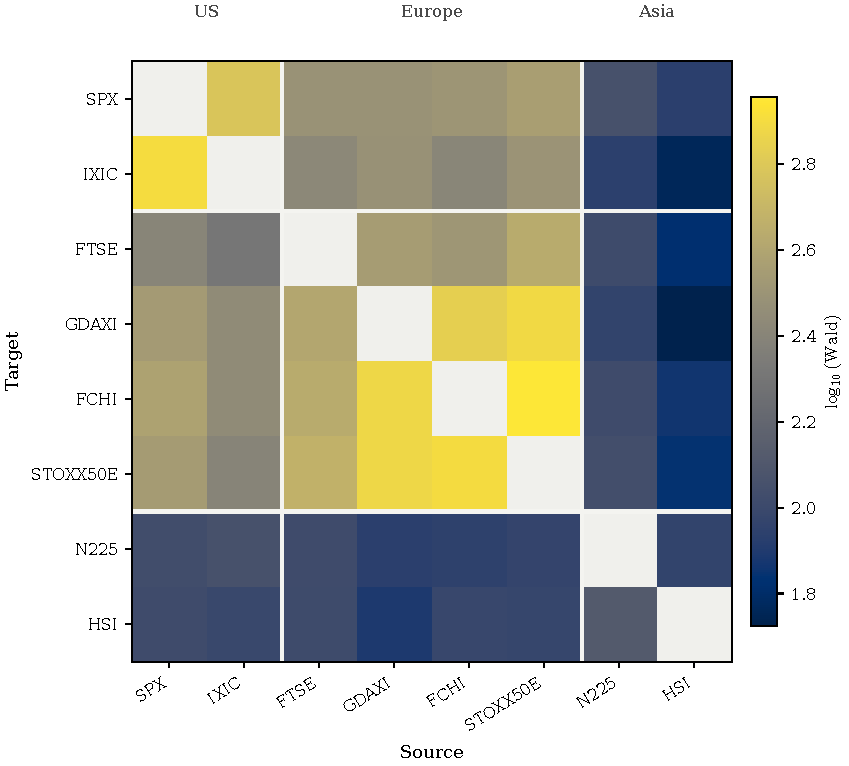
\includegraphics[width=0.94\textwidth]{figures/3-oxfordman-heatmap.pdf}
\caption{Directed source-screened intensity on the balanced Oxford-Man panel.  Darker cells denote
larger \(\log_{10}(\mathrm{Wald})\) values on the full 2000--2018 sample; the diagonal is
suppressed.}
\par\smallskip{\footnotesize\emph{Source.} Oxford-Man Institute realized-volatility library; authors'
projected-score calculations.\par}
\label{fig:oxfordman-heatmap}
\end{figure}

\subsection{Rolling observability and regime stability}

The rolling analysis uses 504-trading-day windows stepped every 21 trading days, which yields 171
windows for each pre-registered case-study pair.  The rolling results are reported as continuous Wald paths rather than rolling multiple-testing
labels.  Because the full-sample map is dense, the empirical object is the timing of strengthened or weakened
projected visibility, rather than first edge appearance.

Figure~\ref{fig:oxfordman-rolling} shows the four fixed case studies.  The two core transatlantic
links from SPX to STOXX50E and from STOXX50E to SPX both peak in the window from 2009-01-21 to
2011-04-13, with Wald statistics 125.5 and 134.6 respectively.  That build-up is gradual rather
than point-mass, but its crest falls in the neighborhood of the May 6, 2010 flash-crash episode.
The continental European pair from
GDAXI to FCHI peaks later, over 2012-02-22 to 2014-05-27, at Wald 172.2.  By contrast, the link
from SPX to HSI is much weaker, peaking only at 30.2 in the 2015-05-08 to 2017-08-04 window and
dropping below 1 in a near-null early-2000s window.  The rolling design therefore records
pronounced time variation even though the full-sample graph is uniformly visible.

\begin{figure}[htbp]
\centering
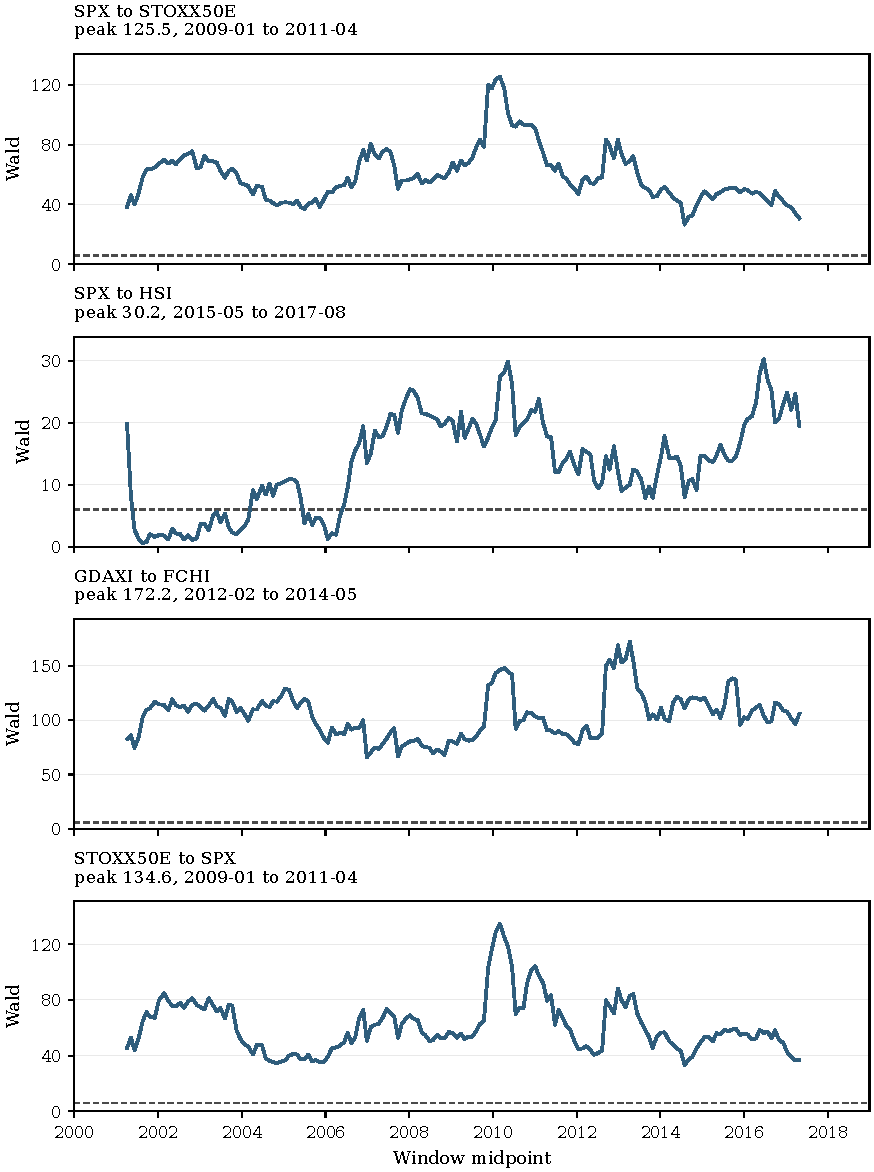
\includegraphics[width=0.92\textwidth]{figures/3-oxfordman-rolling.pdf}
\caption{Rolling source-screened Wald statistics for the four pre-registered case-study pairs.
Each panel reports one directed pair, and the dashed line marks the asymptotic \(5\%\)
chi-square threshold.}
\par\smallskip{\footnotesize\emph{Source.} Oxford-Man Institute realized-volatility library; authors'
projected-score calculations.\par}
\label{fig:oxfordman-rolling}
\end{figure}

\begin{table}[htbp]
\centering
\caption{Rolling summaries for the four pre-registered case-study pairs.}
\label{tab:oxfordman-rolling-summary}
\small
\begin{tabular}{lrrrl}
\toprule
Pair & full-sample Wald & median rolling & peak Wald & peak window \\
\midrule
SPX to STOXX50E & 348.8 & 56.5 & 125.5 & 2009-01 to 2011-04 \\
SPX to HSI & 103.4 & 13.9 & 30.2 & 2015-05 to 2017-08 \\
GDAXI to FCHI & 749.1 & 103.9 & 172.2 & 2012-02 to 2014-05 \\
STOXX50E to SPX & 364.8 & 56.5 & 134.6 & 2009-01 to 2011-04 \\
\bottomrule

\end{tabular}
\end{table}

\subsection{Scope of the P/Q interface in the Oxford-Man application}

The Oxford-Man application is a \(\PP\)-side market exercise.  It estimates realized roughness and
source-screened directed contagion under the physical measure, and it compares SPX only to an
externally cited projected option-surface roughness benchmark.  It does \emph{not} estimate a matched
option-panel covariance geometry and therefore does not produce pairwise pricing-visible,
path-detectable-only, or dynamically observable labels under both measures.  Those labels belong to
the matched-measure interface developed above, not to the realized-volatility panel used here.

The scope boundary matters.  Because the full-sample \(\PP\)-side network is dense,
realized-volatility data alone identify relative directed intensity and temporal stability.  A claim
that a pair is visible under \(\QQ\) but not under \(\PP\), or vice versa, requires a matched
option-panel implementation of the same projected geometry.  This section is a \(\PP\)-side
empirical benchmark.  It shows that the projected estimator is implementable on a balanced global
panel and that the SPX roughness discrepancy survives as a measured
\(\PP\)-versus-external-implied gap.


\section{Conclusion}

The threshold analysis separates pricing-visible smoothing contagion from contagion that is only
path-detectable \cite{vidal2026latent}.  The dynamic observability analysis identifies the
source-screened object that survives the reduction to observable filtrations
\cite{vidal2026dynamic}.  Here that object becomes an estimator.  The scalar
residual-product statistic remains the analytical benchmark, but the empirical estimator is the
projected covariance-score GMM statistic.

The governing object is the projected information matrix
\[
        \scrI_{\scrB}
        =
        \Gamma^\top\Omega^{-1}\Gamma .
\]
It determines local efficiency in the reduced Gaussian experiment, supplies the Wald noncentrality
constants, and measures how much source-screened information remains after the target-only tangent
has been removed.  Detection is therefore a statement about a covariance direction in a projected
LAN experiment, not about a raw spillover coefficient.

The asymptotic contribution has four parts.  The vector projected-GMM theorem gives the feasible
LAN and Wald limit.  The boundary-layer projected-rank theorem gives rough-regime identification
for \(H<1/2\).  The pilot roughness transfer theorem proves oracle equivalence under logarithmic
roughness accuracy.  The uniform minimax theorem upgrades the local Gaussian statement to uniform
rough-class optimality once the primitive reduction hypotheses are verified.

The estimator changes the empirical reading of contagion.  Weak rejection may be proximity to the
detection boundary rather than estimator failure.  Dense \(\PP\)-side panels should be summarized by
screened intensity and temporal stability rather than forced into sparse-edge language.  A
\(\PP/\QQ\) discrepancy is a mismatch between projected information geometries, not an informal
comparison of unrelated Hurst estimates.

The evidence stays inside those boundaries.  The synthetic experiments check the estimator at the
level of constants: null calibration, Wald-ratio calibration, and detection-boundary power.  The
Oxford-Man application shows that the same geometry is implementable on market data.  Physical
roughness remains stably rough, the SPX gap against the external implied benchmark is large, and the
global contagion map is dense but not temporally uniform.  Matched pairwise \(\PP/\QQ\)
classification requires option-panel data.  Its econometric object is already specified: a
projected information vector with separated labels for pricing-visible, path-detectable,
dynamically observable, target-confounded, and unidentified regimes.

The final claim is therefore bounded.  The paper gives a screened directional contagion estimand,
its projected local information geometry, and a feasible \(\PP\)-side estimator.  The matched-measure
interface maps the same estimator to risk-neutral pricing data, while the empirical application
remains faithful to the realized-volatility panel actually observed.

\appendix

\section{Supplementary calibration and data details}\label{app:supp-validation}

This appendix collects supplementary diagnostics and supporting tables.  They document the feasible
construction and robustness checks without interrupting the main text.

\subsection{Matched-cell feasible-pilot comparison}

The roughness pilot comparison is run on matched synthetic cells so that all pilot types are
evaluated on the same Monte Carlo draws.  Pilot improvements are overstated when different methods are compared on different random
realizations.  Table~\ref{tab:pilot-comparison} fixes the baseline empirical choice.  Adaptive
variogram-correlation is the default because it is stable across short and medium paths,
while the length-aware regime-adaptive extension serves as a targeted robustness enhancement for
longer upper-boundary cells where the correlation channel becomes more informative.

\begin{table}[htbp]
\centering
\caption{Matched-cell feasible-pilot comparison in the projected-score experiment.  Smaller is
better in every column.}
\label{tab:pilot-comparison}
\scriptsize
\begin{tabular}{lrrrr}
\toprule
Pilot & mean rel. info. & mean theta-gap & mean null Wald dist. & mean abs. log err. \\
\midrule
Variogram & 0.005885 & 0.041504 & 0.003780 & 0.133098 \\
Adaptive var.-corr. & 0.005593 & 0.038625 & 0.003878 & 0.124716 \\
Length-aware regime-ad. & 0.005529 & 0.038152 & 0.004270 & 0.122312 \\
\bottomrule
\end{tabular}
\end{table}

The trade-off is explicit.  The length-aware regime-adaptive construction is best on the
estimation-oriented metrics, but the simpler adaptive baseline is slightly tighter on null
Wald-ratio calibration.  The reported implementation therefore uses the adaptive pilot as the default
feasible implementation and treats the length-aware regime-adaptive pilot as a robustness rerun
rather than a replacement.

\subsection{Synthetic P/Q recovery design}

The P/Q mismatch functionals from Section~\ref{sec:scope-pq-rough} can be validated without market
data by constructing paired reduced experiments \((\PP,\QQ)\) with known covariance derivatives
\((A_P,A_Q)\).  The synthetic design is a controlled check that, when supplied with two
measure-specific covariance inputs, the projected estimator recovers the intended regime.  The paired synthetic design reports
\[
        \widehat\scrI_P^{\mathrm{src}\perp Y},
        \quad
        \widehat\scrI_Q^{\mathrm{src}\perp Y},
        \quad
        \widehat\scrI_P^{\scrB},
        \quad
        \widehat\scrI_Q^{\scrB},
        \quad
        \widehat D_I,
        \quad
        \widehat D_{\scrB},
        \quad
        H_{PQ},
        \quad
        \widehat c_{PQ}.
\]
The minimal regime grid is shown in Table~\ref{tab:pq-synthetic-grid}.  Each row is generated by
choosing synthetic derivatives with the displayed source-orthogonal information pattern and then
checking whether the mismatch functionals recover the correct label.  The formal target is
Theorem~\ref{thm:pq-label-consistency}: labels are expected to be stable only when the synthetic
population regime is separated from the classification boundaries.

\begin{table}[htbp]
\centering
\caption{Synthetic P/Q mismatch design.}
\label{tab:pq-synthetic-grid}
\small
\begin{tabular}{llll}
\toprule
Regime & Synthetic information pattern & Mismatch signature & Expected label\\
\midrule
P/Q equality & \(A_P^\perp=A_Q^\perp\neq0\) & \(D_I,D_{\scrB}\approx0,\ c_{PQ}\approx1\) & aligned\\
Pricing-visible & \(A_Q^\perp\neq0,\ A_P^\perp\approx0\) & \(D_I,D_{\scrB}\gg0\) & Q-only\\
Path-detectable & \(A_P^\perp\neq0,\ A_Q^\perp\approx0\) & \(D_I,D_{\scrB}\ll0\) & P-only\\
Dynamically observable & \(A_P^\perp,A_Q^\perp\neq0\), aligned & \(c_{PQ}\approx1\) & both\\
Direction mismatch & \(A_P^\perp,A_Q^\perp\neq0\), nonaligned & \(c_{PQ}\) small, \(H_{PQ}\) large & mismatch\\
Target-confounded & \(\|A_\mu\|>0,\ \|A_\mu^\perp\|\approx0\) & source information small & confounded\\
\bottomrule
\end{tabular}
\end{table}

\subsection{Oxford-Man panel coverage and robustness checks}

Table~\ref{tab:oxfordman-data-summary} records the balanced-panel coverage used in the main
application.  Table~\ref{tab:oxfordman-visibility-robustness} records the edge-count comparisons
underlying the statement that the full-sample \(\PP\)-side network is dense and
stable across the primary pilot and proxy reruns.

\begin{table}[htbp]
\centering
\caption{Balanced-panel coverage for the eight-index Oxford-Man application.}
\label{tab:oxfordman-data-summary}
\small
\begin{tabular}{llrr}
\toprule
Symbol & market & raw dates & balanced dates \\
\midrule
\texttt{.SPX} & S\&P 500 & 4620 & 4081 \\
\texttt{.IXIC} & Nasdaq Composite & 4616 & 4081 \\
\texttt{.FTSE} & FTSE 100 & 4639 & 4081 \\
\texttt{.GDAXI} & DAX & 4670 & 4081 \\
\texttt{.FCHI} & CAC 40 & 4691 & 4081 \\
\texttt{.STOXX50E} & Euro Stoxx 50 & 4691 & 4081 \\
\texttt{.N225} & Nikkei 225 & 4501 & 4081 \\
\texttt{.HSI} & Hang Seng & 4510 & 4081 \\
\bottomrule

\end{tabular}
\end{table}

\begin{table}[htbp]
\centering
\caption{Full-sample visibility checks on the Oxford-Man panel.}
\label{tab:oxfordman-visibility-robustness}
\small
\begin{tabular}{lccc}
\toprule
Run & visible pairs & baseline overlap & label changes \\
\midrule
Baseline (\texttt{rk\_parzen}, adaptive) & 56 & 56 & 0 \\
Pilot rerun (\texttt{rk\_parzen}, regime-adaptive) & 56 & 56 & 0 \\
Proxy rerun (\texttt{rv5\_ss}, adaptive) & 56 & 56 & -- \\
Proxy rerun (\texttt{bv}, adaptive) & 56 & 56 & -- \\
\bottomrule

\end{tabular}
\end{table}

\subsection{Supplementary calibration outputs}

The supplementary exercises report five procedure families on matched synthetic panels: the full
covariance oracle, the target-only covariance oracle, the source-orthogonal covariance oracle, the
scalar-anchor statistic, and the feasible projected-basis estimator.  Across these procedures the
reported diagnostics are organized around the same decision tree used throughout the analysis:
information decomposition, projected-rank and conditioning, null calibration, Wald-ratio
calibration, feasible-pilot stability, and, when supplied, paired synthetic P/Q interface
functionals.  Each experiment records:
\begin{enumerate}[label=(\roman*)]
\item information decomposition: \(\scrI^{\mathrm{full}}\), \(\scrI^{Y}\),
\(\scrI^{\mathrm{src}\perp Y}\), \(\scrI^{\scrB}\), \(\scrI^{\mathrm{scalar}}\), and capture ratios;
\item projected identification: \(\scrI_{\scrB,n}\), its eigenvalues, condition number, and
numerical rank;
\item calibration: null size under chi-square, multiplier, and empirical-null critical values,
reported separately for bandwidth zero and positive HAC bandwidths;
\item constant calibration: theoretical noncentrality, expected Wald mean, observed Wald mean, and
Wald ratio across a local-amplitude grid;
\item robustness extensions: theorem-matched Volterra blocks for \(H<1/2\), pilot roughness checks
reporting \(|\widehat H-H||\log h_n|\), \(\widehat\theta_n/\theta_n\), plug-in/oracle information
error, and Wald-ratio stability, non-Gaussian quasi-score panels with finite-difference loadings,
and paired synthetic P/Q interface recovery with separated-label checks.
\end{enumerate}
These diagnostics are the supporting record for the synthetic section; the appendix tables
above retain only the pieces needed to document pilot choice and empirical robustness checks.

\section{Primitive reduction proofs}\label{app:primitive-proof-modules}

This appendix records the auxiliary reduction results used in the article.  They are stated in
the notation of the projected covariance-score estimator so that the econometric argument remains
self-contained.

The first primitive lemma identifies the feasible realized-volatility proxy error at the block
level.

\begin{lemma}[Block log-realized-variance expansion]\label{lem:block-rv-expansion}
Let
\[
        \overline V_{k,n}^{a}
        =
        \frac1{h_n}\int_{I_{k,n}}V_s^a\,\dd s,
        \qquad
        a\in\{X,Y\}.
\]
Under Assumptions~\ref{ass:primitive-volterra}--\ref{ass:primitive-proxy-rate}, the block
log-variance proxy admits the decomposition
\[
        \widehat V_{k,n}^{a}
        =
        \overline V_{k,n}^{a}
        +
        e_{k,n}^{a},
\]
with
\[
        \frac1{N_n}\sum_k\EE[(e_{k,n}^{a})^2]
        =
        O(m_n^{-1})+O(h_n^{4H_a})+O(m_n^{-2}).
\]
Consequently the normalized target future and target past proxy errors are
\[
        O\bigl(h_n^{-H_Y}m_n^{-1/2}+h_n^{H_Y}\bigr)
        =
        o(1)
\]
in averaged \(L^2\), while the source past proxy errors are
\[
        O(m_n^{-1/2}+h_n^{2H_X})=o(1)
\]
coordinatewise, and remain negligible after summing over the \(J_n\)-dimensional memory window.
\end{lemma}

\begin{proof}
Conditional on the volatility path over \(I_{k,n}\), the return increments are centered Gaussians
with variances \(\Delta_n e^{2V^a}\), up to the discretization error.  The realized
variance is therefore a weighted chi-square perturbation of the integrated variance.  Taylor
expansion of the logarithm gives a martingale fluctuation of order \(m_n^{-1/2}\) and a quadratic
remainder of order \(m_n^{-1}\).  The replacement of integrated variance by
\(\exp(2\overline V_{k,n}^a)h_n\) costs \(O(h_n^{2H_a})\) in first order, hence
\(O(h_n^{4H_a})\) in squared error, by the \(L^2\)-H\"older regularity of the Volterra field.  The
target normalization multiplies adjacent block differences by \(h_n^{-H_Y}\); the source vector is
left on its unnormalized proxy scale.  The rate conditions in
Assumption~\ref{ass:primitive-proxy-rate} make the resulting averaged vector errors vanish.
\end{proof}

The covariance lemma identifies the frozen boundary-layer operator that enters every retained score.

\begin{lemma}[Boundary-layer covariance asymptotics]\label{lem:boundary-covariance}
For each local evaluation time \(t\), the latent Gaussian block covariance admits deterministic
frozen boundary-layer approximations
\[
        \mathbb G_t^{YY,(n)},\quad
        \mathbb G_t^{XX,(n)},\quad
        \mathbb G_t^{YX,(n)},\quad
        \mathfrak g_t^{Y,(n)},\quad
        \mathfrak g_t^{XY,(n)}
\]
such that, along the memory window \(J_nh_n\to0\),
\[
        \|\Sigma_n^{YY}-\mathbb G_t^{YY,(n)}\|_{\mathrm{op}}\to0,
        \qquad
        \|\Sigma_n^{XX}-\mathbb G_t^{XX,(n)}\|_{\mathrm{op}}\to0,
\]
\[
        \|h_n^{-H_{XY}}\Sigma_n^{YX}-\mathbb G_t^{YX,(n)}\|_{\mathrm{op}}\to0,
        \qquad
        \|h_n^{-H_{XY}}\gamma_n^X-\mathfrak g_t^{XY,(n)}\|_{\ell^2}\to0.
\]
The target-target and source-source blocks remain order one under their canonical normalizations,
whereas the source-target blocks enter at rough scale \(h_n^{H_{XY}}\).
\end{lemma}

\begin{proof}
Write each covariance entry as a double integral of Volterra kernels over two adjacent blocks.
Because \(j,\ell\le J_n\) and \(J_nh_n\to0\), all times used by the block vector lie in a shrinking
boundary layer near \(t\).  Replacing the smooth amplitudes \(L_i(u,v)\) by their diagonal values and rescaling
time by \(h_n\) gives deterministic frozen kernels on the discrete lag grid.  The singular powers
\((u-v)^{H_i-1/2}\) determine the normalizing factors.  The \(C^2\) amplitude remainder and the
discarded off-layer terms vanish in operator norm by Schur bounds on the resulting kernel matrices.
\end{proof}

The primitive rank proposition proves that the retained Volterra profiles have full projected rank
under nonsingularity of the profile Gram matrix.

\begin{proposition}[Primitive verification of boundary-layer projected rank]\label{prop:primitive-profile-rank}
Let \(\mathcal V\) be a compact rough Volterra class with \(H_{XY}\in[H_-,H_+]\subset(0,1/2)\).
Suppose Lemma~\ref{lem:boundary-covariance} holds uniformly over \(\mathcal V\), and let
\(\iota_n:\mathfrak H_\perp\to\R^{p_n\times p_n}_{\mathrm{sym}}\) denote the boundary-layer
discretization map from limiting covariance profiles to the whitened block covariance coordinates.
Assume \(\iota_n\) is asymptotically isometric on the finite-dimensional span of the derivative
profiles and that the feasible whitening and target-only projection are stable:
\[
        \sup_{\|c\|=1}
        \left\|
        \sum_{j=1}^m c_jA_{n,j}^\perp
        -
        \iota_n
        \left(
        \sum_{j=1}^m c_j\psi_j^\perp
        \right)
        \right\|_{\mathrm{score}}
        \to0
\]
uniformly over \(\mathcal V\).  For amplitude coordinates and Hurst coordinates the limiting
profiles are generated respectively by
\[
        u^{H_{XY}-1/2}
        \quad\text{and}\quad
        u^{H_{XY}-1/2}\log u,
\]
multiplied by the frozen diagonal Volterra amplitudes and then transformed by
\((I-\Pi_{\mathfrak Y})\mathcal W_t(\cdot)\mathcal W_t\).

If the source-screened profile Gram is uniformly nondegenerate,
\[
        \inf_{P\in\mathcal V}
        \lambda_{\min}
        \left(
        \bigl(
        \langle\psi_i^\perp,\psi_j^\perp\rangle_{\mathfrak H_\perp}
        \bigr)_{i,j}
        \right)
        \ge \lambda_*>0,
\]
and the retained dictionary approximates the derivative span uniformly,
\[
        \sup_{P\in\mathcal V}
        \sup_{\|c\|=1}
        \left\|
        (I-\Pi_{\scrB_n}^{\mathrm{score}})
        \sum_{j=1}^m c_jA_{n,j}^\perp
        \right\|_{\mathrm{score}}
        \to0,
\]
then the hypotheses of Theorem~\ref{thm:volterra-boundary-layer-rank} hold uniformly over
\(\mathcal V\), apart from the retained score covariance eigenvalue bound, which is supplied by the
projected-score CLT and HAC consistency result.
\end{proposition}

\begin{proof}
The uniform approximation display and the asymptotic isometry of \(\iota_n\) imply, uniformly over
\(P\in\mathcal V\) and \(\|c\|=1\),
\[
        \left|
        \left\|
        \sum_{j=1}^m c_jA_{n,j}^\perp
        \right\|_{\mathrm{score}}^2
        -
        \left\|
        \sum_{j=1}^m c_j\psi_j^\perp
        \right\|_{\mathfrak H_\perp}^2
        \right|
        \to0.
\]
This is the profile-convergence hypothesis in
Theorem~\ref{thm:volterra-boundary-layer-rank}.  The displayed Gram lower bound is exactly the
source-screened nondegeneracy hypothesis, and the dictionary display is exactly the span
approximation hypothesis.  Finally, differentiating the frozen rough kernel
\(u^{H_{XY}-1/2}\) with respect to \(H_{XY}\) gives the logarithmic profile
\(u^{H_{XY}-1/2}\log u\), while amplitude differentiation only changes the diagonal multiplier.
Thus amplitude and Hurst coordinates generate the profile family stated in the main theorem.
\end{proof}

The proxy-transfer proposition separates block-proxy error from covariance-score aggregation.

\begin{proposition}[Vector proxy replacement and projected-score transfer]\label{prop:vector-score-transfer}
Let \(Z_{k,n}^{\mathrm{lat}}\) be any centered Gaussian block vector, defined on the same
probability space as \(Z_{k,n}\), such that
\[
        \frac1{N_n}\sum_{k=1}^{N_n}
        \EE\bigl[\|Z_{k,n}-Z_{k,n}^{\mathrm{lat}}\|^2\bigr]\to0.
\]
Fix a projected covariance-score basis and write
\[
        d_{k,n}:=g_{k,n}-g_{k,n}^{\mathrm{lat}}.
\]
If the null covariance estimate, whitening map, target projection, and retained basis are stable in
operator norm, and if in addition
\[
        \frac1{\sqrt{N_n}}\sum_{k=1}^{N_n}\EE[d_{k,n}]\to0,
        \qquad
        \varepsilon_n^2
        :=
        \frac1{N_n}\sum_{k=1}^{N_n}\EE\bigl[\|d_{k,n}\|^2\bigr]\to0,
\]
and either
\begin{enumerate}[label=(\roman*)]
\item the proof is run on a disjoint block grid, so the score differences are independent across
blocks, or
\item there is a covariance envelope \(\widetilde\rho_n(\ell)\) such that
\[
        \sup_n\sum_{\ell\ge1}\widetilde\rho_n(\ell)<\infty
\]
and
\[
        \sup_k
        \left\|
        \Cov(d_{k,n},d_{k+\ell,n})
        \right\|
        \le
        \widetilde\rho_n(\ell)\,\varepsilon_n^2,
        \qquad \ell\ge1,
\]
\end{enumerate}
then
\[
        \frac1{\sqrt{N_n}}\sum_{k=1}^{N_n}
        \{g_{k,n}-g_{k,n}^{\mathrm{lat}}\}
        \toP 0.
\]
\end{proposition}

\begin{proof}
The deterministic component is the assumed aggregated mean remainder:
\[
        \frac1{\sqrt{N_n}}\sum_{k=1}^{N_n}\EE[d_{k,n}]
        \to0.
\]
This condition is needed at the \(\sqrt{N_n}\) scale; blockwise \(L^2\) convergence alone controls
variance, but it does not control an aligned deterministic bias.
If the proof is run on a disjoint grid, then
\[
        \Var\!\left(
        \frac1{\sqrt{N_n}}\sum_{k=1}^{N_n}
        \{d_{k,n}-\EE d_{k,n}\}
        \right)
        =
        \frac1{N_n}\sum_{k=1}^{N_n}\Var(d_{k,n})
        \le
        \varepsilon_n^2
        \to0.
\]
Under the covariance-envelope alternative,
\[
\begin{aligned}
        \Var\!\left(
        \frac1{\sqrt{N_n}}\sum_{k=1}^{N_n}
        \{d_{k,n}-\EE d_{k,n}\}
        \right)
        &\le
        \frac1{N_n}\sum_{k=1}^{N_n}\EE[\|d_{k,n}\|^2] \\
        &\quad+
        \frac{2}{N_n}
        \sum_{\ell=1}^{N_n-1}\sum_{k=1}^{N_n-\ell}
        \|\Cov(d_{k,n},d_{k+\ell,n})\| \\
        &\le
        \varepsilon_n^2
        \left(
        1+2\sum_{\ell\ge1}\widetilde\rho_n(\ell)
        \right)
        \to0 .
\end{aligned}
\]
Chebyshev's inequality therefore yields
\[
        \frac1{\sqrt{N_n}}\sum_{k=1}^{N_n}
        \{g_{k,n}-g_{k,n}^{\mathrm{lat}}\}\toP 0.
\]
\end{proof}

The HAC lemma characterizes the long-run covariance limit for the retained projected-score array.

\begin{lemma}[Projected-score HAC CLT and consistency]\label{lem:projected-hac-clt}
Let \(g_{k,n}\in\R^d\) be the retained projected score vector, with \(d\) fixed.  Suppose that,
after discarding \(O(1)\) boundary blocks, each row of the triangular array is stationary in the
block index \(k\), and that the centered array has uniformly bounded \(4+\varepsilon\) moments and
a dependence envelope \(\rho_n(\ell)\) satisfying
\[
        \sup_{k}\|\Cov(g_{k,n},g_{k+\ell,n})\|\le \rho_n(\ell),
        \qquad
        \sup_n\sum_{\ell\ge1}\rho_n(\ell)<\infty,
        \qquad
        \sum_{\ell>L}\sup_n\rho_n(\ell)\to0,
\]
with the usual triangular-array Lindeberg condition.  Then
\[
        \frac1{\sqrt{N_n}}\sum_{k=1}^{N_n}
        \{g_{k,n}-\EE g_{k,n}\}
        \toD N(0,\Omega),
\]
where the rowwise long-run covariance matrices
\[
        \Omega_n
        :=
        \Cov(g_{1,n},g_{1,n})
        +
        \sum_{\ell\ge1}
        \{\Cov(g_{1,n},g_{1+\ell,n})+\Cov(g_{1+\ell,n},g_{1,n})\}
\]
converge to \(\Omega\).  If \(L_n^{\mathrm{hac}}\to\infty\) and \(L_n^{\mathrm{hac}}/N_n\to0\),
the HAC estimator from Definition~\ref{def:vector-hac} is consistent for \(\Omega\).  In the iid
Gaussian calibration case, the bandwidth-zero estimator is the correct specialization.
\end{lemma}

\begin{proof}
Fix a vector \(a\in\R^d\).  The scalar array
\(a^\top\{g_{k,n}-\EE g_{k,n}\}\) has uniformly bounded \(4+\varepsilon\) moments, a summable
covariance envelope, and the stated Lindeberg condition.  The rowwise triangular-array CLT for
weakly dependent stationary rows gives
\[
        \frac1{\sqrt{N_n}}\sum_{k=1}^{N_n}
        a^\top\{g_{k,n}-\EE g_{k,n}\}
        \toD
        N(0,a^\top\Omega a).
\]
Cram\'er--Wold gives the vector CLT.  In the Gaussian quadratic-score case the required moment
bound follows from hypercontractivity of Gaussian chaoses of order two.

For HAC consistency, decompose the estimator error into the finite-lag sample covariance error, the
kernel truncation bias, and the long-lag covariance tail.  The finite-lag term vanishes because
\(L_n^{\mathrm{hac}}/N_n\to0\) and the rowwise moments are uniformly bounded.  The kernel bias
vanishes because \(K_{\mathrm{hac}}(\ell/(L_n^{\mathrm{hac}}+1))\to1\) for each fixed lag \(\ell\).
The tail term is controlled by
\(\sum_{\ell>L}\sup_n\rho_n(\ell)\to0\).  When the panel is iid, all lag covariances are zero
and bandwidth zero avoids estimating nonexistent dependence.
\end{proof}

\begin{remark}[Role of the scalar derivations]
The scalar residual-product derivations enter only through reusable ingredients: proxy reduction,
boundary-layer covariance, the target-only lower bound, scalar-anchor embedding, HAC normalization,
pre-averaging, and sieve stability.  The scalar residual-product testing theory is no longer the
main econometric object.  It is the benchmark submodel against which the projected covariance-score
GMM estimator is compared.
\end{remark}

\bibliographystyle{unsrt}
\bibliography{references}

\end{document}
